\documentclass{ucbthesis}
\usepackage[
    backend=biber,
    natbib=true,
    style=numeric-comp,
    sorting=none
]{biblatex}


% Disable indentation of subparagraphs
\makeatletter
\renewcommand\subparagraph{\@startsection{subparagraph}{5}{\z@}%
                                      {-3.25ex\@plus -1ex \@minus -.2ex}%
                                      {0.0001pt \@plus .2ex}%
                                      {\normalfont\normalsize\bfseries}}
\makeatother


% Undefine memoir version to prevent conflict with attrib
% https://tex.stackexchange.com/questions/297110/
\let\providelength\undefined
\let\providecounter\undefined


\usepackage{adjustbox}    % Auto-resize table content (eg Opo SenSys'14 rel)
\usepackage{pdflscape}       % Support landscape orientation for table
\usepackage{amsfonts}     % Adds math fonts, commands such as \begin{align}
\usepackage{amsmath}      % Provides align* environment
\usepackage{array}        % Tables for use in math mode
\usepackage{arydshln}     % Dashed lines in tables
\usepackage{attrib}       % Quote attribution formatting
\usepackage{balance}      % For balanced columns on the last page
\usepackage{booktabs}     % Elegant table-formatting library
\usepackage{bold-extra}   % Provides bf+sc (only in textbf+textsc env.)
\usepackage{bytefield}    % Formatting and layout of packets / bytefields
\usepackage{colortbl}     % Color table cells
\usepackage{comment}      % Provides \begin,\end{comment} for large blocks
\usepackage{cprotect}     % Allows verbatim, other formatting in macro args
\usepackage{enumitem}     % Additional control of enum/item environments
\usepackage{environ}      % Necessary for the placefigure creation
\usepackage{float}        % Allow use of [H] to force figure placement
%\usepackage{gensymb}      % Adds useful symbols w/out math mode, e.g. \degree
\usepackage{graphicx}     % For importing graphics
\usepackage{lipsum}       % For generating temporary filler text
\usepackage{listings}     % in-line source code (poorly, consider minted)
\usepackage{longtable}    % Tables that wrap across pages
\setlength{\LTpre}{0pt}   % No extra whitespace before/after
\setlength{\LTpost}{-25pt} % No extra whitespace before/after
\usepackage{mathtools}    % amsmath extension, adds more math formatting
\usepackage{mdframed}     % prettier boxes?
\usepackage[protrusion=true,expansion=true,kerning,spacing]{microtype} % better type, spacing
  \microtypecontext{spacing=nonfrench}
\usepackage{multirow}     % Multiple row spacing in tables
\usepackage{nth}          % Typeset 33rd correctly as \nth{33}
\usepackage{rotating}     % Rotates any object, note sideways != sidewaysfigure
\usepackage{makecell}     % Rotates any object, note sideways != sidewaysfigure
\renewcommand\theadfont{\normalsize}
% \DisemulatePackage{setspace} % allow to use with memoir
%\usepackage{setspace}     % Allow control of interline spacing with \setstretch
% https://tex.stackexchange.com/questions/15442/
\makeatletter
\let\@currsize\normalsize
\makeatother
%
\usepackage{siunitx}      % More units and things like \ohm
\usepackage{soul}         % Provides \hl{} for highlighting
\newcommand{\hlc}[2][yellow]{{\sethlcolor{#1}\hl{#2}}}
%
\let\subcaption\undefined
\let\subfloat\undefined
\usepackage[subrefformat=parens]{subcaption}   % Replaces both subfig and subfigure -- clashes with memoir from thesis cls?
\usepackage{tabularx}     % Complicated table creation
\usepackage{textcomp}     % Provides \textmu for upright mu's
\usepackage{threeparttable} % Add footnotes to a table
\usepackage{units}        % For nice fractions, \nicefrac{1}{2} --> 1/2
\usepackage{url}          % Pretty printing of hyperlinks
\usepackage[usenames,dvipsnames,svgnames]{xcolor} % Allow the use and definition of colors
\usepackage{xspace}       % Intelligently add spaces after commands
\usepackage{xfrac}
\usepackage[T1]{fontenc}

% The hyperref package must loaded last. Can conflict with some packages, see:
% README ( http://ctan.mackichan.com/macros/latex/contrib/hyperref/README.pdf )
\usepackage[colorlinks=true,linkcolor=black,citecolor=violet,urlcolor=Navy]{hyperref}     % Creates hyperlinks from ref/cite
\hypersetup{pdfstartview=FitH} % Sets default zoom to 100% width

% And, of course, cleveref must be loaded last-last (read: after hyperref)
\usepackage[capitalise,nameinlink,noabbrev]{cleveref}     % Do the right thing with fig/table references




% Break URLs properly (thanks to Alex Halderman)
\def\UrlBreaks{\do-\do\.\do\@\do\\\do\!\do\_\do\|\do\;\do\>\do\]\do\)\do\,\do\?\do\'\do+\do\=\do\#}
\def\UrlBigBreaks{\do\:\do\/}

% Don't typset URLs in tt font
\urlstyle{same}



% Set the graphics path
\graphicspath{{figs/}{images/}}



% Some macros that a broadly useful:
\newcommand{\uW}{{\textmu}W\xspace}
\newcommand{\uA}{{\textmu}A\xspace}
\newcommand{\um}{{\textmu}m\xspace}
\newcommand{\us}{{\textmu}s\xspace}
\newcommand{\uF}{{\textmu}F\xspace}
\newcommand{\uJ}{{\textmu}J\xspace}
\newcommand{\leeiic}{Lee~\iic}
\newcommand{\iic}{I$^2$C\xspace}
\newcommand{\vdd}{V$_{\textnormal{DD}}$\xspace}
\DeclareSIUnit\Wh{Wh}
\DeclareSIUnit\Ah{Ah}
\DeclareSIUnit\bit{b}
\DeclareSIUnit\byte{B}

% Some paper-specific things:
\newcommand{\name}{Permamote\xspace}
\newcommand{\namec}{Permacam\xspace}
\newcommand{\ssi}{\,\si}

% http://tex.stackexchange.com/questions/44330/side-brace-around-image-with-underbrace
\newcommand{\bracedincludegraphics}[2][]{%
  \sbox0{$\vcenter{\hbox{\includegraphics[#1]{#2}}}$}%
  \left\lbrace
    \vphantom{\copy0}
  \right.\kern-\nulldelimiterspace
  \underbrace{\vrule width0pt depth \dimexpr\dp0 + .3ex\relax\box0}}



\bytefieldsetup{endianness=big}

\newcommand{\colorbitbox}[3]{%
\rlap{\bitbox{#2}{\color{#1}\rule{\width}{\height}}}%
\bitbox{#2}{#3}}


% From bytefield package documentation:
%   facilitates the creation of memory maps. Start address at the bottom,
%   end address at the top.
%   syntax:
%   \memsection{end address}{start address}{height in lines}{text in box}
\newcommand{\memsection}[4]{%
  % define the height of the memsection
  \bytefieldsetup{bitheight=#3\baselineskip}%
  \bitbox[]{8}{%
    \texttt{#1}% print end address
    \\
    % do some spacing
    \vspace{#3\baselineskip}
    \vspace{-2\baselineskip}
    \vspace{-#3pt}
    \texttt{#2}% print start address
  }%
  \bitbox{24}{#4}% print box with caption
}
\newcommand{\memsectionhuge}[4]{%
  \bitbox[]{8}{\texttt{#1}}
  \wordbox[lrt]{1}{#4} \\
  \bitbox[]{8}{\dots}
  \skippedwords \\
  \bitbox[]{8}{\texttt{#2}}
  \wordbox[lrb]{1}{#4}
}


\definecolor{lightblue}{RGB}{0,204,255}
\definecolor{lightcyan}{rgb}{0.84,1,1}
\definecolor{lightercyan}{rgb}{0.95,1,1}
\definecolor{lightgreen}{rgb}{0.64,1,0.71}
\definecolor{lightergreen}{rgb}{0.84,1,0.87}
\definecolor{lightred}{rgb}{1,0.7,0.71}
\definecolor{OliveGreen}{cmyk}{0.64,0,0.95,0.40}
\definecolor{superlightgray}{RGB}{204,204,204}
\definecolor{lightgray}{RGB}{144,144,144}
\definecolor{light-gray}{gray}{0.75}
\definecolor{primary-blue}{HTML}{7D9FD3}
\definecolor{fig-green}{HTML}{2ca02c}
\definecolor{fig-purple}{HTML}{9467bd}
\newcommand{\glipsum}[1][1]{
  \textcolor{light-gray}{\lipsum[#1]}
}

% http://tex.stackexchange.com/questions/94892/how-to-use-short-subsection-title-in-header-but-not-in-table-of-contents
\newcommand{\markedsection}[2]{\section[#2]{#2%
\sectionmark{#1}}
\sectionmark{#1}}

\newcommand{\markedsubsection}[2]{\subsection[#2]{#2%
\subsectionmark{#1}}
\subsectionmark{#1}}



% https://texblog.org/2012/03/21/cross-referencing-list-items/
\makeatletter
\def\namedlabel#1#2{\begingroup
    #2%
    \def\@currentlabel{#2}.%
    \phantomsection\label{#1}\endgroup
}
\makeatother


% Pull in magic latex to separate figure placement from definition
\input{tools/placefigure}


\bibliography{references}

\begin{document}

% Declarations for Front Matter

\title{Yet to Be Named Thesis}
\author{Neal S Jackson}

% This text will appear on the title page
% This text will appear on the abstract page.
% For Berkeley, it should be identical to the graduation month.
\degreeyear{2022}
\degreesemester{Spring}

\degree{Doctor of Philosophy}

% COMMITTEE MEMBERS
% You can have up to 5 members listed separately.
% After that, you throw them all into the "other members" category.
\numberofmembers{3}
\chair{Associate Professor Prabal K.\ Dutta}
\othermembers{... \\
              ...}

% Previous degrees are no longer to be listed on the title page.
% \prevdegrees{B.A. (University of Northern South Dakota at Hoople) 1978 \\
%   M.S. (Ed's School of Quantum Mechanics and Muffler Repair) 1989}
\prevdegrees{} % Optional 


\field{Electrical Engineering}
% Designated Emphasis -- this is optional, and rare
% \emphasis{Colloidal Telemetry}
% This is optional, and rare
% \jointinstitution{University of Western Maryland}
% This is optional
\campus{Berkeley}


\maketitle
% Delete (or comment out) the \approvalpage line for the final version.
% \approvalpage
\copyrightpage

% ABSTRACT

%Battery-powered sensor nodes have long been the standard for simple and
%reliable sensor deployments, however they can suffer from short lifetimes and
%high maintenance costs associated with battery replacement.
%

For the past decade, the status-quo for energy harvesting sensors
has been to buffer small amounts of energy in capacitors to
intermittently work through a sensing task. While using capacitors for storage
offers these systems indefinite lifetime, it comes at a cost --
%While these systems avoid
%batteries, which are often dismissed as expensive, failure-prone, fragile, and
%temperature sensitive,
they must tolerate the decreased availability, lower energy utilization, and more complex programming models
inherent to a volatile, intermittent design.
We argue that many of these problems stem from insufficient energy storage and
could be eliminated with the use of batteries.  Recent advances in rechargeable battery
technology weaken the
historical arguments against their use. We believe that using batteries
in energy harvesting sensors will push us closer to a class of reliable,
general purpose devices that can better serve human-centric sensing applications
than their capacitor-based counterparts at the cost of having a finite, but long, lifetime.

%
%and new sensor designs that employ them
%will benefit greatly from the increased energy storage afforded by rechargeable
%batteries.
%
%While batteries do have a finite, but long, lifetime, their
%capacity allows future sensors to avoid
%costs and single-purpose designs associated with perpetual but
%intermittent sensors.
%poor availability, painful
%programming,

%This work bridges the gap between these two design points, advocating
%for the use of energy harvesting to extend the lifetime of
%a sensor node, exploiting rechargeable batteries to increase the
%utilization of harvestable energy, and relying on non-rechargeable batteries
%to ensure availability and avoid intermittency throughout the sensor's lifetime.
%We support this use of batteries by showing that many of the criticisms lodged against
%them are unfounded, outdated, or easily mitigated for the great majority of
%use cases. By modeling the charge-discharge patterns of
%energy stores in indoor harvesting
%environments, under both periodic and event-driven workloads, we show that this design
%can capture 1.5-2.2x the available energy of capacitor-only
%designs and achieve 4-6x the lifetime of primary-cell only designs, all
%while avoiding the poor availability, painful programming models, and special-purpose
%hardware platforms associated
%with intermittency.

%We support these claims by modeling the charge-discharge patterns of energy
%stores placed in real energy harvesting scenarios under periodic and event
%based workloads, and we defend our use of batteries by showing that
%the claims against them are either unfounded, outdated, or easily mitigated
%for the vast majority of real use-cases.
%
%
%
%By modeling the charge-discharge patterns of energy stores placed in real
%energy-harvesting scenarios under periodic and event-based workloads, we show
%the performance increases associated
%
%of
%the sensor node. To support these decisions we model the charge-discharge patterns
%of energy stores when placed in real, energy-harvesting scenarios under periodic
%and event-based workloads,
%
%
%
%By forgoing the high capacity of
%batteries however, these everyla
%
%
%however they inherently trade-off
%availability
%
%Harvesting ambient energy to power distributed sensor nodes has the
%potential to extend their lifetimes and increase their performance compared
%to non-harvesting, battery-powered designs. Sensor platforms presented
%in prior work take advantage of this harvested energy by temporarily storing it in
%capacitors before using it to perform a small number of operations, intermittently
%working through a sensing task. Some authors
%
%Energy harvesting has the potential to extend the lifetime and increase
%the available
%
%however current
%energy harvesting architectures
%
%Energy harvesting has the potential to power distributed sensing nodes,
%extending their lifetimes, increasing the energy available to
%perform sensing tasks, and reducing the maintenance cost of a sensor
%deployment. In the past five years a trend has even
%emerged pushing for ``perpetual'' batteryless sensors,
%supported by claims that batteries are fragile, toxic, temperature
%sensitive, and prone to long-term cycling failure. Alternative
%designs temporarily store harvested energy in capacitors before performing
%a small number of operations, intermittently working through a sensing task.
%These intermittent designs, however, are inherently prone to low availability
%for many workloads, present users with non-standard programming models to mask
%their intermittency, and make poor utilization of the harvestable ambient
%energy.
%
%We argue that utilizing batteries, both rechargeable and non-rechargeable cells,
%can solve these problems for the vast majority
%of real workloads and deployment scenarios while still providing
%the key benefits of energy harvesting.
%By analyzing the availability, lifetime and harvestable energy utilization
%for a variety of energy storage systems we motivate the need to use
%batteries, and we welcome their use by
%showing that many claims against them are unfounded, outdated or easily mitigated.
%To perform the analysis, we model the charge-discharge patterns of
%energy stores when placed in real, energy-harvesting
%scenarios under periodic and event-based workloads, and we evaluate this
%model by comparing it to implementations of several points in the design space.
%We show that for reasonable energy storage sizes, workloads, and
%energy availability, sensor
%nodes utilizing batteries along with energy harvesting can capture \hl{6x} the available
%energy of capacitor-only designs and achieve at least \hl{4x} the lifetime of
%primary-cell only designs, all while avoiding the poor availability and painful
%programming models associated with intermittency.


\begin{frontmatter}

\begin{dedication}
\null\vfil
\begin{center}
...
\end{center}
\vfil\null
\end{dedication}

% You can delete the \clearpage lines if you don't want these to start on
% separate pages.

\tableofcontents
\clearpage
\listoffigures
\clearpage
\listoftables

\begin{acknowledgements}


\end{acknowledgements}

\end{frontmatter}

\pagestyle{headings}

% (Optional) \part{First Part}

\begin{definefigure}{fig:platform}
\includegraphics[width=\columnwidth]{images/platform_quarter.jpg}
\vspace{-2\baselineskip}
\caption{ \name{}. 
    \normalfont{A wireless camera platform for indoor computer vision applications. To achieve a multi-year lifetime, we employ energy harvesting with a photo-voltaic panel. A quarter is included for scale. \name is capable of local inference as well as full image transmission to cloud image processing pipelines. The platform is 10\,mm thick, and has a rechargeable and non-rechargeable battery on its backside}
}
\end{definefigure}
\placefigure{fig:platform}

\section{Introduction}
Image inference, including classification and object detection, has been one of the most active areas of computer science and machine learning research. However, due to the cost and difficulty of deploying wired cameras, applications based on continuous image sensing is untenable. This is especially true for indoor applications, where camera density must be higher for sufficient coverage.

Indoor wireless camera sensors have been heavily researched and commercialized over the past fifteen years, but due to the technology available at the time, as well as incompatibilities between design decisions and longevity, these platforms are typically limited to lifetimes of at most weeks to months~\cite{rowe2007firefly,rahimi2005cyclops,blinkindoor,wyzeoutdoor,josephson2019wireless}. 
Deployment of these platforms beyond small or temporary installations remain a challenge due to the cost of frequent battery replacement.
With the confluence of new and improved COTS technology, like low power processors, radios, and image sensors, it is worth revisiting the design of wireless camera sensors. 

Recent improvements in microcontrollers go beyond lower power \cite{kim2018system}. Processors now include hardware floating point support, single cycle multiplies, and data-parallel instruction (SIMD) support. The promise of new dedicated accelerators provides the potential of significant improvements in inference performance on low power systems~\cite{armm55,himaxwiseeye}. This has led to renewed interest in performing complex local inference on a battery budget, especially as transmitting large data like images is traditionally very expensive. However, radios have also become far more power efficient, which again muddies the conventional wisdom. Indeed, it is now much cheaper to transmit large data to a more capable system. Desktop or server class machines handily outclass their low power microcontroller and accelerator brethren on performance, providing the ability to perform more complex and accurate inference, if only data can be efficiently delivered to them.
%Regardless of recent improvements, microcontroller and accelerator performance will continue to pale in comparison to desktop and server class computing systems. 
This is especially true as memory has not scaled at the same pace as processing.
This rapidly changing design space points to a requirement for a flexible architecture and framework for thinking about what applications are most suited for local processing versus cloud offload.
% or data transmission.

In this work, we present \name, the first wireless, energy-harvesting camera platform capable of capturing and transmitting an image every ten minutes for half a decade in indoor environments.
\name represents a culmination of recent work on low power camera sensors~\cite{josephson2019wireless,nardello2019camaroptera,naderiparizi2015wispcam} and energy harvesting sensor platforms~\cite{jackson2019capacity}. \name features a hierarchical energy harvesting system that couples a small rechargeable battery with a backup non-rechargeable battery. This combination provides the system with a long and reliable lifetime. The longevity and reliability of the platform make it suitable for long-term, low-maintenance deployments. Images captured by \name are capable of driving applications based on object detection, like people counting or interaction tracking. With default, pretrained weights, an object detection model is able to detect a person in \name images from 20 meters away.

\name is capable of performing both local inference and transmitting full images end-to-end to more powerful systems. Local inference potentially requires less energy than image transmission, and also provides significantly better privacy guarantees. In cases where privacy is not as much of a concern, image transmission to a more capable endpoint increases the flexibility and performance of inference run on images. Privacy can still be guaranteed if images are transmitted only within a local network.
We examine the implications of both architectural choices with respect to capability, energy, and latency.

Our results show that on modern SoCs, transmitting images surprisingly enables longer lifetimes and improved inference. While this conclusion is unique to indoor wireless camera sensors 
whose footprints are not dominated by their energy harvester or storage, its general methodology can be applied to other application spaces as well.
%
Through this conclusion, we develop an end-to-end architecture that makes images captured by \name accessible to data collectors and application builders. \name provides a scalable and easily deployable method to quickly gather visual data for machine learning training or datasets. Images collected by \name are easily integrated into popular computer vision and machine learning frameworks like OpenCV, TensorFlow, and PyTorch. Using these tools, high level applications can be built to drive visual applications like building occupancy counting for more efficient energy management and critical infrastructure monitoring atop a long-lived deployment of wireless \name devices.

%Additionally, privacy is a serious concern, and we demonstrate that \name is capable of some local inference. In cases where applications require capability over privacy, images can be transmitted end-to-end to the cloud, or to a more local endpoint. 
%This provides the option to still maintain some privacy when transmitting images.




\chapter{Wireless Sensor Network Applications and Power Supply Design}

\hl{rework this}\\
The popularity of batteryless designs in the research community has increased over the past decade. This popularity has resulted in a focus on improving the design of these systems to mitigate their drawbacks. 
The end goal of batteryless researchers is to create a design pattern that can be reused for general-purpose applications, resulting in a fixation on design, without sufficient grounding in real applications~\cite{hester2017future}. The reality is that the batteryless archetype will never be able to provide a general purpose solution for reliable and consistent sensing, and is only appropriate for niche applications.
This chapter explores the landscape of wireless sensor power supply design and applications,
identifying several overarching design archetypes and
grounding the design process through an application-focused lens.
By abandoning previous assumptions 
%about the necessity of the batteryless archetype, 
and starting with a blank slate and a wholistic view of available technology and application requirements, we can return to application-focused power supply design to create simpler, long-lived, and reliable solutions.
%This chapter defines common wireless sensor power supply design archetypes, and situates these archetypes within a deconstructed view of the application landscape. 

\section{Application Space}

The design of a wireless sensor power supply should follow the requirements of an intended application.
Application requirements define the parameters of the various components of a wireless sensor power supply, such as the size, lifetime, or efficiency of a harvester and energy storage.
Given an application, a set of questions should be asked to define its requirements and better define design parameters.
While not an exhaustive list, an appropriate set of questions to help define the power supply requirements could resemble the following:

\begin{enumerate}
    \item What area and volume is available for energy harvesting and energy storage?
    \item What are the average power requirements for the application?
    \item How much harvestable power is available?
    \item What is the maximum atomic energy quanta required by the application?
    \item What is the application lifetime requirement?
    \item Does the application require reliable operation?
\end{enumerate}

In the following subsections, these questions are explained and more deeply explored. In \cref{chap:intuition}, these questions form the basis of formalizing a set of high-level constraint equations to describe power supply design.

\subsection{Size}

\subsection{Power}

\subsection{Harvesting Potential}

\subsection{Atomicity}

\subsection{Lifetime}

\subsection{Reliability}





\section{Power Supply Design Archetypes}

All wireless sensors require electrical energy to function. 
That energy must either be allocated prior to deployment, or provided or collected during deployment. 
The archetypes presented in \cref{fig:background:archetypes} represent the high-level architectural possibilities for storing energy and powering wireless sensors.
Energy storage and harvesting technology is rapidly improving, and varied application requirements will result in different design parameters. Despite this, the power supplies for all wireless sensors can be divided into clearly delineated design patterns. 
Most simply, energy can be provisioned in a finite energy storage like a battery, also known as a primary cell. In situations where there is harvestable energy, it can be captured and stored in rechargeable storage, or a secondary cell. 
If the available harvestable energy is on or below the edge of being sufficient to fully power a sensor and its workload, harvesting can be paired with a backup primary source to ensure consistent, reliable operation with an extended lifetime. 
These three classes of design archetypes encompass the options for wireless sensor power supplies, if not for all electronic devices. 
The next few sections explore the gradient of design space in more detail, and identify existing systems and their place within the design space. 

\subsection{Primary-only}
Non-rechargeable (primary-cell) batteries have been the preferred
method of powering sensors for both academic experimentation
and commercial and industrial applications. 
The Telos family of motes, originally designed in 2004~\cite{polastre2005telos},
is still the wireless platform of choice for some modern research projects~\cite{mohammad2018codecast,li2019privacy}.
The Hamilton mote is an example of an attempt to provide a more modern, cost-effective alternative to older motes~\cite{andersen2017hamilton}.
Besides research platforms, the majority of commercial smart home sensors, like those offered by Ecobee, Honeywell, Lutron, Nest, Phillips, among many others, all opt to use non-rechargeable batteries as their source of energy~\cite{ecobeeSensor, honeywellThermostat, lutronSolutions, googleNestTemperature, hueSensor}. Industrial offerings from Emerson, GE, Honeywell, and others also utilize non-rechargeable power cells in their reliable wireless sensors~\cite{emersonRosemount,GEInsightMesh,honeywellOneWireless}.
The use of primary-cells is popular in commercial and industrial sensing because they enable sensors with predictable lifetimes that are easy to
design, simple to program, and reliable to operate. 
A finite energy storage provides a finite lifetime, meaning battery replacement is inevitable. However, advances in energy efficiency and battery technology have resulted in reliable sensors that can last up to 10 years without battery maintenance~\cite{emersonRosemount,honeywellOneWireless, lutronSolutions}. 

\subsection{Energy Capture with Buffer}
%Prior work regarding energy-harvesting sensor systems can be broadly
%divided into two categories: those which make use of intermittent computing
%techniques and those which do not.
%Intermittent systems often exist in a regime of unreliable and ultra low harvester power, where
%operation and uptime are not guaranteed. As such, they often lose power and
%reboot while intermittently working through a sensing task.
%A wealth of work has been devoted to
%making these systems usable and reliable.
%Other energy-harvesting systems, especially those deployed outside, have access
%to significantly more harvestable energy and are able to store more of this energy
%for later use, so they
%do not use intermittent computing techniques to complete their workloads.

Instead of preallocating energy, a system can utilize external sources of energy.
The quantity, and consistency of external energy can vary widely. If the energy is predictable or reliable, a system can be powered entirely from the external source. If the source is unpredictable, captured energy can be stored or buffered in rechargeable storage, generally a (super)capacitor or battery to use in times where external energy is unavailable. 

At one extreme of power delivery, a wireless sensor can be powered by a reliable source, like wired power.
As much as it seems like an antithesis to "wireless" sensors, wired power is a solution for a class of applications where using a battery is more costly than installing wired power. 
This is especially true for applications that are monitoring powered devices or measuring mains power. 
For example, the Powerblade power meter is connected to AC mains power for both measurement and power supply~\cite{debruin15powerblade}. 
Its proximity to readily available AC power and its small form factor make the inclusion of a battery infeasible compared to scavenging off mains power.

The majority of wireless sensors that depend on external sources of energy are energy-harvesting. They utilize 
%e, energy harvesting that is utilized in environments with sparse and inconsistent energy results in extremely low power designs, and designs that operate intermittently. 
photovoltaic, thermoelectric, piezoelectric, ambient RF harvesting or other methods to scavenge energy from their environment.
This results in limited and unreliable energy income.
Parameters like harvester size or surface area, and harvesting method, impact the amount of potential power delivered to the sensor, while the size and capacity of the rechargeable storage determines how much energy can be buffered.
This device class can be further differentiated by how captured energy is stored. Intermittent, or batteryless systems, eschew both non-rechargeable and rechargeable batteries and utilize capacitors and supercapacitors for energy buffering. The choice of a (super)capacitor buffer significantly limits the amount of energy capacity available to the system, reducing its capability to cache energy in times of drought. This choice is predicated on the assumption that rechargeable batteries are less suitable for energy harvesting applications. However, most energy harvesting systems, particularly those that utilize outdoor photovoltaic harvesting, utilize rechargeable batteries.

\subsubsection{Batteryless}
\label{sec:related:batteryless}

Energy-harvesting systems that rely
on small (super)capacitor energy buffers are commonly referred to as intermittent systems, as they only store enough energy to perform single atomic tasks, and are unable to operate when external energy is not present.
Many choose to employ
capacitors as an energy buffer due to their theoretically infinite lifetime,
but are limited to small energy capacities, and are only as reliable and
lively as their source of harvested energy.
In situations of energy drought, 
these platforms quickly deplete their 
small energy stores, and lacking energy,
they power off and lose
state, potentially in the middle of an important operation or for an extended period of time.
Due to this reality, researchers have spent the past decade
designing more predictable and usable batteryless systems. This has resulted in several different hardware and software design methods and techniques for intermittent systems.
\\

\noindent
\textbf{One-shot Intermittency.}
One of the simplest methods employed by batteryless systems ignores the difficulty associated with completing longer workloads, and instead just allocates enough capacitance to turn on and perform a simple task, like sending a radio packet. This method is reminiscent of the simple reply behavior of RFID tags, upon which the design of early intermittent systems is based on~\cite{sample2008design}. These systems may act as a simple beacon~\cite{campbell2016cinamin,saoda2019no}, or act as an actual sensor~\cite{debruin2013monjolo, campbellEnergy14, campbellThermes14}.
%The Gecko and Monjolo platforms ignore the difficulties associated with
%completing longer workloads and instead allocate
%just enough capacitance to turn on and perform a simple task. 
For some platforms, most notably the Monjolo family of devices, the rate of harvesting is used as the sensor itself. Every wakeup and transmit event corresponds to an amount of energy harvested, and can be used to quantify the harvested phenomenon~\cite{campbellThermes14, campbellEnergy14, debruin2013monjolo}.
However, this approach can require application specific
and tedious optimization of the cold start process and is severely
limited in its generality. Performing any sensing or computing outside of the
hardware's intended use case is often not possible.
Like all intermittent sensors, it is also difficult to distinguish between sensor failure and a lack of energy.
\\

\noindent
\textbf{Checkpointing.}
To address the limited generality afforded by capacitor energy storage, researchers have developed software frameworks, programming language primitives, and debugging tools that allow forward progress on energy intensive tasks. 
%Other work in this space attempts to cope with
%intermittency
%by 
%developing tools and
%programming language primitives that allow %can perform
%complex and energy intensive tasks to execute despite limited energy storage.
Intermittent-aware programming
models and compilers enable checkpointing and progress latching over
workloads that may require more energy than can be stored
~\cite{lucia2015simpler, ransford2012mementos, hesterTimely17}. 
New debugging tools
spanning both the hardware and software domains
measure the energy required for specific code operations
and restore energy state during code breakpoints~\cite{colin2016energy}.
\\

\noindent
\textbf{Hardware Hysteresis Management.}
In addition to intermittent software techniques, researchers have developed
hardware platforms to
increase availability and responsiveness through the fine-grained management
of capacitor charging hysteresis.
For these systems,
it is often assumed that the upper hysteresis threshold, the point at which a
charging device turns on, is the voltage at which a capacitor is full, and the
lower threshold, the point at which the system turns off or sleeps, is the minimum
operating voltage of components in a system.
Smaller capacitors can charge to an upper
threshold and turn on faster, but store less energy.  Hysteresis management
techniques attempt to combine different sized capacitors to
minimize charging time while also maximizing available energy.

Notable examples of this technique are the Flicker and Capybara platforms~\cite{hesterFlicker17, colinReconfigurable18}.
The Flicker
platform employs federated
energy storage in which each peripheral has its own storage tuned to the task
it is expected to perform~\cite{hesterTragedy15,hesterFlicker17}. This has the
effect of allowing various components to charge their storage quickly and turn on before other parts of the system, as well
as isolating power failure to independent components.  
The Capybara platform also manages capacitance,  
but provides even more flexibility by dynamically resizing its banked
capacitor store to match the energy required by a task
~\cite{colinReconfigurable18}. This leads to the lowest possible cold start and capacitor recharge times to support a given operation.

The assumption that device operation should be coupled to full-swing hysteresis is a questionable one. 
While the design decisions to manage capacitance make sense in the intermittent context, the importance placed on cold start optimization is specific to the power efficiency of a design, and limited energy capacity. 
Capybara's power supply has a significant
"power overhead of the power system" that limits the effectiveness of
sleeping~\cite{colinReconfigurable18}. The energy storage provided by capacitors and small supercapacitors is also very limited, making it difficult to sustain a sleeping state for a long time. 
Due to this, most intermittent system designs opt to fully discharge energy storage on every operation instead of sleeping and instead focus on optimizing cold start.  
In practice, if a system has the ability to enter a low power sleep mode with state retention, it can avoid frequent cold start and control its energy usage by willfully entering these
states. 
Cold start is expensive, as harvesting ICs and boost converters are optimized for steady state operation and not cold start efficiency. This results in wasted energy and time on charging a capacitor to a working voltage.
%With this operating principle, the benefits of hardware hysteresis management are limited to reducing cold start time and are workload independent.

These complex software and hardware solutions, while increasing usability and reactiveness of batteryless systems, has not led to widespread adoption by industry. 
While a few companies are developing batteryless products, including EnOcean, Perpetua, and Everactive~\cite{enocean, perpetua, everactive}, the majority still employ non-rechargeable batteries.
This is because existing intermittent work has not been able to address the singular problem for (super)capacitor-based energy
harvesting systems: in the face of plentiful harvestable energy, they are not
able to store the energy for later use (in times of energy drought).
As a result, they must
micro-optimize the little energy they have. 
In many applications, if these
systems had sufficient capacity, they could capture a greater share of available energy, and simply adjust sensing rate and
sleep periods to achieve energy-neutral operation. 
%We show that the energy captured
%by these systems and their subsequent availability
%could be substantially improved by using larger energy buffers.

\subsubsection{Non-intermittent Sensors}
\label{sec:related:nonintermittent}
Non-intermittent energy-harvesting sensors
have largely existed in environments with plentiful harvestable energy
and have been designed with sufficient capacity to capture this energy. 
%Some
%devices have also embraced backup primary-cells to further ensure
%reliable operation.  
%In the middle, in environments with sufficient and predictable available energy, designs can scavenge energy and store it in a rechargeable battery to power their workload. 
Most examples of such devices are deployed outdoors with photovoltaics~\cite{jiang2005perpetual, kansal2007power, corke2007long, lin2005heliomote, adkins2018signpost}. 
%Energy harvesting in industrial environments is also possible with sufficient heat differential or vibrational sources~\cite{perpetua, kinergizer}. 
%However, the adoption and application of such harvesting methods is limited and non-rechargeable batteries remain the most popular option for powering industrial sensors.
%Notably, Prometheus utilizes a supercapacitor as a short term energy store, and when full,
%charges a backup rechargeable lithium battery~\cite{jiang2005perpetual}. At
%the time of its design, lithium cells offered highly limited recharge cycles,
%and by utilizing a supercapacitor, much of this
%charge-discharge volatility was masked from the secondary-cell, extending its lifetime.
Non-intermittent sensors have also been employed indoors. 
The EnHANTs sensor uses an indoor photovoltaic panel to charge an intentionally oversized NiMH
battery, with plans to eventually use a thin-film battery~\cite{margolies2015energy}.
DoubleDip utilizes thermoelectric harvesting to charge a lithium-manganese battery~\cite{martin2012doubledip}
These examples are of older designs, using older battery technology that had limited cycle lifetimes. However, the greater energy capacity provided by batteries allows these designs to avoid the complications of intermittency and batteryless operation.
The popularity of batteryless systems has led to a distinct lack of modern research systems that utilize rechargeable batteries, especially those that are not outdoors.

%DoubleDip notes that supercapacitors offer
%lower energy density and higher leakage when compared to batteries, but admits
%that the lithium-manganese chemistry suffers from low maximum output currents
%and a limited number of charge-discharge cycles.
%While the limitations of past batteries have slowed their adoption in
%low energy-harvesting scenarios, we claim that recent developments in battery
%technology will enable higher capacity energy storage without these trade offs.


\subsection{Energy Capture with Buffer and Primary}

Regardless of which energy store is used, energy-harvesting systems will
experience some degree of uncertainty regarding energy income. 
A non-rechargeable
backup energy store can be utilized to mask this uncertainty, cold
start electrical components, and provide consistent, reliable, and lively operation.
A third design archetype is a combination of the first two: 
external energy capture paired with a backup non-rechargeable cell.
While this archetype makes sense from the perspective of maximizing system lifetime and reliability, it is not commonly employed. 
The Pressac line of supercapacitor-based energy-harvesting sensors 
use a battery backup to obtain an estimated 10 years of continuous, reliable operation~\cite{pressac}.  
%This work suggests that these sensors could significantly
%increase their lifetime by using a larger secondary energy store.
There has been little
exploration on the benefits of this hybrid design and the use of
primary-cells to avoid intermittency,
and provide baseline reliability. This dissertation seeks to explore this design point in more detail.





\chapter{
Heuristics for System-Level Power Supply Design 
}
%system level

%Intuition for Wireless Sensor Power Supply Design
%Navigating design space
%Guidelines
%Entanglements
% more active titles
\label{chap:intuition}

%There is a rift between industry and research in the way that indoor wireless sensors are powered. Industry has largely eschewed energy harvesting methods, opting instead for the reliability offered by high-density non-rechargeable batteries. 
%Conversely, energy-harvesting is extremely popular for research systems, which have largely abandoned the use of non-rechargeable cells in the pursuit of building systems with indefinite lifetimes. 
%Given this disparity, it is obvious that there is a lack of clarity regarding how wireless sensors should be powered to enable various applications. 
Wireless power supplies are the result of a multi-dimensional design space exploration.
While certain design decisions are straightforward, like the choice to use a certain type of harvester to suit an application environment, some design points are more difficult to determine. 
Harvesting and storage technologies are often difficult to directly compare, and it is sometimes difficult to determine the sizing of these elements in order to satisfy the constraints of an application. 
Many times, the type and size of harvesters, batteries, or capacitors are chosen arbitrarily~\cite{hamiltoniot,lee2013modular,juang2002energy}, or are chosen to make the design minimally feasible~\cite{yervaGrafting12,debruin2013monjolo,hesterFlicker17,afanasov2020battery}.

The goal of this chapter is to provide high-level guidance for navigating the design space of wireless sensor power supplies. 
We formalize the the application requirements that were discussed in 
\cref{sec:background:background_reqs}.
Using these requirements, this chapter provides guidance to designers for when energy harvesting is a beneficial technique for energy income instead of, or in addition to, a non-rechargeable storage, how prospective income and workloads drive component types and sizing, and if energy-harvesting is utilized, what techniques are required to ensure a minimum useful operation or what is required to capture sufficient energy to maximize system availability. 
To limit scope of this chapter among those following to a manageable size we choose to focus exclusively on indoor photovoltaic energy harvesting.
%This is because in the conditions of the majority of human-occupied indoor locations, photovoltaic harvesting offers an order of magnitude more energy than other methods.
%Despite this focus, similar explorations can be made with other harvesting methods.
Occupied indoor environments are the focus of a significant
amount of
prior work, 
and for good reason: most
applications aim to improve the lives of people and are necessarily present
in the spaces they occupy~\cite{hesterTimely17,hesterFlicker17,colinReconfigurable18,campbellEnergy14} \hl{TODO better cites}.
%Even the example applications of intermittent, energy harvesting systems are nearly all centered around monitoring
%indoor and human-centric phenomena
Indoor environments are lit by both natural and artificial light, 
and may occasionally get direct or indirect sunlight. 
Under these conditions, photovoltaic harvesting still offers an order of magnitude more energy than other methods.
However, indoor environments still present a significantly more challenging and low power design space compared to the outdoor ones. 
The decision to focus on indoor photovoltaic harvesting does not mean that the conclusions drawn are not applicable to other
environments and harvesting methods, however design details may differ. 

\section{Energy Income}
\label{sec:intuition:energy_income}
A wireless sensor must source energy from somewhere. 
Energy-harvesting has the potential to supply energy indefinitely. However, harvested energy is often unreliable and unpredictable, and instantaneous power delivery is limited. 
Conversely, primary-only systems have a limited amount of energy, but can use that energy at any rate they please, within the power limits of the battery. 
Because of these differences, it can be difficult to directly compare their performance and determine at what scale and in which conditions harvesting, energy preallocation, or a hybrid of the two, is the preferable power source strategy for any given application.
This section begins with a description of constraints for properly sizing components to ensure a sufficient lifetime and energy income. 
Next, it provides a method of comparison of energy capture potential between harvesting and preallocation methods.
The constraints and relations defined and explored in the following section can be used to estimate proper harvester and battery selection to achieve application requirements.

\subsection{Sizing}
\label{sec:intuition:energy_income_sizing}
Regardless of how a sensor is powered, it must receive sufficient energy at the right times to continuously and reliably operate.
Assuming that the average power required to drive an application is known at design time, it is relatively straightforward to determine the correct size of a battery to achieve an expected lifetime, or a photovoltaic panel to achieve an average power income.
%The improvement in energy density of batteries and the efficiency of energy harvesting sources has not improved at the same rate as the energy efficiency of CMOS and low power radio technology.
%Barring any transformative improvements in energy storage, energy income is primarily dependent on the volume or area available for a battery or harvester, respectively. 
Usually battery capacity is expressed as accumulated charge in terms of \ssi{\milli\Ah}.
If the nominal voltage of the battery is known, it can be used to estimate lifetime given a battery's capacity and intended workload.

\begin{equation} \label{eqn:intuition:energy_battery_estimation}
   E_b = U C
\end{equation}
\begin{equation} \label{eqn:intuition:power_battery_estimation}
   \bar{P_b} = \frac{U C}{T} 
\end{equation}
%\begin{equation}
%   T \approx \frac{U*C}{P_{w}}
%\end{equation}

\noindent 
\Cref{eqn:intuition:energy_battery_estimation} describes the energy contained in a battery of capacity $C$ and a nominal voltage $U$. 
Assuming a desired lifetime $T$, \cref{eqn:intuition:power_battery_estimation} describes the maximum achievable average power supplied by such a battery. 
Likewise, the average power provided by a photovoltaic of area $A$ is described by \cref{eqn:intuition:p_power}. 

\begin{equation} \label{eqn:intuition:p_power}
\bar{P_h} = \eta \bar{E_e} A 
\end{equation}

\noindent 
Where 
$\eta$ denotes the efficiency of the photovoltaic, and is often between 18 and 20\%. 
The average energetic spectral irradiance, $\bar{E_e}$, is generally between 10 and 100\ssi{\micro\watt\per\centi\meter\squared} for photovoltaics in indoor conditions~\cite{yervaGrafting12,gorlatova2013networking}. 
Given an average workload power ($\bar{P_w}$) and a desired lifetime $T$, 
\cref{eqn:intuition:battery_capacity,eqn:intuition:panel_size}
describe the necessary battery capacity and solar cell size.

\begin{equation} \label{eqn:intuition:battery_capacity}
    C \geq \frac{\bar{P_w} T}{U}
\end{equation}
\begin{equation} \label{eqn:intuition:panel_size}
    A \geq \frac{\eta \bar{E_e}}{\bar{P_w}}
\end{equation}

For some applications, it is obvious when utilizing energy harvesting is a better design choice over a battery. 
Such is the case with Zebranet collars~\cite{juang2002energy}. Powering the collar would require a large and heavy battery, beyond the weight constraints of application, and would only power the system for 5 days, far below the lifetime goal of a year or more of operation.
In other cases, it is much more difficult to determine which method is appropriate.
This is especially apparent in environments where available harvestable energy is limited, like indoor environments. 


\subsection{Harvesting can Provide More Energy than Preallocation}
\label{sec:intuition:energy_income_pvh}
When potential harvestable energy is limited, it is difficult to determine whether energy preallocation or harvesting is the most suitable technique.
It is very difficult to directly compare these methods, as the power and energy supplied by either option is dependent on many factors, including the availability, variance, and magnitude of available harvestable energy, the size of the battery or harvester, and the expected sensor workload. 
%The most important metrics for consideration are the power and energy supplied by battery preallocation or energy harvesting.
%Energy income defines both the lifetime of a sensor, as well as a maximum supportable power available for a workload.
Prior work has attempted to approach a comparison of non-rechargeable energy storage and energy harvesting by comparing the expected average power supplied by either option. 
They simplify the problem by considering a theoretical cubic sensor of volume $V = L^3$, 
with the assumption that the entire cubic sensor volume is dominated by a lithium primary battery, or the entire area of one $A = L^2$ face is dominated by a photovoltaic panel~\cite{yervaGrafting12}.
The authors compare the power provided by the battery cube, with that of the photovoltaic square, over the shelf-life of the battery. 
%concluding that as sensors continue to reduce in size, they will derive more benefit from harvesting over battery preallocation. 

For this analysis, \cref{eqn:intuition:energy_battery_estimation} is not as useful for direct comparisons. 
%for comparing battery energy capacity with photovoltaic energy capture.
A more appropriate method utilizes volumetric energy density.
Battery energy capacity ($E_b$) can be estimated based on the volume of the battery ($V$) and its volumetric energy density ($\rho$).
While $\rho$ varies depending on the specific battery chemistry, size, and packaging, lithium primary batteries usually provide on the order of 800\ssi[per-mode=symbol]{\milli\Wh\per\cm\cubed}~\cite{tuna2016energy}. The maximum average power ($\bar{P_b}$) provided by the battery can be calculated with a desired lifetime ($T$). 

\begin{equation} \label{eqn:intuition:b_energy}
E_b = \rho V 
\end{equation}
\begin{equation} \label{eqn:intuition:b_power}
\bar{P_b} = \frac{\rho V}{T}
\end{equation}
%The volume of a sensor occupying a rectangular prism of dimensions $L$ length, $W$ width, and $H$ height is given by the following equation.
%
%\begin{equation}
%    V = L * W * H
%\end{equation}
%
%\noindent For an energy harvesting sensor, the side with the largest surface area represents the area available for harvesting with a photovoltaic. This area is represented by the following equation.
%
%\begin{equation}
%   A = L * W 
%\end{equation}
%
%Assuming that an application's power requirements are known before design, the the proper sizing of a battery and photovoltaic can be determined. 
%The energy and power stored in a battery of volume $V$ are described by the following relations:
%
%
%\noindent Where the energy density of the battery is $\rho$ 
%and $T$ is the lifetime of the battery.

\placefigure{fig:intuition:eh_worth_it}

\noindent When considering \cref{eqn:intuition:b_energy,eqn:intuition:b_power}, the authors use a more conservative 653\ssi[per-mode=symbol]{\milli\Wh\per\cm\cubed} for $\rho$, 
and assume a 7 year lifetime based on shelf-life. They use this lifetime in order to calculate the maximum power that a primary cell can provide over this period~\cite{yervaGrafting12}.
This assumption for battery lifetime is very conservative, as it considers a primary battery entirely empty or unusable after its reported shelf-life.
Assuming a static lifetime also ignores the impact of a sensor's workload power requirements on battery longevity.
Primary battery shelf-life is often poorly defined and understood. While some take shelf-life to mean a battery is expired and not usable after this time, shelf-life actually represents a manufacturer guarantee that a cell will retain a majority of its capacity over the shelf-life period. 
A 10 year shelf-life is common for lithium metal primary batteries~\cite{primary2032,primarycr123a,energizerAppMan}.
Energizer claims that their lithium metal primary batteries experience a self-discharge rate of 1\% per year at room temperature and humidity. This corresponds to 90\% remaining capacity at the end of their listed shelf-life period~\cite{energizerAppMan}.
A lithium battery can hardly be considered empty after its shelf-life has expired.
A more accurate estimation for battery lifetime is:

\begin{equation}
\label{eq:intuition:battery_life}
T = \frac{\rho L^3}{\bar{P_w} + P_l}
\end{equation}

\noindent Where $\bar{P_w}$ is the average power required to drive a sensor workload, and $P_l$ is the self-discharge power of the battery. 
Any aging effects other than self-discharge are unpredictable and not considered here. 
With this new definition of battery lifetime, the comparison of power is not as useful a metric, as workload power provided by the battery ($P_w$) is independent of the battery capacity. 
The power provided by a battery \textit{is} technically limited by its maximum rated load current, which is often related to its capacity. 
However, this limit is not usually relevant when considering low power operation.
Conversely, the power provided by an energy harvester is unrelated to the requisite workload power at all, and is incomparable with that of an on-demand preallocated power source.
Instead of power, the energy provided to a workload by a primary cell and the energy captured by a similarly sized photovoltaic over the course of the lifetime of the primary cell are directly comparable.
The energy captured by a photovoltaic over a time period $T$ is represented by \cref{eqn:intuition:p_energy}.
The authors of \cite{yervaGrafting12} assume the lower end of irradiance to provide a conservative estimate, but ignore photovoltaic efficiency $\eta$. This results in an overestimation of harvestable power and energy.
This analysis assumes a conservative photovoltaic efficiency of 17\%.
\Cref{eqn:intuition:p_power,eqn:intuition:p_energy} are more realistic representations of photovoltaic power and energy. 

\begin{equation} \label{eqn:intuition:p_energy}
E_h = \eta \bar{E_e} A T 
\end{equation}


\placefigure{fig:intuition:eh_worth_it_nano}

With these relations, it is possible to calculate the energy contained in a battery of size $L^3$, the lifetime of that battery given a workload power $P_w$, and the energy captured by a photovoltaic panel of size $L^2$ over the lifetime of the similarly sized battery.
This is visually presented in \cref{fig:intuition:eh_worth_it}, 
an updated energy-harvesting reality check~\cite{yervaGrafting12}. 
This figure compares the preallocated energy provided by a battery with that of the potential harvestable solar energy over the same time period. 
Both battery and harvester energy are driven by the same dimension $L$. 
The energy offered by a battery is represented by the blue line, and increases with $L^3$.
This energy, coupled with power requirements of different workloads, define the lifetime of of the battery ($T$).
The other lines correspond to the energy captured over $T$ via a photovoltaic panel of area $L^2$ in different average lighting and workload conditions.
The two different workloads are represented by the orange (average 25\ssi{\micro\watt}) and red (100\ssi{\micro\watt}) lines.
The extents of average indoor photovoltaic harvesting are represented by dashed 
(10\ssi[per-mode=symbol]{\micro\watt\per\centi\meter\squared}) and solid 
(100\ssi[per-mode=symbol]{\micro\watt\per\centi\meter\squared}) lines. 
The point at which the harvesting lines (orange, red) cross the battery line (blue) indicate the size at which a solar panel of size $L^2$ will harvest the same amount of energy provided by a battery of size $L^3$ over the lifetime ($T$) of the battery. 
These crossing points also indicate the size at which harvesting collects sufficient average power to drive its intended workload, approaching energy neutral operation.
For appropriate workloads and lighting conditions, the crossing points suggest that a sensor with a driving dimension larger than 4\ssi{\centi\meter} will be able to harvest more energy than is contained in a similarly sized battery over its lifetime.


The same analysis can be done for designs that scale down in both size and power. Millimeter-scale systems like the Michigan Micro Mote occupies 1\ssi{\milli\meter\squared} and requires on the order of 100s of \ssi{\nano\watt} to power its workload~\cite{lee2013modular}.
\Cref{fig:intuition:eh_worth_it_nano} is a reconfigured analysis, tuned for \ssi{\nano\watt} workloads and millimeter-scale systems. The same dark blue line represents the energy preallocated with a lithium battery of size $L^2$. The green lines represent a 100\ssi{\nano\watt} average workload, and the teal lines represent 25\ssi{\nano\watt} workload. This figure considers the same lighting conditions as the previous figure.
Likewise, there are sensor sizes where workloads and lighting conditions result in a sensor that will be able to collect more energy over time with energy harvesting than can be preallocated with a battery.
This reaffirms the design decisions made by the designers of many of the millimeter-scale systems, who chose to utilize energy harvesting to prolong the lifetime beyond that of a non-rechargeable battery. 

\placefigure{fig:intuition:compound}

\subsection{A Hybrid System Maximizes Energy and Reliability}
\label{sec:intuition:hybrid}
At the crossing points in \cref{fig:intuition:eh_worth_it,fig:intuition:eh_worth_it_nano}, the benefits of energy harvesting are compounded when considering that energy capture will continue indefinitely, beyond that of the lifetime of a battery.
However, this energy is not guaranteed to be supplied at times when the system requires it, even when harvesting supplies enough on average to match that of workload. This reality has the potential to result in unexpected system outages and system resets.
To ensure that a system always has sufficient energy available, a hybrid system can utilize energy harvesting with a backup preallocated energy storage. 
This section considers an cubic sensor with length $L$, with a non-rechargeable battery comprising a volume of $L^3$, and a harvester taking up one $L^2$ side of the cube face.
A hybrid system can operate even in the absence any ambient or accumulated harvestable energy. A hybrid system will possess a finite lifetime, but will have guaranteed reliability during its lifetime. 
This lifetime primarily depends on the disparity between its intended workload and the availability of harvestable energy.
This disparity can be expressed by \cref{eqn:intuition:p_total}. 
If the average power supplied by a photovoltaic harvester is sufficient to drive the intended workload, the total drain, $P_t$, on the battery is equal to its self-discharge power, $P_l$. 
If the photovoltaic does not harvest sufficient power for the workload, the battery is drained at an average rate of the difference, plus the battery self-discharge.
Given this new definition of battery drain power, the lifetime of its battery now resembles \cref{eqn:intuition:compound}.
\begin{equation} \label{eqn:intuition:p_total}
    \bar{P_t} = 
    \begin{cases}
        P_l & \text{if $\bar{P_w} < \bar{P_h}$} \\
        \bar{P_w} - \bar{P_h} + P_l & \text{if $\bar{P_w} \geq \bar{P_h}$}
    \end{cases}
\end{equation}
\begin{equation} \label{eqn:intuition:compound}
T = \frac{\rho L^3}{\bar{P_t}}
\end{equation}
If the amount of average harvestable power is greater than required for a sensor workload, the lifetime of a hybrid system is compounded. 
The additional energy captured lengthens the lifetime of the system, and the longer lifetime allows for additional energy capture. 
\Cref{fig:intuition:compound} explores this relationship visually, using the same workloads, lighting conditions, and visual scale and line types as \cref{fig:intuition:eh_worth_it}. The additional energy capture results in the battery line crossing points shifting to the left, meaning that in a hybrid system a smaller harvester and battery are required to capture the same amount of energy as that provided by a battery when compared to a harvester-only system.
For a hybrid system, these crossing points represent a design point that is able to harvest the same amount of energy as it has preallocated, in effect providing twice the energy as a battery-only system of the same dimensions.
As the size of the system increases beyond the size at which the harvesting lines and battery line cross, the energy supplied by harvesting begins to approach a vertical line. 
This represents the size at which the average income from harvesting is sufficient to power the workload. 
When harvesting can sustain the system indefinitely, the backup primary battery is infrequently or never utilized, and its lifetime is only limited by its self discharge.
These locations where the harvesting energy lines approach verticality represent the ideal sizing for a hybrid system given an intended workload and lighting conditions.
This ideal sizing results in a harvester large enough to capture enough average power to results in energy neutrality, where the system harvests enough energy to sustain its operation.

\subsection{Limitations}

The above analysis is a simplified view of a complex reality.
The analysis assumes that a sensor's workload and income can be treated as static averages.
While a case can be made that on a timescale of hours to days, for many applications a sensor's workload power can be consolidated into an average. 
The same assumption can not easily be made for energy income.
For example, lighting conditions are often both diurnal and seasonal, meaning that a daily or even weekly average income from a photovoltaic will vary significantly over the course of a day or year depending on the angle and intensity of sunlight, or the occupancy and activation of artificial lighting.
It is a common challenge for energy harvesting systems to continue operating when there is insufficient harvestable energy.
For this problem, the reliability and uptime benefits of adding non-rechargeable backup energy storage in a hybrid sensor are not highlighted in this analysis.

For simplicity's sake, the analysis of this section also assumes the whole sensor volume is available for energy storage, and a whole face is available for energy harvesting.
This assumption breaks down when considering sensors and PCB elements that require substantial volume, such as a PIR sensor, or a sensor that can not be covered by a harvesting element, such as an image sensor or light sensor.
However, the relationship to energy capacity and harvesting capability are directly and linearly related to volume and area respectively. The general conclusions should hold, even if some percentage of the volume and area of a sensor are occupied by elements other than energy storage or harvesting. 

The above analysis also does not consider the effect of rechargeable energy capacity on energy income from harvesting. 
The analysis assumes an ideal rechargeable energy storage with limitless storage.
In reality, energy storage elements are far from limitless or ideal.
A small energy capacity will fill up often, requiring shunting of any additional harvested energy. 
By shunting, or wasting this energy, a system with insufficient capacity will effectively reduce the average energy income power available to it. \Cref{sec:intuition:feasibility,sec:intuition:capacity} explore the effect of capacity in further detail.

The analysis of this section also does not consider the effects of miniaturization, especially as components approach the scale of millimeters and their packaging begins to dominate their volume. As batteries reduce in size, the proportion of volume available for energy storage versus the volume taken by packaging decreases, resulting in less energy density. This analysis assumes a static energy density for lithium primary cells, when in reality the density would also decrease as the size of the battery decreases. Similarly, harvesting elements experience less surface area for the actual harvester versus area required to hold and provide electrical connections at smaller scales.
System designers seeking to build extremely small devices will have to consider additional factors when considering element sizing.
Despite these limitations, the analysis of this chapter has enough basis to serve as a guiding rule-of-thumb when considering methods for energy income as well as component sizing requirements for various applications. 



%data type quanta vs rate
%reporting rate periodic, reactive

%Given a set of application requirements, what are the constraints on the power supply?
%\begin{enumerate}
%%\item Mobile or static?
%\item What size does it have to be?
%
%    
%    $V_{primary} + V_{secondary} < V_{max}$
%    
%\item What are the average power requirements, and what is the largest atomic energy quanta?
%    
%    $P_{avg, period} = \frac{P_{sleep} * (T_{period} - T_{work}) + P_{work} * T_{work}}{T_{period}}$
%    
%    Assuming a Poisson distribution over a period $T$:
%    
%    $P_{avg, reactive} = \frac{P_{sleep} * (T - \lambda * T_{work}) + \lambda * P_{work} * T_{work}}{T}$ 
%   
%    $P_{avg, intermittent} = P_{harvest}$
%    
%    $E_{work} = \sum\limits_{e_i\in E} e_i$
%    
%    $E_{atomic} = \max{E}$
%    
%    $E_{comms} \in E$
%    
%    
%\item What are the energy storage and lifetime requirements?
%    
%    $E_{primary} < \rho_{primary} * V_{primary}$
%    
%    $E_{secondary} < \rho_{secondary} * V_{secondary}$
%    
%    $E_{secondary} > E_{atomic}$
%    
%    
%\item How does the average power requirements compare to available harvestable power? 
%    
%    Energy neutrality:
%    
%    $P_{h} \ge P_{avg}$ 
%    
%\item What are the reliability requirements?
%\item What are the latency requirements?
%\end{enumerate}


\section{Harvesting Feasibility and Intermittency}
\label{sec:intuition:feasibility}
From the previous section, it is obvious that the availability and magnitude of harvestable energy directly impacts the energy income of an energy harvesting system.
%This energy income has a direct impact on the performance of an energy harvesting system.
Income limits which and how many operations it can complete and how fast or frequently it can complete them. 
What is perhaps not as obvious is that the rechargeable energy capacity used to capture harvested energy also impacts the overall energy income and ultimately the operation of the system.
The availability and magnitude of harvested power, the size of an energy buffer, and the intended sensor workload determine whether a design is minimally feasible, and if so, whether the design will be reliant on software or hardware intermittent techniques to ensure proper operation.
The necessity of the techniques mentioned in \cref{sec:background:batteryless} depend solely on the energy income of a system and how it relates to the design's efficiency when idle as well as its energy capacity. 
This section seeks to illustrate the relationship of income and storage on the resultant sensor operating regimes.

%Depending on the design point, a design can offer minimal feasibility, 
%We seek to illustrate the design space for energy-harvesting sensors in two
%ways. The first defines an energy-harvesting sensor framework to examine
%when designs are feasible and when they require intermittent techniques to make meaningful forward progress.
%The second examines dynamic income energy and device behavior through numerical
%modeling and simulation.  The framework is based on three key metrics:
%harvested energy income, workload, and capacity.
\placefigure{fig:intuition:framework}

\subsection{Design Regimes}
\label{sec:framework:regime}
\Cref{fig:intuition:framework} represents an illustration of a wireless sensor design framework.
This framework splits the design space into four main regimes: \textbf{Always on},
\textbf{Infeasible}, \textbf{State retention required}, and \textbf{State retention not required}.
Additionally, the figure illustrates the conditions in which hysteresis management techniques are helpful or less helpful.
The following sections describe these regimes and their constraints in more detail. 

\subsubsection{Always On} 
If the energy harvester reliably supplies a sensor with
more power than the maximum instantaneous power it will ever draw, then the power supply does not need significant
energy capacity to remain operational. 
This design point constraint is defined by \cref{eqn:intuition:always_on}.
\begin{equation}
    \label{eqn:intuition:always_on}
    \max P_w \leq \bar{P_h}
\end{equation}
Where $\max P_w$ represents the maximum instantaneous power required by a sensor workload, and $\bar{P_h}$ is the average harvesting income. Additionally, $P_h$ must also have minimum variance ($\mathrm{Var}(P_h) \approx 0$), on the order of normal power ripples handled by power supply bypass capacitors.
If the harvesting power has significant variance or frequent outages, 
then a sensor must have some ability to buffer energy to use when its
instantaneous operating power exceeds that of the harvester input power.
This green region of \cref{fig:intuition:framework} represents design points that have sufficient income power to be \textsf{Always on}.

\subsubsection{Infeasible} 
If the energy harvester supplies less average power than
the system self discharge and leakage, the system will very infrequently be able to charge its energy buffer.
Leakage can exist in a system via component quiescent currents, energy storage self-discharge, and parasitic current paths that are not eliminated when the system is powered off. 
The constraint on minimum harvesting income and system leakage is described by \cref{eqn:intuition:leakage}.
\begin{equation}
    \label{eqn:intuition:leakage}
    \bar{P_h} > P_l
\end{equation}
Where $P_l$ is the total average system leakage in a powered off state.
Similarly, if the energy buffer capacity is less than the
energy required to perform a workload's largest atomic operation, 
%with energy harvested
%during the operation itself, 
then that operation will not have enough energy to
complete.
The total energy required for a sensor to complete an iteration of its workload can be represented by a the finite multiset of the energy required for $n$ atomic operations. This multiset is described by $X$ in \cref{eqn:intuition:atomic_set}%that are executed periodically or in response to an event. 
%The energy required to perform one iteration of a workload is the sum of the energy required for each of the $n$ individual atomic operations that make up the workload task.
%The sum of $E_{a}$ represents the amount of energy required for one iteration of a workload $E_w$, described by 
%\cref{eqn:intuition:workload_sum}.
\begin{equation} \label{eqn:intuition:atomic_set}
    X = \{e_i\}_{i=0}^n 
\end{equation}
Each individual $e_{i}$ represents the energy required for a single atomic operation such as sampling a sensor,
sending a radio packet, a processor power on reset, and performing a checkpoint.
The energy capacity ($E_{capacity}$) of a system must be equal to or greater than the largest atomic operation ($\max X$). 
This constraint is described by  \cref{eqn:intuition:atomic}.
\begin{equation}
    \label{eqn:intuition:atomic}
    E_{capacity} \geq \max X
\end{equation}
Designs that do not satisfy this the constraints of \cref{eqn:intuition:leakage,eqn:intuition:atomic} have insufficient income to ever power on, or have insufficient energy capacity to perform a necessary operation and are  
therefore infeasible.
The red regions of \cref{fig:intuition:framework} represent design points that are \textsf{Infeasible}. 

\subsubsection{State Retention Required}
If the energy capacity of the energy buffer 
is sufficient to perform the largest atomic operation as in \cref{eqn:intuition:atomic}, but
not enough to complete
the entire multiset of atomic operations in the workload, $E$,
then a mechanism for state preservation is required to ensure forward progress over power loss and reboots.
A design requires state preservation techniques if \cref{eqn:intuition:checkpointing} is satisfied.
\begin{equation}
    \label{eqn:intuition:checkpointing}
    \max X \leq E_{capacity} < \sum_{e \in X} e
\end{equation}
In \cref{fig:intuition:framework} the blue region labelled \textsf{State retention required} encompasses designs that satisfy \cref{eqn:intuition:checkpointing} and require state retention techniques to ensure proper operation.  
%composed of multiple, chained
%atomic operations (such as sampling a sensor and then sending a radio packet), then
%a mechanism for saving state and continuing progress on the next reboot
%must be employed.
%\begin{equation} \label{eqn:intuition:workload_sum}
%    E_w = \sum_{i=0}^{n} e_{i} \in E_a
%\end{equation}

\subsubsection{No State Retention Required} 
A sensor that has a large enough energy buffer to support all of the atomic operations of its workload, and has sufficient harvesting capability to charge this buffer does not require state retention methods. All of its workload can be completed with a full energy storage element, without requiring a reboot and recharge.
This constraint is defined by \cref{eqn:intuition:no_checkpoint}.
\begin{equation}
    \label{eqn:intuition:no_checkpoint}
    E_{capacity} \geq \sum_{e \in X} e 
\end{equation}
Systems satisfying \cref{eqn:intuition:no_checkpoint} exist in the white region of \cref{fig:intuition:framework}.
In this region, systems can avoid the complexity of state retention software frameworks, and the energy that would previously be devoted to performing checkpoints or writing and restoring data to non-volatile memory can be used toward the workload instead. 
However, a system that satisfies \cref{eqn:intuition:no_checkpoint} may still experience intermittent operation depending on the variability of its energy income and size of its storage. Such systems would occupy the white region of \cref{fig:intuition:framework} labeled \textsf{State retention not required}.

\subsubsection{Hysteresis Management}
Hysteresis management is useful for sensors that frequently reboot and must cold start, recharging their storage element from, or close to, empty. 
These techniques are particularly beneficial for frequently restarting systems that have large energy buffers that require significant charge and time to provide a sufficient and stable system voltage. 
Often, intermittent and batteryless systems are designed to turn off when there is no harvestable energy. Because of this, they have not optimized the power required to maintain a low power, state retaining mode. 
Under these conditions, hysteresis management techniques,
such as reconfigurable capacity~\cite{colinReconfigurable18} and federated energy~\cite{hesterFlicker17} can decrease the time and energy required to cold start, increasing sensor
performance.
These methods can decrease cold start time
by reducing the capacity that must be charged to achieve a cold start and partial system restart.

While a system's cold start length and frequency are not well represented within the metrics considered by \cref{fig:intuition:framework}, 
the constraints between a design's deep sleep power, energy income, and energy capacity are. 
A design with average harvestable income ($\bar{P_h}$) less than what it takes to sustain a low power sleep state ($P_s$) is better off turning off instead of sleeping. This constraint is defined by \cref{eqn:intuition:hysteresis}. 
\begin{equation}
    \label{eqn:intuition:hysteresis}
    P_l < \bar{P_h} \leq P_s
\end{equation}
Sensors within this regime will benefit from hysteresis techniques to reduce the amount of charge and time it takes for them to cold start. They will occupy the purple region in \cref{fig:intuition:framework} labelled \textsf{Hysteresis management helpful}. 

Sensors that are able to harvest more power than it takes to maintain a deep sleep state will still benefit from hysteresis management if they frequently must cold start, or they have a lengthy and energy intensive cold start.
The utility of hysteresis management is diminished
when the ratio of harvester power to deep sleep power increases and when the energy capacity of a system increases.
More energy and the capacity to hold it reduces the frequency of cold starts, and capacity has an averaging effect on energy income, providing power when income is insufficient, and storing in situations of excess. 
Sensor designs within this region represent a gradient of diminishing returns on the utility of hysteresis techniques.
These designs occupy the space in \cref{fig:intuition:framework} above the horizontal line for deep sleep power, extending to the point of sufficient energy capacity for sleeping.
This region is represented by a gradient, as the regime is not as clearly delineated as others as it depends on factors other than harvesting input power and energy capacity.

Designs that would not benefit from hysteresis management represent designs with sufficient energy income and capacity.
With enough income and capacity, sensors can willfully enter low power sleep states for long periods, avoiding powering off and subsequent cold starting.
These sleep states can be managed by the sensor itself, instead of being imposed by the variability of energy income.
When sleeping, deep sleep power becomes analogous to leakage power, and hysteresis management techniques will not improve recharge times.
While it is relatively straightforward to determine component sizing to achieve proper energy income, as described in \cref{sec:intuition:energy_income_sizing}, it is more difficult to determine the proper energy capacity to avoid power loss and frequent cold starts even with sufficient income. \Cref{sec:intuition:capacity} attempts to identify and quantify the proper energy capacity that maximizes energy capture and minimizes cold starts.

%Under these conditions, it is
%beneficial to continue operating until the energy
%buffer is depleted, power off, and wait to recharge 
%without the overhead of sleep power.
%Therefore the benefits of hysteresis management for
%cold start with respect to storage capacity are in conflict with their necessity,
%and these subtle nuances are not quantified in \cref{fig:intuition:framework}.

%By managing sleeping states,
%operating thresholds can be automatically controlled instead of instigated when harvestable energy is unavailable.
%This disentangles the influence of capacity on charging hysteresis.


\subsection{Limitations}
\label{sec:intuition:framework_limitations}
This framework on feasibility and design regimes makes a few simplifying assumptions to describe a complex design space.
Similar to \cref{sec:intuition:energy_income_pvh}, The framework assumes a constant average energy
harvesting income, when in reality income is often highly variable. 
In practice, a sensor
platform defines the regions and limits of the plot, such as the leakage and deep sleep boundaries.
The platform then occupies a
vertical line which represents the 
the range of harvester input powers it might experience fixed at its designed capacity. 
By ignoring variability, the plot also fails to illustrate key benefits
of increased capacity under varying energy incomes and workloads. 
Intuitively,
a large capacity can store energy in times of excess and supply
that energy in times of drought. This balancing out of energy income
effectively increases the average power supplied by the energy harvester, up to the theoretical maximum available to be harvested.
The extent of this impact is completely dependent on the variability
of the energy income and workload of the sensor. 
In the following \cref{sec:intuition:capacity}, the performance impact as related to capacity is examined more closely. 
%we also develop a numerical simulation to quantify the impact of capacity
%on key metrics including energy utilization, availability and reactivity.

This framework also does not consider the impact of a backup energy store.
A backup energy store can be viewed as the ability to inject additional energy
to the system at arbitrary times,
eliminating the need for state retention when there is very low
harvesting potential.
A backup energy store could also contribute in more subtle ways. It could
allow a system to avoid the energy and complexity of state retention by
providing just enough energy for a deep sleep mode with state retention rather
than a full power down when the system depletes its stored energy. It could also
cold start energy buffer charging to eliminate the need for reconfigurable
or federated power supplies, or to increase the efficiency of
the energy-harvesting front-end at low voltages.
While the use of a backup energy store
does constrain the sensor to a finite lifetime,
as discussed in \cref{sec:intuition:energy_income}, energy-harvesting can substantially extend these lifetimes under certain harvesting
conditions.
%We explore the lifetime of energy-harvesting
%designs with backup energy stores in \cref{sec:primary}.

\section{A Case for Capacity}
\label{sec:intuition:capacity}
There are currently many approaches to determining the energy capacity for energy harvesting sensor designs. 
%However, all of these approaches are arbitrary. 
Many batteryless systems that expect frequent restarts size their energy storage to meet minimum design feasibility and to minimize charging hysteresis.
They size their energy storage to support the largest atomic operation required by their application, as described by 
\cref{eqn:intuition:atomic}. 
For example, the sensors developed for the aforementioned deployment at Mithræum of Circus Maximus have energy storage sized to provide enough instantaneous energy to ensure the completion of a few atomic operations and subsequent forward progress~\cite{afanasov2020battery}. Other platforms also adopt this approach for sizing: Both the previously mentioned cathodic protection system and Camaroptera size their supercapacitor bank to support sending a single atomic LoRa radio packet~\cite{nardello2019camaroptera,jagtap2021repurposing},  SkinnyPower sizes its capacitor to provide enough energy for the boot cycle of its SoC~\cite{shukla2019skinnypower}, and the Flicker platform's federated capacitors are all sized to support predefined atomic operations for its peripherals~\cite{hesterFlicker17}.
Similarly, one-shot batteryless platforms size their energy storage to support the entirety of their small workload~\cite{yervaGrafting12,debruin2013monjolo,campbellEnergy14,campbellThermes14}.

Other more traditional energy harvesting systems size their energy storage to support an arbitrary amount of runtime without harvestable energy. 
The Pible platform uses a supercapacitor that allows 2 hours of BLE advertizing at a 100ms period, but employs a dynamic power management technique to scale back advertising frequency when available energy is low~\cite{fraternali2018pible}.
The ZebraNet collar has enough battery energy capacity to support five days of operation without harvestable energy~\cite{juang2002energy}. 
This approach is also taken by millimeter-scale systems. The M\textsuperscript{3} platform has allocated enough energy storage to persist for just over two days in sleep mode~\cite{lee2013modular}.
The energy capacity allocated by all of these examples is arbitrarily chosen. 
In cases like the ZebraNet collar and the M\textsuperscript{3} platform, physical size constraints likely drive the limits of energy capacity.
However, no consideration or analysis is given regarding the consequence of the chosen energy capacity.

Like energy income or the size of preallocated energy, the quantity of energy capacity must similarly be considered in a principled manner.
By making arbitrary choices regarding income, system designers may be impacting the efficiency of their energy harvesting and ultimately the performance of their system. 
This section seeks to identify the relationships between energy capacity and sensor workload and potential energy income.
By understanding these relationships, future system designers can determine suitable energy capacity analytically
instead of making arbitrary design decisions. 

\subsection{Defining a Workload}
A sensor workload can be represented as the time series of instantaneous powers over a time period $T$, as described by \cref{eqn:intuition:work_sequence}. 
\begin{equation} \label{eqn:intuition:work_sequence}
    P_w = (w_{t})^{T}_{t=0} 
\end{equation}
The time series of required power for a system can be measured or it can be estimated if the sensor behavior is predictable and the power and duration of operations are known.
A simplifying assumption is to reduce the workload trace to an average workload power, $\bar{W} = \frac{1}{T}\sum_{t=0}^T w_t$.
For many workloads, a time scale of a few hours to a day is sufficient to calculate an average workload power assuming periodic behavior occurring within the time period, or for an application that reacts to events, the probability distribution of those events is well described by that time period.


\subsection{Defining an Income}
\placefigure{tab:intuition:enhants}
\placefigure{fig:intuition:traces}
Conversely, photovoltaic energy harvesting can differ significantly over the course of a day, a week, or even a year. 
To accurately consider the effects of capacity on energy capture, the full trace of income power must be considered, not simply an average.
For a photovoltaic, this potential income power is dependent on the time series of energetic spectral irradiance, $E_e$, the photovoltaic efficiency $\eta$, and panel area $A$.
The irradiance trace $E_e$ is described by \cref{eqn:intuition:irradiance}, and the resultant power available to a harvesting system based on this irradiance is given by \cref{eqn:intuition:harvest_sequence}.
\begin{equation}
    \label{eqn:intuition:irradiance}
    E_e = (e_t) ^ {T}_{t=0}
\end{equation}
\begin{align} 
    \begin{split}
    p_t & = (\eta e_{t} A)_{e_t \in E_e}\\
    P_{h} &= (p_t) ^T _{t=0}
    \end{split}
    \label{eqn:intuition:harvest_sequence}
\end{align}
The temporal variance of energy income directly impacts the amount of capacity required. 
For example, natural light varies significantly both diurnally as well as seasonally over the course of a year.
Energy capacity must be large enough to capture energy during daytime and summer, so that it can supply it during nighttime and winter, respectively. 
It is important to utilize a realistic energy income trace for $P_h$ to properly capture the effect of temporal variance.
This section utilizes the irradiance traces from the EnHANTS indoor irradiance dataset~\cite{gorlatova2013networking}.
The EnHANTs dataset remains the most complete and extensive dataset for indoor light
irradiance traces, capturing over a year of data in several environments.
The four longest running traces are summarized in \cref{tab:intuition:enhants,fig:intuition:traces}.
In \cref{fig:intuition:traces} all irradiance traces have been min-max normalized to show the characteristics of each trace.
Artificial light accounts for the majority of income for Setup A and B.
The irradiance for Setup B is very clearly almost all artificial light, as it consists of a pattern of five days with the irradiance from artificial lighting followed by two days where humans are rarely present during the weekend to turn the lights on. 
Conversely, C and D have significant income from sunlight that follows a seasonal pattern throughout the year.
This indicates that A and B mostly follow a diurnal pattern, while C and D are simultaneously diurnal and seasonal.
These traces exhibit different variances, which will impact the necessary capacity required to support a given workload.
To isolate the impact of the variance of energy income, as well as the magnitude of the income, we synthesize income traces with arbitrary average power from mean-scaled EnHANTs traces. The traces are divided by their mean to achieve a mean of one, and then scaled by the multiplication of any average power.
This allows us to sweep average power while maintaining the characteristics of each trace, resulting in a higher granularity analysis.


\subsection{Determining Capacity}
\label{sec:capacity:determining_cap}
To determine the ideal amount of energy capacity for a given sensor application, the relationship between energy capacity and energy income must be understood.
As mentioned previously, energy capacity acts similar to a moving average over energy income. With sufficient capacity, energy is stored in times of excess harvestable energy, and provided in times of insufficient energy.
At some point, a design can allocate enough capacity to effectively treat its energy income as an average, even if it is highly variable.
While the operation is \textit{similar} to a moving average, it is not exactly, as real energy storage has limits when full or empty.
This section seeks to explore this relationship with the goal of developing guidance and methods for making design decisions regarding energy capacity. 

The ideal energy capacity for a given application depends on the 
expected harvesting environment for the application,
as well as the 
intended sensor workload of the application. 
Energy harvesting income and a sensor's workload can both be represented by a time sequence of instantaneous power across a period $T$.
The sequences for workload and energy income are defined by \cref{eqn:intuition:work_sequence,eqn:intuition:harvest_sequence}, respectively.
Given these traces of workload and income power, the trace of cumulative energy stored by an energy buffer ($Y = (y_t)^T_{t=0}$) is defined by \cref{eqn:intuition:iterative_capacity}. The initial condition $y_0$ assumes the buffer starts empty, which is realistic for capacitor-sized energy buffers, but a very conservative assumption for larger buffers. 
\begin{align}
\begin{split}
    y_0 &= \begin{cases} 
        0                       & \text{if $p_t - w_t < 0$} \\
        (p_t - w_t) \Delta t    & \text{if $p_t - w_t > 0$} \\
        E_{capacity}            & \text{if $(p_t - w_t) \Delta t > E_{capacity}$}
    \end{cases} \\
    y_t &= \begin{cases} 
        0                               & \text{if $y_{t-1} + (p_t - w_t) \Delta t < 0$} \\
        y_{t-1} + (p_t - w_t) \Delta t  & \text{if $y_{t-1} + (p_t - w_t) \Delta t > 0$} \\
        E_{capacity}                    & \text{if $y_{t-1} + (p_t - w_t) \Delta t > E_{capacity}$}
    \end{cases}
    \end{split} \label{eqn:intuition:iterative_capacity} 
\end{align}
This relation is essentially a capped sum over the difference of instantaneous income and workload powers. The amount of energy stored in the buffer is limited to values between zero and the maximum capacity of the buffer. 
For simplicity, the $\Delta t$ between each element of $P_h$ and $P_w$ can be assumed to be one second. This simplifies future calculations for energy. Also, as mentioned previously, $w_t$ is replaced by the average of the workload sequence $\bar{P_w}$.

The key metric of interest given the trace of energy storage, $Y = (y_t)_{t=0}^T$, is  
the amount of available energy income that was captured by the energy buffer. 
Given that the average income power is equal to the average workload power for this analysis, capturing all of the available energy also indicates enough energy was captured to run the workload continuously. 
Insufficient capacity will fill up prematurely and be unable to capture any additional energy. 
Capacity, if too small, can severely limit the total energy captured by an energy harvesting system.
The trace of instantaneous energy captured by an energy buffer is represented by the sequence $Z = (z_t)^T_{t=0}$, and each element $z_t$ is defined by \cref{eqn:intuition:captured}. The total energy captured by an energy harvesting system is represented by the sum of the elements in $Z$, defined in \cref{eqn:intuition:captured_total}.

\begin{equation} \label{eqn:intuition:captured}
    z_t = \begin{cases}
        p_t \Delta t & \text{if $e_t + (p_t - w_t) \Delta t \leq E_{capacity}$} \\
        E_{capacity} - e_t & \text{if $e_t + (p_t - w_t) \Delta t > E_{capacity}$} 
    \end{cases}
\end{equation}
\begin{equation} \label{eqn:intuition:captured_total}
    E_{captured} = \sum^T_{t=0} z_t
\end{equation}
Due to the conditional and iterative nature of the elements of the capacity sequence ($Y$) and captured sequence ($Z$), there is no way to directly solve for $E_{capacity}$.
Instead, we can use \cref{eqn:intuition:iterative_capacity,eqn:intuition:captured} to perform a parameter sweep of average workload power, income power, and capacity.
To simplify the sweep, we assume that the sensor workload has been tailored to match the expected income, such that the average workload power is equivalent to the average energy income ($\bar{P_w} = \bar{P_h}$). 
This is a conservative assumption, as it is usually beneficial to tailor the workload to require less average power than its income. 
This provides a margin to ensure performance even if energy income is worse than expected. However, for this analysis a conservative estimate is ideal.

To determine capacity, we are essentially sweeping two variables: capacity and average power.
One of the sweeps of capacity is illustrated in \cref{fig:intuition:capacity_sweep}. 
This figure has a fixed income and workload power of 50\ssi{\micro\watt}, but sweeps capacity from that offered by a ceramic capacitor to that offered by a small rechargeable battery.
As capacity available to the system increases, the amount of harvestable energy also increases.
There are two instances where the percentage of energy captured increases rapidly. The first occurs around a capacity of 1\ssi{\milli\Wh}, which represents sufficient capacity to overcome diurnal variation. All trace types experience a substantial increase at this point, as they all exhibit diurnal variation. 
The second rapid increase, which occurs around 100\ssi{\milli\Wh}, represents the sufficient capacity to overcome seasonal variation, which Setups C and D exhibit. Setup A also has some seasonal variation, but to a lesser extent. Setup B does not exhibit the same second rapid increase as it does not vary substantially between seasons.
For this specific income power and workload, Setup C and D require on the order of 100\ssi{\milli\Wh} to capture all the available energy to power a 50\ssi{\micro\watt} workload continuously. Setup A and B require on the order of 20-40\ssi{\milli\Wh}.

\placefigure{fig:intuition:capacity_sweep}

The amount of capacity that is sufficient to capture 100\% varies not only on the income variation but also on the relative magnitude of the workload and income power.
As the sensor's power requirements and income increase, its capacity requirement to achieve the same performance also increases. 
The parameter sweep resulting from varying both capacity and power results in a multitude of curves like those shown in \cref{fig:intuition:capacity_sweep}. 
From the curves, we can identify the points at which capacity is sufficient for 100\% energy capture for a given power. \Cref{fig:intuition:required_capacity} shows the minimum capacity required to capture all of the available harvestable energy. This is also the necessary amount of energy required to power the workload continuously, because the average workload power is equal to the average harvestable power. 
From this analysis, we find that the relationship between minimum sufficient capacity and workload power is linear, assuming the same energy income variability. 
Traces synthesized from Setup C and D have nearly identical capacity requirements across a sweep of workload power. These traces also require the more energy capacity than traces A and B as they have more seasonal variability. 
Out of all the income traces, those synthesized from Setup B require an order of magnitude less energy capacity compared to Setup C and D. 
Traces synthesized from Setup A require amounts of energy capacity in between that of B and C or D.
The result from \cref{fig:intuition:required_capacity} is a more reasoned method for determining correct rechargeable energy capacity than sizing capacity to atomic operations in a workload, or sizing to support arbitrary amounts of operating time.
Capacity sizing depends on the temporal behavior of energy income in addition to the magnitude of income and workload power. 
\placefigure{fig:intuition:required_capacity}

\subsection{The Impact of a Harvesting Margin}
Throughout this section, we assumed that the average workload power was equivalent to the average income power. This is a very conservative assumption, and engineers rarely design systems without considering additional margins\dots
\hl{todo}

\subsection{Limitations}
The analytical model presented in \cref{eqn:intuition:iterative_capacity} is a simple model that assumes a perfect energy buffer. In reality, energy storage technologies are imperfect. They feature less than perfect efficiency; they leak and have parasitic resistance. 
The efficiency of an energy harvesting front end is also more complex than presented in this section.
Beyond the efficiency of a harvester, the DC-DC regulation of a harvesting IC does not provide 100\% efficiency. 
Any further system voltage regulation has similar limits to efficiency. 
All of these imperfections result in energy loss and prevent a perfect capture of all available harvestable energy.
Workload is also assumed to be a constant average power. In reality, a workload can be variable depending on an application's reporting requirements or the probability distribution of detectable events.
This section makes the argument that the variability of a workload is sufficiently less than the variability of income, to the point that workload can be treated as an average in comparison. This assumption needs validation.
Additionally, this analysis did not consider the effect of a backup non-rechargeable energy store. As seen in \cref{sec:intuition:hybrid}, the addition of a non-rechargeable backup can result in significant increases in the lifetime of a system while maintaining fully reliable operation.


\section{Summary}
In this chapter, we present analytical methods for considering the design space of an energy harvesting wireless sensor power supply.
We present heuristics for determining the proper sizing of non-rechargeable battery storage and photovoltaic harvesters, and we provide a framework for considering the use of either option for powering sensors, or a hybrid solution of both preallocation and harvesting.
For energy harvesting sensors, they may require batteryless and intermittent techniques to ensure feasibility and forward progress. 
The requirement for intermittent techniques is solely dependent on energy income and rechargeable energy storage, and they are avoidable by properly sizing a harvester and energy storage.
We also present a simple model for energy capacity and analysis that indicates that the size of rechargeable capacity in energy harvesting systems directly impacts the amount of energy that is actually captured by a system.
We present a reasoned method for determining appropriate capacity for a system based on its income and workload that is superior to previous methods, which were largely arbitrary.

The next chapter seeks to expand upon the iterative model of capacity presented in \cref{sec:intuition:capacity} by developing an energy simulation for wireless sensors. 
It will seek to address the three previously mentioned limitations by modelling energy income and storage more realistically, modelling sensor workload more dynamically, and considers the impact of non-rechargeable backup energy. 

%    How to express size of secondary mathematically?
%    Energy capacity represents a moving capped sum, is this like a moving average? What is the smallest window that gives us the most return on energy capture?
%    At some point, a large enough window allows us to consider the average of harvestable energy, instead of the actual distribution. What is that size?
%    
%    Given a time series vectors of harvestable and consumed energy of length $N$ seconds:
%    
%    $P_{trace} = [e_1, e_2, \dots, e_N]$
%    
%    $P_{work} =  [w_1, w_2, \dots, w_N]$
%     
%    at any time $i$, the cumulative energy will be
%    
%    
%    $ y_i = \begin{cases} 
%        0             & \text{if $y_{i-1} + e_i - w_i < 0$} \\
%        y_{i-1} + e_i - w_i     & \text{if $y_{i-1} + e_i - w_i > 0$} \\
%        E_{secondary} & \text{if $y_{i-1} + e_i - w_i > E_{secondary}$}
%    \end{cases}$
%    
%    usable workload energy:
%     
%    $ z_i = \begin{cases} 
%        0             & \text{if $y_{i} \leq 0$} \\
%        w_i           & \text{if $y_{i} \geq w_{i}$} \\
%    \end{cases}$
%    
%     
%    %for an ideal limitless storage:
%    % 
%    %$ x_0 = \begin{cases} 
%    %    0         & \text{if $e_i - w_i < 0$} \\
%    %    e_i - w_i & \text{if $e_i - w_i > 0$} \\
%    %\end{cases}$
%    %
%    %$ x_i = \begin{cases} 
%    %    0             & \text{if $x_{i-1} + e_i - w_i < 0$} \\
%    %    x_{i-1} + e_i - w_i     & \text{if $x_{i-1} + e_i - w_i > 0$} \\
%    %\end{cases}$
%    %
%    %Unused energy:
%    %
%    %$ w_i = x_i - y_i$
%    %
%    %$ E_{unused} = \sum_{i=0}^N w_i$
%    
%    Assuming all energy can be harvested:    
%
%    $E_{h, total} = P_{harvest} * T_{life}$
%  
%    actual:
%   
%    $E_{h, actual} = \sum\limits_{z_i\in E} z_i$
%    
%    $P_{h, actual} = E_{h, actual} / T_{life}$
%    
%    
%   
%    $E_{total} = E_{primary} + E_{h} $
%    
%    $E_{total} \ge P_{avg} * T_{life}$
%    
%    $T_{life} = \frac{E_{total}}{P_{avg}}$
%    

\begin{definetable}{tab:related}
  \scriptsize
  \begin{threeparttable}
  \centering
  \begin{tabular}{l | c c| c c| c}
      \multirow{2}{*}{Platform} & \multicolumn{2}{c|}{Successful Events\,(\%)}  & \multicolumn{2}{c|}{\parbox{2.5cm}{\centering Long-Running\\Time to Completion Ratio}} & \multirow{2}{*}{Lifetime\,(yrs)}\\
                              & Periodic     & Reactive                     & Average & 95th Percentile & \\
    \hline
    Telos \cite{polastre2005telos}                      & 100   & 100   & 1     & 1     & 8.55\\
    Hamilton \cite{kim2018system}                & 100   & 100   & 1     & 1     & 6.75\\
    BLEES \cite{adkins2015michigan}                     & 100   & 100   & 1     & 1     & 1.11\\
    Gecko \cite{yervaGrafting12}                 & 39.5  & 64.9  & 387   & 981   & $\infty$\,\tnote{g} \\
    Capybara~\cite{colinReconfigurable18}\,\tnote{a}    & 46.3  & 72.8  & 37.6  & 1     & $\infty$\,\tnote{g}\\
    Capybara~\cite{colinReconfigurable18}\,\tnote{b}    & 41.1  & 67.1  & 2730  & 8900 & $\infty$\,\tnote{g}\\
    Flicker \cite{hesterFlicker17}                      & 39.3  & 64.2  & 1307  & 5670 & $\infty$\,\tnote{g}\\
    EnHANTs \cite{margolies2015energy}                  & 79.4  & 96.0  & 1     & 1     & \textemdash\,\tnote{h}\\
    DoubleDip \cite{martin2012doubledip}                & 77.9  & 66.5  & 1     & 1     & \textemdash\,\tnote{h}\\
    \cite{raisigel2010autonomous}                       & 78.4  & 66.9  & 1     & 1     & \textemdash\,\tnote{h}\\
    \textbf{\name}\,\tnote{c}                           & 81.2  & 98.3  & 1     & 1     & \textemdash\,\tnote{i}\\
    \textbf{\name}\,\tnote{d}                           & 100   & 100   & 1     & 1     &  35.8\\
    \textbf{\name}\,\tnote{e}                           & 100   & 100   & 1     & 1     &  30.2\\
    \textbf{\name}\,\tnote{f}                           & 100   & 100   & 1     & 1     &  6.27\\
  \end{tabular}
    \begin{tablenotes}[para]
      \item[a] With capacitors: 400\,\ssi{\micro\farad} ceramic + 330\,\ssi{\micro\farad} tantalum + 67.5\,mF supercapacitor.
      \item[b] With capacitors: 300\,\ssi{\micro\farad} ceramic + 1100\,\ssi{\micro\farad} tantalum + 7.5\,mF supercapacitor.
      \item[c] No primary-cell.
      \item[d] AA primary-cells like Telos.
      \item[e] CR123A primary-cell like Hamilton.
      \item[f] CR2032 like BLEES.
      \item[g] Lifetimes are theoretically infinite for capacitor-based systems.
      \item[h] Not enough information to predict cycling failure time for theses systems.
      \item[i] Expect cycling failure in 20-50 years, but do not attempt to estimate.
    \end{tablenotes}
  \end{threeparttable}
  \caption{
  \normalfont
      Modeled performance of energy-harvesting systems.
    For each  platform considered, we model the performance of its energy storage
    architecture. Periodic workload and lifetime estimates are based on a 10\,s
    period, and the reactive workload is scaled to
    generate a maximum of 2000 events per hour (3.4\,s average daily period). Generally,
    intermittent systems have significantly worse availability and responsiveness compared to
    battery-only systems and systems that use a secondary-cell. Battery-only
    systems achieve perfect operation, but have finite, sub-decade lifetimes.
    }
\end{definetable}

\begin{definefigure}{fig:intuition:framework}
  \centering
  \includegraphics[width=\columnwidth]{figs/chap3/framework/framework}
  \caption{
  %energy-harvesting
  %sensors have different capabilities and requirements
  \normalfont Design space for energy-harvesting sensors based on their energy
  income (assumed constantant for this analysis), energy storage capacity, and workload.
  Workload is represented by the set of atomic operations required by an application, 
  as well as the deep sleep and leakage power.  The plot breaks
  into four regions: \textsf{\color{Green} Always On} 
  or effectively powered, \textsf{\color{BrickRed} Infeasible} due to lack of energy storage or
  leakage higher than harvesting rate, feasible but \textsf{\color{CornflowerBlue} Requires State Retention} 
  to make forward progress, and enough energy storage so that  
  \textsf{State Retention is Not Required}. Additionally, sensors which have high
  power when they enter deep sleep before depleting their
  energy buffer may benefit from \textsf{\color{DarkOrchid} Hysteresis Management} techniques.
  This benefit diminishes with lower sleep currents and higher harvesting potential.
  %With increased capacity, sensors can avoid the complexity of intermittent
  %programming techniques and specialized, reconfigurable power supplies in addition
  %to the other benefits of increased capacity discussed
  %in \cref{sec:store}.
  }
\end{definefigure}


\begin{definefigure}{fig:intuition:eh_worth_it}
  \centering
  \includegraphics[width=\columnwidth]{figs/is_eh_worth_it_micro.pdf}
  \caption{
  A comparison of preallocated energy and captured energy. Note the logarithmic y-axis scale.
  This figure compares the energy offered by a cubic battery with that of potential harvestable energy captured by a square photovoltaic over the lifetime of the battery. 
  %The lifetime of the battery depends on different workloads, 
  %here represented by the orange (average 25\ssi{\micro\watt}) and red (100\ssi{\micro\watt}) lines. 
  %A solar cell accumulates energy over that same lifetime under different harvesting conditions, represented by a solid line 
  %(100\ssi[per-mode=symbol]{\micro\watt\per\centi\meter\squared}) or dashed line
  %(10\ssi[per-mode=symbol]{\micro\watt\per\centi\meter\squared}).
  %The point at which the harvesting lines (orange, red) cross the battery line (blue) indicate the size at which a similarly sized photovoltaic will harvest the same amount of energy provided by a similar sized battery over its lifetime. 
  At a sufficient size and in sufficient harvesting conditions, while powering an appropriate workload, solar energy-harvesting can provide more energy over the same time frame as a lithium battery.
  }
\end{definefigure}

\begin{definefigure}{fig:intuition:eh_worth_it_nano}
  \centering
  \includegraphics[width=\columnwidth]{figs/is_eh_worth_it_nano.pdf}
  \caption{
  A comparison of preallocated energy and captured energy for \ssi{\nano\watt} applications. 
  This figure is identical to \cref{fig:intuition:eh_worth_it} except that it considers the \ssi{\nano\watt} workloads that characterize millimeter-scale systems.
  A principle node dimension on the order of 1-2\ssi{\milli\meter} is generally sufficient for energy harvesting to collect more energy over a battery, in all but the worst case: a heavier workload with low harvesting potential.
  }
\end{definefigure}


\begin{definefigure}{fig:intuition:compound}
  \centering
  \includegraphics[width=\columnwidth]{figs/is_eh_worth_it_micro_compound.pdf}
  \caption{
    The energy captured by a hybrid system utilizing both harvesting and backup preallocated energy. This figure uses the same scale and line types as \cref{fig:intuition:eh_worth_it}. The addition of energy harvesting to a primary cell system has a compounding effect on lifetime and harvested energy. More harvested energy results in a prolongation of the lifetime of the primary cell. Subsequently, this lifetime extension results in an increase in harvested energy. 
    Because of the increased energy and battery lifetime, the crossing points now shift to the left in the figure, allowing a reduction in volume and area required for a battery and harvester, respectively. 
  }
\end{definefigure}

\begin{definetable*}{tab:intuition:enhants}
            \small
            \begin{tabularx}{\columnwidth}{l | S[table-format=3] | S[table-format=3.1] | S[table-format=4.1] | S[table-format=3.1] }
               % \parbox{1cm}{\raggedleft Irradiance\\Trace} & Total Days & \parbox{1cm}{\centering Average\\Power\\(\textmu W/cm\textsuperscript{2})} & \parbox{1.6cm}{\centering 90\textsuperscript{th} Percentile\\Daily Power (\textmu W/cm\textsuperscript{2})} & \parbox{1.6cm}{\centering 10\textsuperscript{th} Percentile\\Daily Power (\textmu W/cm\textsuperscript{2})} \\\hline
                Irradiance Trace & {Total Days} & {Average Irradiance} & {90\textsuperscript{th} Percentile Daily} & {10\textsuperscript{th} Percentile Daily} \\ 
                \hline
                EnHANTS A   & 393  & 15.1     & 25.0      & 5.2\\
                EnHANTS B   & 375  & 14.9     & 26.0      & 0.80\\
                EnHANTS C   & 310  & 746      & 1610      & 176\\
                EnHANTS D   & 326  & 97.5     & 256.5     & 24.8\\
            \end{tabularx}
            \caption{Summary statistics for the indoor photovoltaic irradiance traces from the EnHANTs dataset~\cite{gorlatova2013networking}.
            Irradiance is expressed in units of \ssi[per-mode=symbol]{\micro\watt\per\centi\meter\squared.}
            }
\end{definetable*}

\begin{definefigure}{fig:intuition:traces}
    \centering
    \includegraphics[width=\columnwidth]{figs/chap3/traces/traces.pdf}
    \caption{Each of the four irradiance traces from the EnHANTs dataset represent different lighting and environmental conditions. Here, each trace is min-max normalized to illustrate their individual temporal variance.
    Setup A, B, and D measure irradiance in a student's office. Setup A is located near a south facing window and receives some sunlight. Setup B is located at a bookshelf, and is largely occluded from sunlight. 
    Setup D is located near a west facing window and receives significant sunlight during part of the year. 
    Setup C measures irradiance in a conference room and gets significant sunlight from a north facing window.
    The blue line is the raw irradiance for each trace, while the orange line is a moving average of the irradiance with a day-length window.
    }

\end{definefigure}


\begin{definefigure}{fig:intuition:capacity_sweep}
    \centering
    \includegraphics[width=\columnwidth]{figs/chap3/percent_v_capacity_50uW.pdf}
    \caption{
    The percentage of energy captured to satisfy a workload vs a sweep of capacity. 
    This figure assumes a 50\ssi{\micro\watt} average income and workload.
    Note the x-axis log scale.
    Capacity ranges from the order of energy capacity offered by a small 100\ssi{\micro\farad} capacitor, to the capacity offered by a small 100\ssi{\milli\Ah} battery. 
    }
\end{definefigure}

\begin{definefigure}{fig:intuition:required_capacity}
    \centering
    \includegraphics[width=\columnwidth]{figs/chap3/required_capacity.pdf}
    \caption{
    The minimum sufficient capacity to support a workload given an income. Note the x- and y-axis log scale. The average workload and income power are set equal; however the variability of income power is determined by the synthetic EnHANTs traces. The minimum sufficient capacity follows a linear trend with increasing income and workload power. Even though each line appears parallel, lines that are higher up on the y-axis are actually steeper due to the log scale. 
    }
\end{definefigure}
\chapter{A Simulation-based Exploration of Capacity}
\label{cha:capacity}
In the previous chapter, we presented a simple model for energy capacity and explored the effect of capacity on the amount of energy captured by a system. 
We utilized synthesized energy harvesting traces from an existing irradiance trace dataset, however we simplified the analysis by assuming a static average workload power.
This chapter will explore expanding our model to utilize several different dynamic workloads based off of benchmarks of real hardware, as well as considering a wireless sensor state machine that better captures the behavior of a real sensor.
The rest of the chapter is an analysis of the performance of these simulated wireless sensor workloads under real harvesting conditions.

\section{Upgrading Our Model}
\label{sec:capacity:modelling}
%The model and analysis we presented in \cref{sec:intuition:capacity} does not consider
%workload variability, and simplifies workload to an average.
In \cref{sec:intuition:capacity}, we argued that a sensor workload, which is often periodic or event driven, does not vary significantly beyond a few hours to a day of operation when compared to the variability of energy harvesting income. Photovoltaic harvesting can vary significantly over the course of a day and throughout a year. 
To verify this assumption and expand our analysis of capacity, we seek to to explore the dynamic effects that energy
capacity and backup storage have on sensor performance in the face of workload variability.
We use representative energy harvesting traces, measurements of real hardware,
and synthesized dynamic workloads in a new model based on a simple wireless sensor state machine.
We use this model to simulate
the behavior of energy harvesting sensors. 
From the input traces of workload and energy harvesting income, our model produces estimates of sensor energy utilization, availability, responsiveness, and lifetime.

\placefigure{tab:capacity:rep}

\subsection{Energy Harvesting Income}
As in \cref{sec:intuition:capacity}, we utilize the EnHANTs irradiance trace dataset as energy income for our simulation.
Unlike our previous analysis, we do not use synthesized traces, and instead utilize the traces directly.
We choose to narrow our focus to two of the traces that we think most accurately represent indoor lighting conditions: Setup A and Setup D.
As shown in \cref{fig:intuition:traces}, Setup A represents a location that receives some sunlight but is mostly lit by artificial sources while Setup D represents a location near a window that receives significant light during part of the year.
Beyond \cref{fig:intuition:traces}, these traces are summarized in \cref{tab:capacity:rep}.
On average, Setup A provides an average of 15.1\ssi[per-mode=symbol]{\micro\watt\per\centi\meter\squared} which is on the lower end of expected irradiance in indoor environments. Setup D represents the higher end of indoor irradiance with an average 97.4\ssi[per-mode=symbol]{\micro\watt\per\centi\meter\squared}.

\subsection{Representative Hardware}
We limit our analysis to the effects of capacity,
independent of the differences of energy intensity or efficiency in device
component selection. To do so, we define an example photovoltaic energy harvesting
sensor platform that utilizes currently available commercial
components.
We choose new
components in an attempt to better represent prior energy storage designs and
give them the benefit of the improvements that have occurred in recent years.
We take benchmark
measurements of various tasks performed by this platform, such as the
amount of time and energy required to sample a sensor or send a Bluetooth Low
Energy (BLE) packet. These benchmarks are used to generate energy utilization metrics
for our representative workloads shown in \cref{tab:capacity:rep}.
The physical size of the solar panel used by this sensor
is assumed to be
10.9~cm\textsuperscript{2} and the volume of the sensor node is similar to prior
work like the Hamilton sensor~\cite{kim2018system}.
%We implement this design and describe it further in \cref{sec:impl:permamote}.

\subsection{Representative Workloads}
We find that sensing workloads generally fall into three
categories: (i) periodic sense-and-send~\cite{mainwaring2002wireless}, (ii) reactive event detection~\cite{campbellEnergy14,afanasov2020battery}, and (iii) infrequent,
long-running, high-energy events~\cite{levis2004trickle}. We choose a representative workload for each
of these categories to use in our model.
We characterize our ``periodic sense-and-send''
workload as periodically sampling a light and color sensor and sending a
BLE
advertisement containing the data.
Our ``reactive workload'' is
represented by sending a BLE advertisement upon motion detection of the main
entrance of a university building, and we linearly scale the frequency
of these events to create synthetic traces with varying amounts of usage. 
We treat these workloads as atomic. 
When a packet is sent in response to a periodic schedule or a detected event, the energy spent on sending that packet must be spent instantaneously and atomically.  
Finally, our ``infrequent expensive'' workload is a
contiguous
task that is representative of an
over-the-air firmware update, which is randomly executed with an average occurrence rate
of once every two weeks.
We optimistically assume these long running tasks can be interrupted
and resumed at any point during execution and that any checkpointing does not incur any overhead.

\placefigure[t]{tab:parameters}

\section{An Energy Model for Wireless Sensors}
We use the previously discussed indoor irradiance traces, generalized
workloads, and hardware characterizations to model the behavior of sensors
using different types and sizes of energy storage. We develop an open
source\footnote{\url{https://github.com/lab11/permamote/tree/master/simulator}}
iterative simulator that allows parameterization of various system
characteristics, including regulator efficiency, solar harvester size
and efficiency, energy storage capacity, leakage, equivalent series resistance (ESR), and charge-discharge
efficiency. These parameters are summarized in \cref{tab:parameters}.

The simulation of our model operates as a second-by-second calculation of the
amount of energy entering and exiting a device, similar to the model presented in \cref{sec:intuition:capacity}.
At every step, the simulation calculates the net energy gain or loss of the
system based on its current state and available stored energy.  Occasionally,
the model performs a workload event based on either a periodic schedule (in the
case of a sense-and-send workload) or from a random distribution (reactive
event detection or a high-energy event). For our modeling, workload schedules
are generated from values listed in \cref{tab:capacity:rep}.
This simulation is performed for the entirety of an
input irradiance trace, which constitutes about a year of data. During
a simulation, metrics such as energy utilization, the fraction of completed
events versus expected events, and events' time to completion are collected,
and if applicable, the primary-cell lifetime is estimated from a trace of its capacity over time.

\placefigure{fig:capacity:statemachine}

During simulation, modeled devices can be online or offline and idle or performing
work. These states are shown in \cref{fig:capacity:statemachine}.  A device's state
transitions from top to bottom of this figure and vice versa depending on the
energy state of the secondary storage.
If the secondary-cell energy state drops below \texttt{min\_hyst},
the state of the system moves to the upper
half (\textsf{offline}) of this diagram. The state of the system moves downward (\textsf{online})
if the state of charge of the secondary reaches the \texttt{max\_hyst}
limit. 
Secondary charging hysteresis limits are defined by parameters described in \cref{tab:parameters}.
A device's state can also move
to the right or left of the state machine depending on whether a workload event
is scheduled, or the prescribed workload has been completed. A new
workload event is counted as failed if the device is not in the \textsf{Online
Idle} state when it begins.
In the case of the ``atomic''
sense-and-send and reactive workloads, the modeled device will only begin
to perform an expected workload event if it has
enough energy to perform the event in entirety. If the workload is not atomic,
the device will only begin scheduled work if it has enough energy to make the
configured minimum amount of progress. We
make an assumption that the duration of atomic events are less than the one
second simulation step.
We also assume that a modeled sensor has perfect, zero-energy progress
latching and can go to sleep at any point after an active event. 
If there is energy remaining after performing a task, the modeled sensor will
attempt to spend the rest of the simulation period in the \textsf{Online Idle} state.

If the simulated device is configured with a backup primary-cell, offline
states transform to "primary" states in which the device remains on and
able to perform work, but charges energy usage to the primary storage instead
of the secondary. During these periods, the secondary cell continues charging
from harvested energy. Upon reaching the upper charging hysteresis
limit, the device returns to an online state, using energy stored in the
secondary.  If the primary storage is depleted, the simulation ends early.

\placefigure{fig:usage}

\section{Capacity Increases Energy Capture}
\label{sec:capacity:capture}

In addition to relaxing the need for intermittent techniques, we find that
an increase in sensor energy capacity
achieves a significant return on sensor
reliability and capability in the face of variable energy income.  Higher
energy capacity allows higher energy capture during periods of abundant
harvestable energy.

\subsection{Ambient Energy Utilization}
\label{sec:capacity:utilization}

Ambient energy is underutilized when it is not used to support the specified
sensing application. This may happen for two reasons: 1) 
the secondary
energy storage is full but energy is still available for harvesting, and 2) the
sensor performs work based on its energy state rather than its application
goals. The first scenario is common for energy harvesting systems
presented in prior work that charge up a capacitor and wait for an event
before sensing and sending, failing to capture all energy that may
have been harvested while their capacitor was full~\cite{campbellEnergy14, afanasov2020battery}.
For an example of the second scenario, consider
systems that transmit a packet every time their energy storage capacitor
is full rather than saving this energy for use during periods of lower harvesting
potential~\cite{hesterFlicker17, colinReconfigurable18}. Another example of this are sensors in which the harvesting
rate is proportional to the sensed phenomena~\cite{debruin2013monjolo}.
While compelling for their simplicity, these sensors use
energy that could alternatively be saved and used
later for event detection or tasks like data summarising or analysis.

To explore ambient energy utilization as a function of storage size, we
model the charge-discharge patterns of idealized energy stores under
the harvesting conditions and workloads described in \cref{sec:capacity:modelling}.
We desire to separate capacity from the type of storage, so the
idealized energy storage is assumed to have no leakage or ESR, which often depend if the storage is a capacitor, supercapacitor or battery. 
This modeling is primarily accounting for our first classification of
wasted energy, since our workload definitions \textit{do not} perform
tasks in response to available energy; instead they attempt to maximize the success
rates for the specified sensing tasks.
The results of this modeling are shown in \cref{fig:usage}. 
    %The x-axis is
    %split by energy capacities possible with capacitors, supercapacitors, and
    %batteries. The upper extents of capacity for capacitors represents
    %ten 100\,\si{\micro\farad} tantalum capacitors~\cite{tantalumDatasheet}. 
    %For supercapacitors, the extent is represented by one
    %large 220\,mF supercapacitor~\cite{murataCap}. 
    %These delineations are not hard partitions, as capacitors and supercapacitors have a wide range of capacities. 
    %Larger (super)capacitors exist, but
    %are not appropriate for use on a small sensor node.  
No matter
the amount of available energy, utilization increases as
storage capacity increases. For scenarios with low harvesting potential and high
power workloads, a sensor with at least 1\ssi{\milli\Wh} of storage can accomplish 100\% utilization.
In cases of
high harvesting potential and low power workloads, utilization often
stops increasing before reaching 100\%. This
can be attributed to a small fraction of the available energy being sufficient
to fully support the sensing task.
Small increases in utilization
have significant impact on reliability and system lifetime.
\placefigure{fig:capacity:reliability}
\placefigure{fig:capacity:period}

\subsection{Application Reliability}
\label{sec:store:reliability}

We also model the ability of varying energy stores to meet our defined
sensing tasks and intensities. Our results are
shown in \cref{fig:capacity:reliability}. 
Similar to the results of \cref{sec:store:utilization}, we see marked
increases in performance when energy stores reach 1-10\,mWh
of capacity.
Simulations experience 100\% reliability for all but
the most energy constrained scenarios with high power workloads and
$\geq$2\,mWh of energy storage.
We also see that even when low capacity sensors
have large energy harvesting potentials and infrequent workloads, they experience low
reliability.
This is because they
do not have enough storage to keep sensing throughout the night.

\placefigure{fig:capacity:cdf}

Finally, we analyze the ability of different storage configurations to perform a
random, contiguous, higher energy task. We use a 100\,mJ (30\,\textmu Wh) event that is representative of a
50\,KB over-the-air code update. While this is larger than a code update would be
for simple programs,
we see in \cref{fig:capacity:reliability:otattc} that nearly all of the configurations with
0.28\,mWh of energy storage complete the task in the minimum time (5\,s). In comparison,
even reducing the amount of energy storage to match the amount of energy
required for the code updates causes significant latency. It is clear that
many of the updates for smaller energy storage configurations
do not complete for 1000-10,000\,s.
This aligns with the amount of time a sensor may sit
idle overnight waiting for solar power.

% Mayfly/Flicker
% - Timekeeper: 1 10uF 0805YD106KAT2A 0.09 @ 100 (equiv 0.03 @ 100) (0.023)
% - MCU: 1 22uF Not specified, but an AVX 1210 costs 0.44 @ 100 (equiv 0.079 @ 100) (0.025)
% - Acel 1 2.2uF EMK107BJ225KA-T 0.039 @ 100 (equiv 0.036 @ 100) (0.015)
% - BLE  1 47uF GRM31CR60J476ME 0.21 @ 100 (equiv 0.16 @ 100) (0.028)
% - HUM  1 15uF C2012X7S1A156M125AC 0.37 @ 100 (equiv 0.19 @ 100) (0.052)
% - Press 1 33uF C3216X5R0J336M130AC 0.44 @ 100 (equiv 0.38 @ 100) (0.034)
%
% Capybara
% - test 1: 400uF ceramic (4x100 0.31 equive @100) (0.043), 330uF tant (0.69 equiv @100) (0.24), 67.5 mF super (?? $21?, $2.42)
% - test 2: 300uF ceramic (3x100), 1100uF tant ($2.43) (0.62), 7.5 mF super ($2.42) (
% - test 3: 300uF cerami (3x100)c, 100uF tant ($0.28) (0.17), 7.5 mF super ($2.42)
%
% Gecko Power Supply
% - 5 TLJG227M004R3000 1.39 @ 100 (0.37 equiv, 0.16 ali)
%
% Wisp
% - 1 10uF ?? $0.05 @ 100
\begin{definefigure*}{fig:primary}
  \centering
  \begin{subfigure}{0.39\textwidth}
    \centering
    \includegraphics[width=0.85\linewidth]{figs/capacity/primary/sense_and_send_life_vs_sec_size}
    \caption{Periodic Application}
    \label{fig:primary:sensesec}
  \end{subfigure}
  \begin{subfigure}{0.6\textwidth}
    \centering
    \includegraphics[width=0.85\linewidth]{figs/capacity/primary/door_occu_life_vs_sec_size}
      \caption{Reactive Application}
    \label{fig:primary:eventsec}
  \end{subfigure}
  \caption{
    \normalfont
    Estimated lifetime
    when varying secondary energy capacity for different harvesting scenarios
    and backup energy storage sizes. The periodic application's period
    is 30\,s and the reactive application events are scaled to
    represent a maximum of 2000 events per hour.
    %Harvesting scenarios and workloads
    %are described in \cref{sec:overview} and \cref{tab:capacity:rep}, and
    The backup
    sizes correspond to those found in common coin cell batteries:
    90\,mWh, 720\,mWh, 4500\,mWh for the CR927, CR2032, and CR123A respectively.
    As the ability to capture
    more harvested energy increases, the sensors lifetime increases.
    In some scenarios, expected
    lifetime becomes unbounded as the device is able to subsist entirely on harvested
    energy.
    %All scenarios experience substantial
    %increases in lifetime from increased secondary storage size.
    We see a 2-4x increase in lifetime estimates from the smallest to largest
    capacity simulated, if we only consider bounded results.
    We emphasize that
    these lifetime estimations are
    just estimations, and while we do model the 1\,\%/year leakage
    typical of coin cells, we do not consider the unknown
    physical degradation that would be experienced over decades of use.
    }
\end{definefigure*}

\section{Reliability Requires Backup}
\label{sec:primary}

Increasing secondary capacity greatly improves
reliability.
%for both periodic and reactive workloads.
However, some environmental
conditions and workloads do not reach 100\% reliability regardless of the size
of the secondary store.
%reactive workloads with large secondary
%capacities, some of the
Some results in \cref{fig:capacity:reliability}
appear to achieve perfect reliability, but still miss 0.1-2\% of events.
%with
%diminishing returns for increased secondary capacity.
%Additionally, some workloads
Others achieve well below 100\% reliability, %at the upper extents of storage capacity,
and simply require much more energy
than is harvestable. A backup energy store can increase reliability of a system
to 100\%, at the cost of a finite lifetime.
%In both of these case, further increasing secondary
%capacity does not improve reliability.
%and the desired application cannot rely soly on harvested power.
%and we expect that
%workloads which achieve slightly less than perfect reliability are experiencing
%a combination of brief harvesting droughts and high amounts of temporally local activity
%that push the local average power well above that of the average harvested power.
%While the second case may be solved with a sufficiently large secondary-cell, the
%diminishing returns of increasing secondary size and
%unpredictability of some reactive applications
%makes it difficult to rely solely on harvested power.

\subsection{Reliability Required}
\label{sec:primary:reliability}

We argue that 100\% reliability is a significant improvement over
even low failure rates with respect to reliability
%information
%for many applications
and simplicity due to the lack of intermittency.
%that is a consequence
%of reliability.
Many applications, especially human facing ones,
must be reliable to function, and research shows that unreliability
leads to frustration and %lack of
unwillingness to adopt automated solutions~\cite{brushHome11, edwardsHome01, shehanHome07}.
To use energy harvesting sensors for control or feedback of systems with potential
safety issues, inherent unreliability is intolerable.

Worse, intermittent system failures are difficult to detect %and mitigate
because there is no method for distinguishing between lack of energy
and an actual fault. While scheduled communication of current energy state
may help, this would be difficult for systems that only store enough
energy to perform a single operation such as Flicker~\cite{hesterFlicker17},
Gecko~\cite{yervaGrafting12}, and some configurations of
Capybara~\cite{colinReconfigurable18}.

Finally, it is more difficult
to program intermittent systems because programmers or the underlying
programming model must monitor and adapt to available energy with fine
granularity, both of which are non-trivial tasks.
These systems have little ability to correct for failures
even when they are detected.
%A reliable system has the ability to spend more short-term
%energy to correct for detected failures.

\subsection{Lifetime of a Backup Energy Store}
\label{sec:primary:lifetime}

To achieve 100\% reliability and avoid intermittency,
designs can utilize a backup energy store.
%that is pre-charged at the start of the
%node's life.
In instances where the rechargeable source is depleted, the system
can operate from the backup, masking the effects of variable energy income.
When the backup energy store is depleted, we consider the node's lifetime
to be complete, although it could continue
operating intermittently and with lower reliability. This energy store should
be a primary-cell, as they offer very low self-discharge, long shelf life, and
substantial energy density.
%This pre-charged energy store could be accomplished
%by either a large secondary-cell or a primary-cell, but to avoid increasing
%volume significantly this energy store will almost certainly manifest itself
%as a non-rechargeable battery.

An analysis of the reliable lifetime of a node with both energy
harvesting and a backup energy store is shown in \cref{fig:primary}.
%for
%both periodic and event based workloads.
We choose several backup energy
stores with energy equivalent to those found in several types of common
primary-cells. We see that with energy harvesting and a sufficiently
large secondary energy store, nodes can
achieve 100\% reliable lifetimes that exceed
what we can reasonably predict, especially for harvesting scenarios that
exceed the average power of the application. In these scenarios, 
the inclusion of a backup energy store is critical 
to ensure reliability in uncharacteristically adverse conditions.
Even for conditions with
limited energy availability we still observe significant lifetime improvements
due to energy harvesting.
\placefigure[t]{fig:primary}

\begin{definefigure*}{fig:usage}
  \centering
  \begin{subfigure}{\columnwidth}
    \centering
    \includegraphics[width=\linewidth]{figs/capacity/sense_and_send/usage_reliability_v_secondary_capacity/usage_vs_secondary_size.pdf}
    \caption{Periodic application}
    \label{fig:usage:sensesec}
  \end{subfigure}
  \begin{subfigure}{\columnwidth}
    \centering
    \includegraphics[width=\linewidth]{figs/capacity/door_occupancy/usage_vs_secondary_size}
    \caption{Reactive application}
    \label{fig:usage:eventsec}
  \end{subfigure}
  \caption{\normalfont Ambient energy utilization
    as a function of idealized secondary storage capacity for different
    harvesting scenarios and workloads. The harvesting scenarios and workloads
    are described in \cref{tab:capacity:rep}.
    \Cref{fig:usage:sensesec} represents the energy utilized by a periodic sense and send application, while \cref{fig:usage:eventsec} is the energy utilized by a event-driven application.
    Despite these two workloads exhibiting different event distributions and variance, the overall energy utilization follows the same trend with energy capacity. 
    As energy storage increases, the harvestable energy used in
    the application also increases. %implying
    %increased application performance.  
    Some scenarios, such as the periodic
    30\,s, 15.1\,\uW/cm\textsuperscript{2} case, reach 100\% utilization at
    sufficient secondary capacities indicating that all of the available energy is captured and may not
    be enough to meet the application's requirements.
    Generally, for both workloads and irradiance traces, from
    the smallest to largest capacity simulated, we see a 1.4-2.3x increase in
    utilized energy.
    }
\end{definefigure*}

\begin{definefigure*}{fig:capacity:reliability}
  \centering
  \begin{subfigure}{\columnwidth}
    \centering
    \includegraphics[width=\linewidth]{figs/capacity/sense_and_send/usage_reliability_v_secondary_capacity/events_vs_secondary_size.pdf}
      \caption{Periodic application}
    \label{fig:capacity:reliability:sensesec}
  \end{subfigure}
  \begin{subfigure}{\columnwidth}
    \centering
    \includegraphics[width=\linewidth]{figs/capacity/door_occupancy/events_vs_secondary_size}
    \caption{Reactive application}
    \label{fig:capacity:reliability:eventsec}
  \end{subfigure}
  \caption{
    \normalfont
    Workload reliability
    for different harvesting scenarios, workloads, and idealized secondary storage sizes.
    We define reliability as the percentage of successfully completed completed events.
    As expected, workload reliability follows a similar 
    trend as energy utilization, improving with increased secondary energy
    storage. For both periodic and reactive workloads, from the smallest to
    largest capacity simulated, we see a 1.4-2.7x improvement in availability.
    }
\end{definefigure*}

\begin{definefigure}{fig:capacity:period}
      \centering
      \includegraphics[width=\linewidth]{figs/capacity/sense_and_send/usage_reliability_v_period/events_vs_period.pdf}
    \caption{
    The performance of workloads with different periodicity with four decades of energy capacity.
    We investigate the period at which different secondary storage sizes
    meet a specific reliability, showing that even with infrequent periodic
    workloads, small amounts of secondary storage have low reliability while
    larger secondary stores approach 100\% reliability. 
    } 
\end{definefigure}
    
\begin{definefigure}{fig:capacity:cdf}
      \centering
      \includegraphics[width=\linewidth]{figs/capacity/ota_update/ttc_ota}
      \caption{
      A CDF of time to completion of a long-running, high energy event.
        In this
        workload, events are not atomic, and can be paused and resumed based on
        available energy. With secondary capacities that are large relative to the
        workload (which takes 93\,mJ) we see immediate completion.
        However, performing the event on smaller secondary capacities can take
        between three hours and a day to complete even for scenarios with large
        amounts of harvestable ambient energy.
      }
\end{definefigure}

\begin{definetable}{tab:capacity:rep}
    \begin{threeparttable}
    \centering
    \begin{subtable}{\columnwidth}
            \begin{tabular}{l | c | c | c | c }
                \thead[l]{\\Irradiance \\Trace} & \thead{\\ \\ Total Days} & \thead{Average\\Power\\(\textmu W/cm\textsuperscript{2})} & \thead{90\textsuperscript{th} Percentile\\Daily Power \\(\textmu W/cm\textsuperscript{2})} & \thead{10\textsuperscript{th} Percentile\\Daily Power \\(\textmu W/cm\textsuperscript{2})} \\\hline
                EnHANTs A   & 394  & 15.1     & 25.0      & 5.2\\
                EnHANTs D   & 311  & 97.4     & 256.5     & 24.8\\
                %Enhants C   & 327  & 745.4    & 1610.0    & 176.1\\
            \end{tabular}
            \caption{Indoor photovoltaic irradiance traces}
            \label{tab:capacity:rep_trace}
        \end{subtable}\\
        \begin{subtable}{\columnwidth}
            \centering
            \begin{tabular}{l | c | c | c}
                Workload Class & Energy per Event (uJ) & Average Period & Average Power (\textmu W)\,\tnote{a}\\\hline
            \multirow{4}{*}{Periodic}   & \multirow{4}{*}{586}  & 10\,s                 &  58.6     \\
                                        &                       & 30\,s                 &  24.5     \\
                                        &                       & 60\,s                 &  14.7     \\
                                        &                       & 120\,s                &  9.8      \\\hline
            \multirow{3}{*}{Reactive}   & \multirow{3}{*}{86}   & 3.4\,s\,\tnote{b}     &  25.3     \\
                                        &                       & 6.8\,s\,\tnote{b}     &  17.6     \\
                                        &                       & 13.6\,s\,\tnote{b}    &  11.3     \\\hline
                 Long-Running           & 93,300                 & 2\,weeks\,\tnote{c}  &  5.1      \\
            \end{tabular}
            \caption{Representative workloads}
            \label{tab:capacity:rep_work}
        \end{subtable}
    \end{threeparttable}
    \small
    \begin{tablenotes}[para]
    \item[a] Average power includes an average 5\,\textmu W idle power, measured in \cref{sec:impl:permamote}.\\
    \item[b] Event times are based on a Poisson distribution for each hour of the day and drawn every second. The distribution is parameterized by collected entryway data then scaled.\\
    \item[c] Event time is based on a uniform distribution and drawn every second.
    \end{tablenotes}
    \caption{\normalfont Representative harvesting conditions and workloads.
    To evaluate different energy harvesting storage techniques, we define a set of energy harvesting
    conditions and workloads that are representative of common sensing applications. We choose two
    real irradiance traces with different magnitudes and distributions of available energy.
    These traces are summarized in \cref{tab:capacity:rep_trace}.
    We define three
    workloads: periodic, reactive, and long-running, and we characterize those workloads
    for different event frequencies. The energy used for each event is measured
    on our reference hardware described in \cref{sec:impl:permamote}.
    Statistics for the three workloads are described in \cref{tab:capacity:rep_work}.
    }
\end{definetable}

\begin{definetable}{tab:parameters}
    \centering
    \small
    \begin{tabular}{lll}
\hline
\textbf{Config Type}& \multicolumn{1}{l}{\textbf{Parameter}}                   & \multicolumn{1}{l}{\textbf{Description}} \\ \hline
\textbf{Device}     & \texttt{operating\_voltage}                              & Output voltage of the power subsystem    \\
                    & \texttt{boost\_efficiency}                               & Efficiency of the boost converter        \\
                    & \texttt{frontend\_efficiency}                            & Efficiency of the harvesting frontend    \\ \hline
\textbf{Secondary}  & \texttt{capacity}                                        & Capacity of secondary in joules or mAh   \\
                    & \texttt{esr}                                             & Equivalent series resistance in ohms     \\
                    & \texttt{leakage\_constant}                               & Factor for capacity dependent leakage    \\
                    & \texttt{\string{max, min\string}\_hyst}                  & Secondary capacity upper/lower hysteresis\\ \hline
\textbf{Primary}    & \texttt{capacity}                                        & Capacity of primary in mAh               \\
                    & \texttt{leakage\_percent}                                & Percent capacity leakage per year        \\ \hline
        \textbf{Harvester}  & \texttt{area}                                    & Area of solar harvester in cm\textsuperscript{2}\\
\textbf{(Solar)}    & \texttt{efficiency}                                      & Efficiency of solar panel                \\ \hline
%\textbf{Workload}   & \texttt{type}                                            & Periodic or Reactive                     \\
%                    & \texttt{period/scale}                                    & Period, or scale for average \# of events \\
%                    & \texttt{opportunistic}                                   & Ignore period, and perform events ASAP   \\
%                    & \texttt{sleep\_current}                                  & Current draw of system in low power mode \\
%                    & \texttt{startup\_\string{energy, period\string}}         & Energy, time required for startup        \\
%                    & \texttt{event\_\string{energy, period\string}}           & Total energy, time required for work event \\
%                    & \texttt{atomic}                                          & Workload is atomic, or intermittent      \\
%                    & \texttt{event\_period\_min}                              & If not atomic, minimum splitable period  \\ \hline

    \end{tabular}
    \caption{\normalfont Simulation configuration parameters.
      A subset of available configuration options for the sensor energy simulation. 
      Simulated sensors can be configured to use 
      secondary storage and an energy harvester, a
      primary-cell, or both. A secondary-cell can be configured with a
      hysteresis, with a lower bound set to \texttt{min\_hyst}
      and an upper bound of \texttt{max\_hyst}.
      %This upper bound must represent
      %the minimum amount of
      %energy to do useful work.
      %Therefore, the upper bound of charging
      %hysteresis is set to \texttt{secondary\_max\_hyst}.
      %Workloads are
      %configured to be either periodic or reactive, and workload intensity is
      %determined by period, or a scaling factor determining the average number
      %of events picked from a random distribution.
      }
\end{definetable}
\begin{definefigure}{fig:capacity:statemachine}
    \centering
    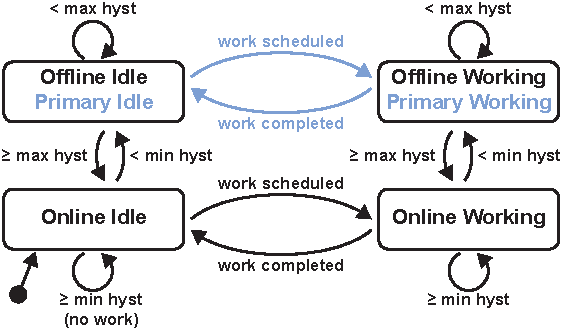
\includegraphics[width=\columnwidth]{figs/capacity/model_state_machine}
    \caption{\normalfont Model state machine.
    A modeled device can be in one of four states: \textsf{Offline Idle},
    \textsf{Online Idle}, \textsf{Online Working}, and \textsf{Offline
    Working}. When a device is \textsf{Offline Idle}, it has run out of energy
    and is off. If a device is \textsf{Online
    Idle}, it is on and in deep sleep, ready to perform work if triggered. If
    triggered, a device moves to \textsf{Online Working}, where it performs a
    portion of a work event.  If a workload is atomic, workload events
    \textit{must} be completed in one \textsf{Online Working} step, without any
    transitions to an offline state.  \textsf{Offline Working} means that while
    working on a non-atomic task, the device ran out of energy, checkpointed,
    and is waiting to harvest more and resume its task.  For devices
    configured with a primary-cell, \textsf{Offline Idle} and \textsf{Offline
    Working} become \textsf{\textcolor{primary-blue}{Primary Idle}} and
    \textsf{\textcolor{primary-blue}{Primary Working}} respectively.  In these
    states, outgoing energy is charged against the primary-cell and the device
    remains online and able to perform work for the life of the primary-cell.
    %State transitions are determined by incoming energy, the state of charge of
    %the secondary storage, and the generated work schedule from workload
    %parameters.
    }
\end{definefigure}

\section{\name Implementation}
\label{sec:impl:permamote}

%We discuss the implementation of both the model used to generate the results
%of \cref{sec:store} and \cref{sec:primary}, and the \name hardware that
%is based on these results. All of our hardware and software will be made
%\textbf{open source} for use by other researchers.


\begin{definetable}{tab:components}
    \begin{threeparttable}
    \centering
    \scriptsize
        \centering
        \scriptsize
        \begin{tabular}{l | l | c | c}
            Component                           &  Function                     & Active Power          & Idle Power \\\hline
            \multirow{2}{*}{Nordic NRF52840}    & Processor                     & 56\,\uA/MHz           & 940\,nA\,\tnote{a}  \\
                                                & Radio                         & 5.2\,mA @ 0\,dbm      & \textemdash\,\tnote{a}\\
            Ambiq AB1815-T3                     & Real time clock               & 55\,nA                & N/A\,\tnote{b}  \\
            ST Micro LIS2DW12                   & Accelerometer                 & 1\,uA @ 12.5\,Hz      & 50\,nA  \\
            Maxim MAX44009                      & Light sensor                  & 650\,nA               & N/A\,\tnote{b}  \\
            Intersil ISL29125                   & Color sensor                  & 56\,\uA               & 500\,nA  \\
            Silicon Labs SI7021                 & Humidty sensor& 1.5\,\uA @ 1\,Hz      & 60\,nA  \\
            TE Connectivity MS5637              & Pressure sensor               & 0.6 - 5\,\uA @ 1\,Hz  & 10\,nA  \\
            Panasonic EKMB11011                 & PIR Occupancy                 & 100\,\uA              & 1\,uA  \\
        \end{tabular}
    \end{threeparttable}
    \begin{tablenotes}[para]
    \scriptsize
    \item[a] Sleep current for both processor and radio.
    \item[b] No shutdown or idle mode.
    \end{tablenotes}
    \caption{
    \normalfont
    The components used in \name.
    These components are among the lowest power options available, and
    are even 2-4x lower power than those used on relatively recent
    systems such as BLEES, Flicker, Capybara, and Hamilton.
    }
    %Technology
    %scaling for embedded sensors, processors, and radios
    %has driven down the average power of a sensor node much closer to the
    %harvestable solar energy available in indoor lighting conditions. This allows
    %more systems to subsist or achieve extended lifetimes through energy harvesting.
\end{definetable}

\begin{definefigure}{fig:permamote}
    \centering
    \begin{subfigure}{0.7\columnwidth}
        \centering
        \includegraphics[width=\textwidth]{figs/capacity/arch}
        \caption{Harvesting and storage architecture}
    \end{subfigure}
    \begin{subfigure}{0.29\columnwidth}
        \centering
        \includegraphics[width=\textwidth,angle=90]{figs/capacity/permamote}
        \caption{Hardware}
    \end{subfigure}
    \caption{\normalfont The \name power supply architecture is informed by the
    findings in \cref{sec:store,sec:primary}. An
    LTO battery is recharged by a solar panel. When the battery is depleted,
    a primary-cell powers the system, providing reliability and avoiding
    intermittency.
    }
    %We believe this platform will run for 6-36 years for common
    %sensing tasks and indoor lighting conditions before the death of
    %the primary-cell. Even after the primary-cell expires,
    %the sensor node could continue to run intermittently on harvested energy.
\end{definefigure}

We implement the design principals discussed in \cref{sec:store,sec:primary}
in a new sensor called \name. The \name sensing platform
integrates a processor, BLE/802.15.4 radio, and various environmental, lighting,
and occupancy sensors. A picture
and system diagram of \name is shown in \cref{fig:permamote}. All hardware
and software for the platform is open source\footnote{\url{https://github.com/lab11/permamote/tree/master/hardware/permamote}}.\\

\vspace{-6pt}
\noindent
\textbf{Energy Harvesting and Storage.}
\name is powered by an energy harvesting front end that realizes the benefits
of using batteries. It uses the TI BQ25505 energy harvesting IC, which
harvests energy while monitoring both
rechargeable and backup energy stores,
switching between them at user-configurable voltages~\cite{bq25505}. A
20\,mAh (48\,mWh) LTO battery is charged by an 10.9\,cm\textsuperscript{2} amorphous
silicon solar panel~\cite{LTODatasheet, LTODatasheet2}. We limit the apparent
capacity of this battery to ensure
longer cycle lifetime as described in \cref{sec:battery}, but still have 24\,mWh of
energy storage, more than the capacity required to achieve the reliability and energy utilization
improvements described in \cref{sec:store}. For the backup energy
store, \name uses lithium primary-cells which can be configured to either one or two CR2032 coin
cells or a CR123A cell.
%Primary-cells provide 3-13x more density and 2-12x less
%leakage than a secondary-cell.
%making them more desirable than a single,
%large, pre-charged secondary-cell as the backup store~\cite{LTODatasheet,primary2032, primarycr123a}.
The output of the active battery
is boosted by a MAX17222 regulator, which features high conversion efficiency
(>90\%) at low output currents and operates down to 400\,mV~\cite{max17222}.\\
%We have the ability to monitor harvesting and system currents using
%the iCount method by sensing the voltage of
%the inductor used by the BQ25505 and MAX17222~\cite{duttaEnergy08}. The processor
%is also capable of gating all sensors from the main power supply to save
%power.\\

\vspace{-6pt}
\noindent
\textbf{Processor, Radio and Sensor Selection.}
In designing \name, we search for the newest and lowest power components.
%We feel that it may
To benefit other
platform builders, we document our component selections
along with their key performance metrics. A summary of these
components can be found in \cref{tab:components}.

We note our choice of the Nordic NRF52840 MCU over the more commonly used MSP430FR series
because of its higher efficiency in active mode while offering comparable sleep currents.
Specifically, it only draws 56\,\uA/MHz compared to over 100\,uA/MHz
for the MSP430. Unlike intermittent systems,
we do not rely on the FRAM present on the MSP430FR series chips. While
slightly more efficient
processors and radios exist than those found in the NRF52840,
we value the simplicity of an SoC-based design. \\

\vspace{-6pt}
\noindent
\textbf{Energy Benchmarks}.
The data presented in \cref{tab:components} are benchmarks taken
on the \name platform. We find that a BLE advertisement at 0\,dbm consumes
86\,\uJ and that sampling both light and color sensors and transmitting
them in a BLE advertisement consumes 586\,\uJ. Additionally, the entire system, including
the energy harvesting front end, consumes only 5.0\,\uW in deep sleep with RAM
retained and all sensors powered off. We use the energy numbers from \name as a basis
for our workloads to fairly compare against prior energy storage architectures.
%\subsection{Numerical Model}
%\label{impl:model}
%
%We develop a numerical model that simulates the behavior of energy harvesting
%systems in indoor environments. For this work, we've primarily focused on solar
%energy input, and have tailored the model to use solar energy traces. As
%mentioned, we use the Columbia EnHANTs irradiance traces
%\cite{margolies2015energy}. We process the traces, filling the few periods of
%missing data by copying from a week prior.
%
%The model operates at second granularity, and at each
%step, the amount of incoming energy is calculated based on the input irradiance
%and solar panel configuration. If the device has enough energy to turn on
%and perform the task from the specified workload it does so. If there is
%energy to spare after the task, the device will enter a low power sleep state.
%The model tallies the amount of successful and unsuccessful events that it
%was expected to complete, as well as the percentage of energy used out
%the energy that was available from the harvesting source. To estimate
%lifetime, the model attempts tasks for the totality of solar irradiance
%data present, then extrapolates primary-cell discharge to find its lifetime
%at empty. The one second granularity imposes some limitations, however
%we find that sensor node workloads are rarely more intensive.
%
%If the secondary store is not at capacity
%this incoming energy is stored
%
%If the device is online, it attempts to turn on
%if it has enough energy to do so, otherwise it remains offline and continues to
%fail performing its workload.  If the device is on, it perform tasks from its
%workload. It prioritizes using the energy from its rechargeable store, and if
%depleted, will either go offline or use energy from its primary-cell, if
%available. If it has energy to spare, it enters a low power sleep state. The
%model tallies the amount of successful and unsuccessful events that it was
%expected to complete, as well as the percentage of energy it used out of how
%much was available from the irradiance source. It also performs a linear fit on
%the primary state of charge to estimate lifetime, if applicable to the
%simulated device's configuration.
%
%This
%granularity also limits that of workloads to a second, but we argue
%that realistic sensor workloads are rarely more intensive \hl{cite}.


\placefigure[t]{fig:permamote}


\section{Model Evaluation}
\label{sec:eval}
To evaluate the model, we perform a three-month-long deployment in a partially sunlit room
using i) a primary-cell only system, ii) an intermittent, capacitor-only system, and iii) \name, our
system that features both a secondary and primary-cell. We model these
systems over the same period and compare the availability of \name to the
intermittent system.

\subsection{Model Analysis}
\label{sec:eval:model}
We analyze the deployment of these systems
%in a partially sunlit room for three months
and compare their behavior to our
model's predictions: i) ten CR2032 primary-cell only devices, ii) an
intermittent system configured with just 500\textmu F of capacitance (about
0.36\,\textmu Wh at 2.2\,V), and iii) \name, configured with a 20\,mAh
(48\,mWh) secondary-cell, half of which is usable, and a CR2032 backup.  The
primary-cell only device performs environmental sensing over BLE every second.
The intermittent system  sends a beacon as soon as its capacitor bank is full.
When its energy is depleted, it powers off and charges
again. \name is running the ``sense and send'' workload that we described in
\cref{sec:overview}, and sends illuminance measurements every second. This
workload stresses the model and requires more charge and discharge cycles.  We
use \name illuminance readings to estimate irradiance using the same scaling factors used by
Yerva et al.~\cite{yervaGrafting12}, and use these traces as
model input.\\

\vspace{-6pt}
\noindent
\textbf{Primary-Cell Only.}
We model the workload of the primary-cell system and produce estimates for
lifetime.  Our model predicts the platform lifetime
to be 58 days.  We find that the average lifetime of the 10 devices is 61 days.
%,
%from initial deployment to energy depletion, is 61 days.
\\

\vspace{-6pt}
\noindent
\textbf{Intermittent.}
We model the number of packets sent each hour by the
intermittent system over a three week period, and compare against the results of an actual device in
\cref{fig:eval:pkt}.
The average daily error of the model versus our results is 15\%, with a standard deviation of
17\%. This error can attributed to two primary sources. Illuminance is measured
close to, but not exactly at the solar panel of the test device. Occasional
direct sunbeams, like that experienced on day 16, can illuminate the solar
panel but not the sensor, or vice versa. This
results in a substantial over or underestimate of available light. In addition
to inaccurate light measurements, we introduce error through our estimation of
irradiance. We measure illuminance
instead of irradiance, and must resort to a piecewise linear estimation, when
in reality the relationship is not well defined and non-linear when considering
different light sources. In the case of our estimation, results
indicate that the model consistently underestimates high irradiance measurements.\\
\placefigure{tab:components}
\placefigure[t]{fig:evalcmp}

\vspace{-6pt}
\noindent
\textbf{Secondary and Primary-Cell.}
We compare our model's predicted state of charge to a deployed \name over a seven
day period in \cref{fig:eval:soc}. We estimate state of charge from the reported secondary-cell
voltage,
%,
%and measured voltage
%curves of the installed 20\,mAh battery
and irradiance from
lux measurements. In this figure, the state of
charge cycles between configured battery hysteresis limits, as the workload is
too intense to be sustained by energy harvesting alone.
%and the Permamote must
%use energy from its primary cell.
Flat and upward slopes of the curve represent the
device in hysteresis, using the primary battery to perform its workload. Upper slopes
indicate the secondary cell is charging from harvested energy.
Downward slopes indicate the device is out of hysteresis and is using harvested
energy stored in its secondary battery to perform its workload.
%The device is
%charging and in
%hysteresis during upward
%slopes.
The shaded ``nighttime'' regions are not uniform, as the
deployment environment is occupied by graduate students that occasionally work
late hours or forget to turn off the lights.  The model correctly predicts the
cycling
behavior of the deployed device for two days, but deviates
during the third day. The model predicts that the device would charge above the upper
hysteresis limit and begin supplying energy from the secondary-cell before the
test device actually does.  This inaccuracy, like that of the last of
experiment, is partially due to our inexact estimation of irradiance.  In
addition, real device hysteresis limits are set using resistor networks.  The
resistors used have 1-5\% tolerance, and are susceptible to temperature
changes, which introduces dynamic errors that is not accounted for in our model.
Even though the predicted state of charge deviates after two days, the length
and frequency of periods in which harvested energy is stored and used %in the secondary-cell
are identical to our experimental measurements.
%While our model correctly predicts cycling timing and frequency, it appears the
%state of charge  does not quite match that of the measurements.  This is
%because the voltage measured is not the open circuit voltage, and is affected
%by voltage droop due to the applied system load as well as inflated charging
%voltage from the energy harvesting front end.  Ignoring these effects, the
%cycling of the model's prediction is closely synchronized with the estimated
%state of charge.
%We compare the model's predicted
%state of charge over time to the outputs of systems we
%have deployed. For energy harvesting systems we collect lux measurements
%throughout the deployment and convert lux to irradiance based on the
%data collected in Yerva et al.~\cite{yervaGrafting12}. \\
%\vspace{-6pt}
%\noindent
%\textbf{Permamote.}\\
\subsection{\name Performance}
\placefigure[t]{fig:eval}
\label{sec:eval:permamote}
%In addition to evaluating our model,
We also compare the performance of the
deployed intermittent system and \name. In \cref{fig:evalcmp}, we show the
number of packets sent per hour for two days. \name sends data every
second, while the intermittent system sends as fast as possible. \name is
able to collect and send its data continuously, while the
intermittent system is limited to sending only during the day. This
demonstrates the increased availability afforded by increasing secondary
capacity and including a backup energy store.

We also use our model to explore the estimated performance of \name
compared to prior systems.
To isolate the analysis to just power supply types and sizing, we assume each
system uses the same low-power hardware and is performing the same workload.
The results of this modeling are shown in \cref{tab:related}. Our model estimates that
\name can expect several decades of 100\% reliable lifetime when configured as
it was deployed for this evaluation, albeit configured with a less intense workload.
%While the workload used with \name is not
%sustainable for the multi-decade lifetimes we are targeting, it still
%exemplifies the increase in reliability afforded by including a primary-cell.


\begin{definefigure}{fig:eval}
  \centering
  \begin{subfigure}{\columnwidth}
    \centering
    \includegraphics[width=\linewidth]{figs/capacity/experiment_pkt/exp_vs_sim_pkt}
    \caption{Intermittent Node}
    \label{fig:eval:pkt}
  \end{subfigure}\\%\hspace{0.5cm}
  \begin{subfigure}{\columnwidth}
    \centering
    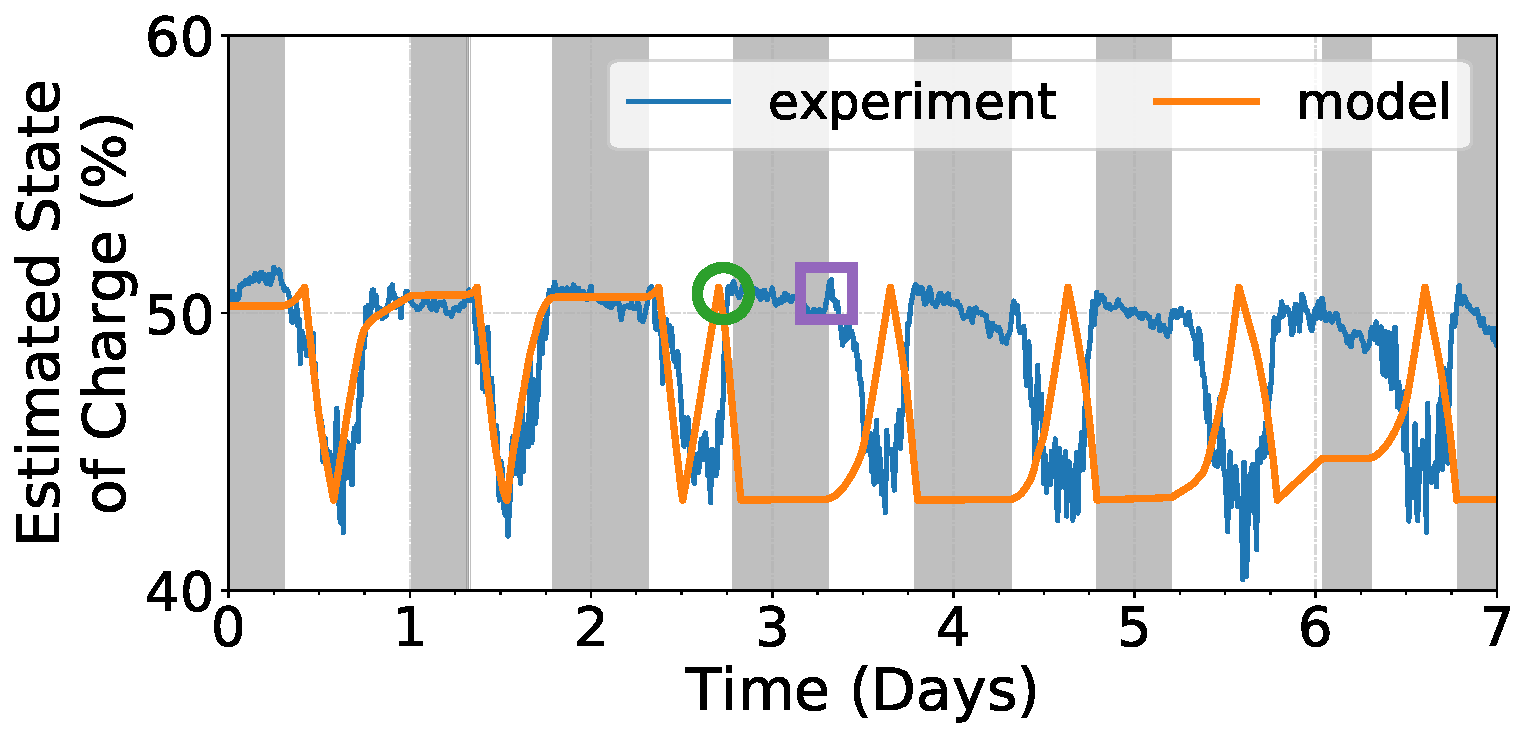
\includegraphics[width=\linewidth]{figs/capacity/experiment_soc/exp_vs_sim_soc}
    \caption{Permamote}
    \label{fig:eval:soc}
  \end{subfigure}
    \caption{Model comparison to deployed hardware.
    \normalfont
    Data from a three month deployment of two systems is used to verify our model.
    (a) We use three weeks of lux measurements %from a month-long deployment
    to estimate irradiance and model the number of packets transmitted by an
    intermittent node. Average daily error is 15\%, with a standard deviation
    of 17\%. (b) We model and measure a \name's state of charge while running a
    ``sense and send'' workload with a 1\,s period for a week, beginning at
    midnight on the first day. Secondary charging hysteresis
    limits of the devices are set at 51\% and 43\%. Shaded regions
    represent periods of low harvestable potential
    (<\,15\,\textmu W/cm\textsuperscript{2}),
    i.e. nighttime. For the first two days, model predictions
    closely track the experimental measurements. Errors
    in hysteresis and irradiance estimation cause the model to reach its upper
    hysteresis sooner than the experiment does, annotated by the
    \textbf{\textcolor{fig-green}{green circle}}. In actuality, the device
    exits charging hysteresis at the peak marked with the
    \textbf{\textcolor{fig-purple}{purple square}}.
    More importantly, the
    frequency and length of periods spent using harvested
    energy collected in the secondary-cell (downward slopes) are identical.
    %For the intermittent node we see our model
    %underestimate the number of transmitted packets by 10-20\% except for the
    %first day which predicts significantly more packets.  We believe this error
    %is primarily due to a piecewise linear estimation of irradiance from our
    %collected illuminance data, when in reality the relationship is complex and
    %non-linear.  For (b) we estimate the state of charge of \name
    %based on the secondary
    %cell voltage. Differences between the estimated state of charge and the
    %modeled state of charge are primarily due to inflated voltage during
    %charging and voltage droop and bounce back when \name
    %draws current from the secondary-cell.
    %Even though estimated state of
    %charge is not accurate due to this voltage swing, it is clear that the
    %timing of charge and discharge aligns between the model and the
    %experimental data.
    }
\end{definefigure}

\begin{definefigure}{fig:evalcmp}
    \centering
    \includegraphics[width=\linewidth]{figs/capacity/experiment_sys_compare/exp_packets_recv}
    \caption{
      \normalfont
        Packets received over two days.
      This figure compares the reliability of an
      intermittent design and \name. \name sends a packet every second and does
      so without fail, while the intermittent system is only able to send when
      light is available.
      %This results in periods at night where the
      %intermittent device does not harvest enough energy to sustain operation.
      }
\end{definefigure}
\placefigure{tab:related}


\section{Summary}

\chapter{A Quantitative Evaluation of Energy Storage}
\label{chap:battery}

From the previous chapter, I have identified the value of properly sizing energy capacity in an energy harvesting design to increase energy capture and system reliability. 
Many modern energy harvesting sensor designs have utilized capacitors in their designs, which severely limit energy capacity.
Many modern platforms are attempting to push the energy bounds of sensing, computation and networking, and have begun incorporating supercapacitors to provide the necessary energy to make certain applications feasible~\cite{nardello2019camaroptera}.
These decisions are made despite the obvious option for energy capacity: batteries.
%Due to an increased need for energy storage to enable more advanced sensing and processing, the majority of modern batteryless research energy harvesting platforms utilize supercapacitors instead of tantalum or ceramic capacitors due to their superior energy density.
These designers have eschewed batteries as an option, despite their vastly superior energy density, dismissing them qualitatively as 
bulky~\cite{yervaGrafting12, hester2017future, hesterTragedy15, luciaIntermittent17, hesterFlicker17, hesterTimely17, colinReconfigurable18, yildirim2018ink, nardello2019camaroptera, geissdoerfer2019shepherd, majid2020continuous, shukla2019skinnypower},
inefficient~\cite{yervaGrafting12, luciaIntermittent17, nardello2019camaroptera, shukla2019skinnypower},
expensive~\cite{hester2017future, hesterTragedy15, hesterFlicker17, hesterTimely17, yildirim2018ink, majid2020continuous},
short-lived~\cite{hester2017future, hesterFlicker17, hesterTimely17, colinReconfigurable18, luciaIntermittent17, yervaGrafting12, shukla2019skinnypower, geissdoerfer2019shepherd, nardello2019camaroptera, fraternali2020ember, majid2020continuous}.
%high-maintenance~\cite{hesterNew17, hesterTragedy15, hesterFlicker17, hesterTimely17, colinReconfigurable18, luciaIntermittent17},
temperature-sensitive~\cite{hester2017future, hesterFlicker17, hesterTimely17, luciaIntermittent17, colinReconfigurable18},
%difficult to monitor~\cite{hesterNew17, hesterTragedy15, hesterFlicker17, hesterTimely17, colinReconfigurable18, luciaIntermittent17},
%fragile~\cite{hesterNew17, hesterTragedy15, hesterFlicker17, hesterTimely17},
and dangerous~\cite{hester2017future, hesterFlicker17, hesterTimely17,  yildirim2018ink, geissdoerfer2019shepherd, majid2020continuous}. 
%These qualitative claims against batteries were valid when considering some of the first available rechargeable batteries. 

In this chapter, I reexamine each of these arguments with respect to modern capacitor, supercapacitor, and battery technology. 
While the early battery design of one or two decades ago were certainly guilty of many of the complaints against them, new 
battery electrode materials and improved lithium-ion manufacturing processes have produced appealing options for miniature energy storage 
that do not possess the same negative qualities as older battery technology. 
%These new batteries still possess orders of magnitude more energy density than capacitors and supercapacitors.
New battery technology paired with newly available low power energy harvesting and battery management ICs~\cite{bq25505,adp5091} enables the design of high-capacity energy harvesting systems.
Despite improvements, batteries still underperform in some metrics compared to supercapacitors, but these deficiencies are likely inconsequential for the majority of wireless sensor applications, and the substantial increase in energy capacity outweighs any detracting trade-offs.\\

\begin{landscape}
\placefigure{tab:battery:cost}
\end{landscape}

\section{Energy Storage Technology}
\label{sec:battery-new}

I summarize the notable characteristics of various examples of capacitors, supercapacitors, and batteries in \cref{tab:battery:cost}. Many of the capacitors and supercapacitors in this table were chosen based on their inclusion in some contemporary batteryless platforms, including the Solar Monjolo~\cite{campbellEnergy14}, Flicker~\cite{hesterFlicker17}, Capybara~\cite{colinReconfigurable18}, and Camaroptera~\cite{nardello2019camaroptera}.
The selected batteries represent some of the smallest lithium-based cells that are commercially available. 
This section serves to explain the characteristics of various possible energy storage technologies for low power energy harvesting applications, as a prelude to deeper dives on particular aspects and comparisons.

\subsection{Ceramic and Tantalum Capacitors}
Along with chip resistors, the multilayer ceramic capacitor (MLCC) is the most widely used passive component in modern electronics. MLCCs are essentially a parallel connection of many cearamic plate capacitors, packaged in a small form factor~\cite{pan2010brief}. Traditionally, MLCCs are used for two applications: resonant circuits and filters and power supply bypass and decoupling~\cite{pan2010brief}. With sufficient capacitance, MLCC capacitors meant for power supply decoupling can act as the sole energy storage in a system~\cite{hesterFlicker17,yervaGrafting12,campbellEnergy14}. However, the energy storage and density of MLCC components is limited, and is often only enough to support a single small operation, like operating a sensor and transmitting the results over a radio. Similarly, tantalum capacitors are often used for power supply bypass and decoupling. Tantalum capacitors consist of a tantalum metal anode and a solid electrolyte as a cathode, separated by a solid dielectric~\cite{gill1994basic}. They generally provide more capacitance per volume than MLCCs, but are polar and have worse efficiency.
Tantalum capacitors also do not exhibit any aging effects, whereas MLCCs experience slight capacitance change over long periods of time~\cite{kemetUpdate}.
Compared to batteries and supercapacitors, MLCC and tantalum capacitors provide infinitely longer lifetimes and higher power density, but are severely limited in energy capacity and density.

\subsection{Supercapacitors}
Electrochemical double layer capacitors (EDLC) are the most common type of supercapacitor, and are utilized in many batteryless platforms~\cite{colinReconfigurable18,libich2018supercapacitors,nardello2019camaroptera}.
Supercapacitors generally consist of electrodes separated by a liquid electrolyte, like batteries, however energy accumulation is through electrostatic interaction instead of chemical reactions~\cite{libich2018supercapacitors,vangari2013supercapacitors}.
EDLCs achieve significantly higher energy density than MLCC and tantalum capacitors due to their large effective surface area and very small charge separation distances. Supercapacitors are also durable and long-lived, capable of millions of cycles~\cite{libich2018supercapacitors}. 
supercapacitors excel in high power, high cycling applications, where large amounts of charge must be stored and provided quickly, at a high frequency.
However, they offer lower power densities due to higher internal resistance compared to MLCC and tantalum capacitors~\cite{vangari2013supercapacitors}. 

\subsection{Li-ion}
Lithium-ion batteries encompass all batteries that utilize lithium ions for charge transfer. These batteries are well known for their superior energy density, and are used in small wireless and portable consumer electronics as well as in large multi-cell configurations in electric vehicles.
Like all batteries, Li-ion batteries consist of two oppositely charged electrodes separated by an electrolyte. The electrodes consist of a negatively charged anode and positively charged cathode. During discharge, Li\textsuperscript{-} ions move from the anode through the electrolyte to the cathode, and during charge they move from the cathode to the anode.
Lithium polymer (Lipo) batteries, most commonly used in consumer electronics, utilize a dry or gel electrolyte, while coin cells or cylindrical Li-ion cells utilize a liquid electrolyte. 

There are many different types of li-ion batteries, utilizing different anode, cathode, and electrolyte materials. Most modern Li-ion cells primarily utilize graphite as an anode material, and lithium nickel manganese cobalt oxide
(LiNi\textsubscript{0.33}Mn\textsubscript{0.33}Co\textsubscript{0.33}O\textsubscript{2} or NMC for short) as a cathode material~\cite{nitta2015li}.
These cells offer a nominal voltage of 3.7\si{\volt}, high energy density, and long lifetimes. 
The choice of NMC provides several benefits over earlier designs that utilize 
LiCoO\textsubscript{2} (LCO) or LiMn\textsubscript{2}O\textsubscript{4} (LMO) for cathode materials.
LCO lithium batteries are notorious for their thermal instability and fast capacity fade at high current rates or deep cycling~\cite{nitta2015li}. 
Cobalt is also a toxic and expensive metal to produce. 
LMO lithium batteries are cheaper, have higher power density, and have significantly better thermal stability than LCO cells, but have lower energy density and still have poor cycling stability, especially at higher temperatures~\cite{nitta2015li}.
The combination of nickel, manganese, and cobalt in NMC cathodes results in higher structural stability, longer lifetimes, and less reliance on expensive transition metals~\cite{nitta2015li}. 

Batteries that utilize LCO cathodes have the propensity to ignite or explode due to thermal runaway when stressed thermally, mechanically, or electrically~\cite{doughty2012general}. This is primarily due to the cathodes releasing oxygen at high temperatures, which start an exothermic reaction with the organic parts of the cell~\cite{doughty2012general, nitta2015li}. Like LCO, the newer NMC cathode material is still susceptible to thermal runaway with abuse, however the peak magnitude of self-heating on runaway is an order of magnitude less than that of LCO, and onset is delayed and begins at a higher temperature~\cite{doughty2012general}.
Batteries with LMO cathodes are safer than both LCO and NMC, but have poor cycle cycling lifetime which has limited the technology's commercialization. 

\subsection{Lithium Iron Phosphate}
Lithium iron phosphate  (LiFePO\textsubscript{4}, or LFP), is a more recently commercialized cathode material and stands to offer similar safety and power capability to LMO while offering long lifetimes similar to NMC~\cite{preger2020degradation, nitta2015li}.
Batteries that utilize LFP as a cathode material possess a lower nominal voltage (3.2\si{\volt}), and lower energy density than LCO and NMC batteries. However, LFP 
cathodes offer higher cycle stability and lifetime, have lower thermal sensitivity, and are cheaper to produce than cobalt and manganese-based cathodes~\cite{doughty2012general,nitta2015li,preger2020degradation}. LFP cells are also very safe compared to NMC and LCO cells. The only thermal runaway experienced by LFP batteries is dominated by reactions between the electrolyte and graphite anode, which decomposes at high temperatures~\cite{doughty2012general}. 

\subsection{Lithium Titanate Oxide}
Perhaps the most promising replacement for graphite anodes is lithium titanate oxide (Li\textsubscript{4}Ti\textsubscript{5}O\textsubscript{4}).
Lithium titanate oxide, abbreviated LTO, is usually paired with an LMO cathode, and sometimes an NMC cathode~\cite{nitta2015li, belharouakElectrochemistry11, sandhya2014lithium}. LTO offers superior thermal stability, high discharge/charge rates, and longer lifetimes compared to graphite. These improvements come at a cost of the more expensive titanium compound, and a lower energy density and nominal voltage (2.4\si{\volt})~\cite{nitta2015li,sandhya2014lithium}. Cells that incorporate LTO anodes are also extremely safe compared to those that use graphite~\cite{nitta2015li, belharouakElectrochemistry11, sandhya2014lithium}. Unlike graphite, LTO anodes do not produce Li dendrites after considerable cycling~\cite{nitta2015li}. This reduces the risk of inadvertent internal shorts and thermal runaway. LTO anodes also remain stable and do not break down at high temperatures~\cite{belharouakElectrochemistry11}.

\subsection{Solid-state}
All cylindrical or pouch Li-ion batteries employ a liquid or gel electrolyte of lithium salts dissolved in an organic, non-aqueous solvent~\cite{doughty2012general}. Liquid electrolyte requires specific packaging to prevent leakage, and an internal separator to prevent shorts between the electrodes. This limits the miniaturization of Li-ion batteries, as this packaging is increasingly difficult to manufacture at smaller sizes. This results in smaller batteries that have uncharacteristically high internal resistance and lower energy density compared to larger cells with the same chemistry.
The organic solvent used in liquid and gel electrolytes also can react exothermically with any oxygen released upon the breakdown of electrode material and cause thermal runaway. In addition to developing new anode and cathode materials to mitigate this, researchers and companies have also begun experimenting with replacing the non-solid electrolyte non-reactive alternatives. Solid-state batteries are safer, due to the use of non-reactive solid electrolytes, come in smaller packages, offer longer lifetimes, and have very low self-discharge~\cite{kim2015review}. However, solid-state batteries generally have limited energy and power density and high internal resistance compared to aqueous Li-ion cells. Solid-state batteries are also currently expensive to manufacture, and their commercial viability has been limited~\cite{kim2015review}.

\subsection{Summary}
Capacitors possess superior power density and have functionally infinite lifetimes, but can only store minute amounts of energy. Supercapacitors provide one to two orders of magnitude more energy density than MLCC and tantalum capacitors, at the cost of reduced power density, and more limited lifetimes. By contrast, batteries offer one to two orders of magnitude more energy density than supercapacitors. However, batteries do have limited lifetimes based on cycle counts, are more temperature sensitive, and some can be dangerous if mishandled. 

In the rest of this chapter, I seek to compare these technologies in more depth. The following sections directly analyze each of the high-level qualitative arguments that "batteryless" platform designers have leveled against batteries. Namely, that they are bulky, inefficient, expensive, short-lived, temperature-sensitive, and dangerous. 


\section{Volume and Density}
\label{sec:battery:density}
Arguments that deride batteries as bulky are likely directly comparing the size of a small battery to that of single tantalum or ceramic capacitor, without considering energy and power density. Modern, commercially available miniature batteries are comparable in volume to many supercapacitors, and even a banked combination of ceramic and tantalum capacitors, while offering substantially more energy density and an acceptable power density. In this section, I explore the "bulkiness" of capacitors, supercapacitors, and batteries in the context of energy and power density. Here, I am considering volumetric density (\si[per-mode=symbol]{\Wh\per\liter}  and  \si[per-mode=symbol]{\watt\per\liter}) instead of specific energy and power (\si[per-mode=symbol]{\Wh\per\kilo\gram} and  \si[per-mode=symbol]{\watt\per\kilo\gram}, respectively) to better compare the volume of these energy storage options. The energy density and power density of various capacitors, supercapacitors, and batteries are directly compared in \cref{fig:battery:ragone}.

\placefigure{fig:battery:ragone}

\subsection{Energy Density}
Energy density should be the primary consideration for energy harvesting power supply design to maximize energy capacity while simultaneously minimizing volume. 
The energy stored in a capacitor is calculated in one of two ways:

$$E_{eff_{cap}} = \frac{1}{2} C (V^2 - V_{min}^2)$$
$$E_{total_{cap}} = \frac{1}{2} C V^2$$

\noindent Where $E_{eff}$ and $E_{total}$ is the effective and total energy stored in a capacitor, respectively. These amounts are defined by the capacitor's capacitance $C$, and the applied voltage $V$, and the minimum voltage $V_{min}$. Usually $V_{min}$ represents the minimum to do something useful. Often this is the minimum open circuit voltage to cold start a boost regulator, between 400\si{\milli\volt} to 600\si{\milli\volt}~\cite{adp5091,bq25505,max17222}. 
For simplicity, I use $E_{total}$ to determine energy capacity and density. For most capacitors, the unusable energy represented by $E_{eff_{cap}}$ is negligible compared to the total energy. Likewise, energy stored in a battery is estimated as follows:

$$E_{bat} \approx Q V_{nom}$$

\noindent Where $Q$ is the charge capacity (often denoted in terms of \si{\Ah}) and $V_{nom}$ is the battery's nominal voltage. Nominal voltage represents an average of the battery's voltage curve over the course of a charge/discharge cycle. The nominal voltage and capacity of a battery are provided by the manufacturer and are almost always included in a datasheet.

A selection of capacitor, supercapacitor, and battery energy capacities and densities are summarized in \cref{tab:battery:cost}, and their energy density is compared in \cref{fig:battery:ragone}. Among this selection, small batteries are 50-1000x more energy dense than supercapacitors and three to five orders of magnitude more dense than ceramic and tantalum capacitors. Li-ion and LiPo batteries are the most energy dense among all options. Solid-state batteries are an order of magnitude less energy dense than those with aqueous electrolytes, but still an order of magnitude more dense than supercapacitors. 

Several of these capacitors, supercapacitors and batteries are shown visually in \cref{fig:battery:sizes}.
The capacitor and supercapacitor configurations are based on examples from batteryless platform designs described in the literature~\cite{hesterFlicker17, campbellEnergy14,colinReconfigurable18}.
The batteries shown in \cref{fig:battery:sizes} are
as small as 88\si{\milli\meter\cubed}, and resemble small through-hole
capacitors and coin cells. Battery \textbf{(b)} is smaller in volume than many of the capacitor
configurations presented in the literature, only outdone by systems like Flicker \textbf{(a)} which utilize only a few ceramic capacitors~\cite{hesterFlicker17}.
This small LTO battery offers 3.7x 
more energy storage and 50x more energy density than the largest supercapacitor presented (\textbf{h}). When considering the size of other components in the system, most notably the harvester (solar panel, thermocouple, or piezoelectric device), the combination of ICs, and large sensors like a PIR motion sensor, the size of small rechargeable batteries is inconsequential. 
To my knowledge, the Michigan Micro Mote is the smallest energy harvesting system, occupying a volume on the order of a single ceramic capacitor~\cite{lee13modular}. Despite its small size, it utilizes a thin film solid-state lithium battery for energy storage due to its superior energy density over any capacitor or supercapacitor option.
When one considers energy density instead of purely volume, capacitors and supercapacitors are significantly more bulky than batteries.

\placefigure{fig:battery:sizes}

\subsection{Power Density}
In addition to energy density, power density is also an important metric to consider for a design. 
Common wireless sensor workloads are characterized by very low sleep currents punctuated by infrequent pulses of high current, usually a radio transmission. Energy storage must provide sufficient peak power to drive these short pulses, but largely, these applications require low continuous power. The maximum peak power is largely dependent on equivalent series resistance (ESR) of the storage device, represented by an internal series resistance to the capacitor or battery cell. 
Internal resistance for both supercapacitors and batteries is temperature and age dependent. Both storage elements experience increased ESR at temperature extremes, and experience increased ESR as they age.
The internal resistance of capacitors and supercapacitors is also frequency dependent, and usually reported for 1\si{\kilo\hertz}. This value is generally related inversely with frequency for frequencies below the capacitor's self-resonance~\cite{murataESRArticle}. For the relatively low frequency of charge/discharge cycles characteristic of energy harvesting devices, actual ESR is likely higher than reported for supercapacitors.

Internal capacitor, supercapacitor, and battery resistance incurs a voltage drop over this resistance which is especially noticeable and detrimental during high  current loads.
Ceramic and tantalum capacitors have negligible ESR and incomparably high power density, so I focus on comparing the power density of supercapacitors and batteries.
There are two different metrics for quantifying power output of supercapacitors and batteries. The first is effective power $P_{eff}$, and represents the maximum sustainable continuous power that can be provided. The second is peak power $P_{max}$ and represents the maximum possible current that can be provided in short pulses. These metrics are defined differently for supercapacitors and batteries. For a supercapacitor, power output is defined as follows~\cite{IEC62391}:

$$P_{eff_{sc}} = \frac{1}{8} \frac{V^2}{R_i}$$
$$P_{max_{sc}} = \frac{1}{4} \frac{V^2}{R_i}$$

\noindent Where $V$ is the voltage applied to the capacitor, and $R_i$ is the internal resistance, or ESR. For batteries, these metrics are defined as follows:

$$P_{eff_{bat}} = I_{cont} V_{nom}$$
$$P_{max_{bat}} = I_{max} V_{nom}$$

\noindent Where $I_{cont}$ and $I_{max}$ are the battery's rated continuous and peak pulsed current respectively. These metrics are provided by the battery manufacturer and often included in the battery datasheet. The continuous and peak currents are often defined in terms of the C-rate, or a proportion of the rated capacity (in units of \si{\Ah}). For example, the 1C rate of a 100\si{\milli\Ah} battery is 100\si{\milli\ampere}, and the 2C rate is 200\si{\milli\ampere}. 
Continuously charging and discharging a battery beyond its normal rate will result in cycles that deliver less energy than rated, and eventually damage to the cell resulting in capacity fading. 
For sake of comparison, I use $P_{eff}$ in \cref{tab:battery:cost} for batteries and supercapacitors, as it is a more conservative measure of the energy storage power capability. 

Among the supercapacitors and batteries featured in \cref{tab:battery:cost}, supercapacitors provide 10-400x higher power density over batteries. 
However, one supercapacitor outlier provides the least power density of all options. Like energy density, power density is also directly compared in \cref{fig:battery:ragone}.
Despite their superior power density, most applications do not require the higher power density afforded by supercapacitors. 
It is hard to imagine a \textit{low power} energy harvesting application that must source more than a few to a few hundred \si{\milli\ampere} at 3\si{\volt} infrequently, never mind continuously. 
Solid-state batteries are more power limited than other battery types. Despite their low energy capacity they are able to supply high C-rates, between 15-50C. This corresponds to currents on the order of 10\si{\milli\ampere}.
Conventional Li-ion and LiPo cells can generally source 1C continuously. The smallest Li-ion cell listed in \cref{tab:battery:cost} can provide 11\si{\milli\ampere} continuously, and the largest can provide 80\si{\milli\ampere}. The LiPo cell presented can supply 40\si{\milli\ampere} continuously. 
Small LTO and LFP cells are capable of very high C-rates, often between 20-40C for LTOs, and 10-20C for LFP~\cite{lifepo4Datasheet,LTODatasheet,LTODatasheet2}.
The smaller LTO battery listed in \cref{tab:battery:cost} is able to source 18\si{\milli\ampere}, while the larger LTO and LFP cells can source between 400-700\si{\milli\ampere} continuously. 
This power capability is more than sufficient for the majority of applications, either indoors with PANs, or outdoors, with cellular or LPWANs~\cite{nrf52840,ghena2019challenge}.

Another consideration for power capability and ESR is the effect of voltage drops during high power loads. If a voltage drop is sufficiently large, it can drop the supply to a level unusable by a voltage regulator or CMOS logic. This could effectively render part of the power storage unusable in an unpredictable manner. This effect is particularly detrimental for supercapacitors. While ESR is comparable between batteries and supercapacitors, the stability of provided voltage is not. Batteries provide a stable voltage curve centered around their nominal voltage, and voltage drops due to ESR can still result in a usable voltage even when almost empty. Supercapacitors, on the other hand, experience a (approximately) linear decrease in voltage with current until empty. This means that, depending on the load (in intensity and frequency), a large load and subsequent voltage drop could occur that causes a system brown-out, potentially corrupting state, or an unexpected reset. 


\section{Efficiency}
\label{sec:supercapvbattery}
At a high level, the efficiency of an energy storage element can be defined as the actual proportion of stored energy that is used to perform a desired task or application. Batteries have been derided as "inefficient" by batteryless platform designers, however
both supercapacitor and battery technology exhibit the same two phenomena that causes inefficiency, and generally to the same extent. 
The first phenomena is power dissipation over the internal resistance of the device. The second is self-discharge or leakage, which is represented by an internal parallel resistance to the capacitor or battery.
This section seeks to quantitatively compare these two sources of inefficiency for supercapacitors and batteries.

\subsection{Internal Resistance}
The power dissipated over the internal resistance, or ESR, of an energy storage element can be calculated as follows:

$$P_{i} = R_{i} I^2$$

\noindent Due to the squared relationship of power to current, high current loads, such as a radio transmission or long computation, are the primary cause of ESR power losses. The total power required to drive a load, including losses over internal resistance, can be defined as:

$$P_{total} = P_{l} + P_{i}$$
$$P_{total} =  I V + R_{i} I^2$$

\noindent Where $P_l$, $I$ and $V$ are the power, current, and voltage required to drive an intended load. Power inefficiency due to ESR can be very costly when considering high current loads.

With a subset of the capacitors and batteries mentioned in \cref{tab:battery:cost}, an 8\si{\milli\ampere} BLE
transmission from a steady 3\,V would incur less
than 0.03\% in resistive loss from a tantalum capacitor, a 2.1\% loss from the 1.8\si{\milli\Ah} LTO battery, and 6.3\% loss from the 7.5\si{\milli\farad} supercapacitor. A 130\si{\milli\ampere} LoRa transmission would incur a 0.43\%, 25\%, and 52\% overhead, respectively~\cite{ghena2019challenge}. These selections represent some of the worst performing examples in terms of ESR. 
For most supercapacitor and battery product lines, as they get smaller, capacitance and capacity decreases while ESR increases. When the surface area between cell electrodes decreases, this limits the flux of ions traveling between electrodes. This is manifested as an increased internal resistance.
This has traditionally been an issue for small Li-ion batteries. However, the recent commercialization of new manufacturing processes and new cathode and anode materials that increase electrode surface area has led to small form factors with lower ESR, on the order of 1-2\si{\ohm}~\cite{millibatNimbus}. Current solid-state battery technology still struggles with ESR, with values at or above 100\si{\ohm}~\cite{stEnfilm,tdkCeraCharge}.
In \cref{tab:battery:cost}, there are several batteries and supercapacitors that exhibit much lower ESR, on the order of 1\si{\ohm} or less, and are thus more efficient with high current loads. 
The 20\si{\milli\Ah} LTO battery is in the same product line as the 1.8\si{\milli\Ah} cell, but has 15x less ESR. This cell would only incur a 0.15\% and 2.3\% loss on the respective BLE and LoRa transmissions.
%For high current loads, it is very important to not only pick a storage element that can support the load, but one that also has a low internal resistance to energy wasted over the internal resistance. 
Generally, there are options for both supercapacitors and batteries that offer comparable ESR efficiency. %In this respect, batteries \textit{are not} inefficient.


\subsection{Self-Discharge}
In addition to an internal series resistance, capacitors and batteries both feature a non-ideal parallel resistance that causes a continuous self-discharge.
The self-discharge of supercapacitors and batteries is generally dependent on their size and temperature. Larger capacity/capacitance batteries and capacitors from the same product line will exhibit more self discharge than smaller ones. 

The batteries selected in \cref{tab:battery:cost} typically exhibit less than 500\si{\nano\ampere} self-discharge in standard environmental conditions. Solid-state batteries exhibit even less self discharge, at similar rates to capacitors. Notably, many types of Li-ion and LiPo batteries also require additional protection circuitry to prevent deep discharges and overcurrent charging/discharging. This additional circuitry incurs additional self-discharge. However, extremely efficient options exist to manage small batteries~\cite{ltc4071Datasheet,bq25505,adp5091}. The LTC4017 requires only 550\si{\nano\ampere} when in operation, and features a very low disconnect current (<1\si{\nano\ampere}) to extend shelf-life~\cite{ltc4071Datasheet}.
This amount of self-discharge is negligible when considering the average sleep currents of common sensors and MCU options. Generally, sleep currents will still be dominated by memory retention and low frequency clock operation, on the order of a few \si{\micro\ampere}. 

While the self discharge of capacitors and supercapacitors appears lower than batteries, this is partially due to how it is measured and rated. However, the self discharge of supercapacitors is actually is comparable to that of batteries when considering short term post-charge behavior.
Supercapacitors exhibit a pronounced, non-ideal phenomena known as dielectric absorption~\cite{kundert2008modeling}. Dielectric absorption represents a decreasing exponential decay of the supercapacitor voltage immediately after charging. After hours or days, self-discharge is dominated by a linear leakage current. The magnitude of the decay depends on the initial voltage, temperature, and duration of the charge~\cite{kowal2011detailed}. Datasheets generally specify supercapacitor leakage after a subsequent 24 hour constant voltage charge and 1 hour open circuit period. This is sufficient time for the contribution of dielectric absorption to be rendered negligible. After this time, only the internal parallel leakage resistance is a factor.

In the short term, however, the discharge due to dialectric absorption dominates. For example, after an hour of constant voltage charging, the 33\si{\milli\farad} BestCap supercapacitor listed in \cref{tab:battery:cost} experiences an average of 300\si{\nano\ampere} self-discharge over a 3 hour window. Considering the common use case of supercapacitors in batteryless systems, where any captured energy is immediately used whenever it is available. This short term cycle use case means that energy is never stored for an extended period of time, and dialectric absorption is a primary factor in self-discharge for batteryless systems. While I have not characterized the self-discharge of each individual supercapacitor listed in \cref{tab:battery:cost}, this phenomena is inherent to electrochemical capacitor technology.

%In addition to additional leakage due to absorption effects, some batteryless sensor designs employ a bank of multiple parallel capacitors and supercapacitors to build up enough energy storage to support their workload~\cite{colinReconfigurable18}. Since these capacitors are in parallel, their internal resistances are summed. 

Generally, one can expect the short-term self-discharge of supercapacitors to be comparable with batteries. In either case, self-discharge is not sufficient to warrant discounting either option for a low power design. When considering the impact of self-discharge with that of ESR loss, there are suitable options from both technologies that would provide satisfactory performance.

\placefigure{fig:battery:eperd}

\section{Expense}
\label{sec:battery:cost}
Like the bulkiness argument, the claim that batteries are "expensive" is only valid when directly comparing the cost of a battery to that of single ceramic or tantalum capacitor. This view is reductionist, and this section seeks to explore this argument in more detail.

Most batteries are actually comparatively cheap when considering energy capacity and density. 
A single battery provides significantly more energy storage per dollar than any capacitor, supercapacitor, or banked configuration.
\Cref{fig:battery:eperd} illustrates this by comparing the energy per dollar one can expect from capacitors, supercapacitors, and batteries. 
Solid-state batteries are still costly, as they are a newly commercialized technology and their manufacture is still expensive. 
Despite this, solid-state batteries offer a similar magnitude of energy capacity per dollar to supercapacitors.
Other battery types offer several orders of magnitude more energy capacity per dollar than capacitors and supercapacitors.

The expensiveness of capacitors is accentuated when considering that some designs require multiple parallel capacitors or supecapacitors to build up enough energy capacity to enable required atomic operations. For example, the Capybara design is configured with 14 of the 7.5\si{\milli\farad} Seiko supercapacitors, each costing ~\$2.42 USD, for a total of \$33.88~\cite{colinReconfigurable18}. The small 1.8 \si{\milli\Ah} battery offers 4.4x the energy capacity of the combined 14 parallel supercapacitors, for only \$1.25.
It would require 61 of the Seiko supercapacitors to provide the same amount of energy capacity as the 1.8\si{\milli\Ah} battery. Those 61 supercapacitors would cost \$148.

Besides the Seiko supercapacitor, several of the selected supercapacitors in \cref{tab:battery:cost} are as expensive or more expensive than the selected batteries~\cite{murataCap,kemetCap,seikoCap,bestCap}.
Small, 2-50~mAh LTO batteries can be purchased for
\$6.75 USD each from US distributors and \$1.25 USD each from Chinese manufacturers, even in small quantities~\cite{LTODatasheet, LTODatasheet2}. 

%and the
%cost of other key components in an energy harvesting system, like the
Also, when considering the cost of other components in a wireless energy harvesting system, like
an SoC~\cite{nrf52840}, harvester~\cite{sanyoSolarCell} and sensors~\cite{si7021},
which each cost around \$5 USD each in low quantities, a battery will not constitute
the driving cost. Batteries are by far the most cost effective option for providing energy capacity. The argument that they are too expensive for a sensor design says nothing to the comparable cost of supercapacitors, and entirely ignores the benefits of the superior energy density of batteries. 


\section{Lifetime}
Batteries are often considered "short-lived" due to their limited cycle lifetimes, especially when compared to ceramic and tantalum capacitors. 
Ceramic and tantalum capacitors lifetimes are estimated to be thousands to millions of years with proper voltage derating and when used at room temperature~\cite{kemetLife}. 
The lifetime of capacitors, supercapacitors, and batteries generally refers to the lifetime before the device experiences parametric failure. Parametric failure is when the device is no longer within specification, usually when rated capacitance/capacity is lower than 20\% its original value, or when ESR or other parasitics are sufficiently higher than rated.
This section serves as an effort to quantify and compare battery lifetime with capacitors and supercapacitors, and to investigate methods for elongating their cycle lifetimes.
While modern battery technology will never compete with the longevity of capacitors, for low power energy harvesting, cycle lifetime is unlikely to be the limiting factor on the lifetime of a battery, never mind the system as a whole. 

%Perhaps the primary reason for the excitement around batteryless platform is the claim of infinite lifetimes of their power supplies. And this claim has merit when considering ceramic and tantalum capacitors, 
While ceramic and tantalum capacitors can potentially last a million years, these lifetime estimates do not hold for supercapacitors, which are often rated in thousands of hours at a specified voltage and temperature (often 65-85\si{\celsius})~\cite{bestCap,murataCap}. This lifetime is further influenced by the cycling characteristic and intensity of the workload~\cite{kreczanik2013study}. For low power wireless sensors in room temperatures, with the sporadic cycling rate of an intermittent system, one can still expect lifetimes of a hundred thousand to one million hours~\cite{kreczanik2013study}. While this is a long lifetime, it is by no means infinite.

Conversely, the cycle lifetime of a battery is generally the number of full cycles at a rated continuous discharge/charge current (usually 0.5C or 1C) before the battery's capacity diminishes to 80\% of its original rated capacity.
Generally, NMC lithium batteries offer a cycle lifetime between 3000 and 5000 cycles~\cite{richter2017measurements,preger2020degradation}, compared to 300-700 cycles for LCO and LMO batteries.
For small form factor batteries, this cycle lifetime is less, and for those in \cref{tab:battery:cost}, they offer only 300-500 cycles~\cite{lipoDatasheet, millibatNimbus} at a 0.5~C charge/discharge rate.
However, new battery chemestries like LTO and LFP batteries offer between 2000 and 7000 cycles at 0.5~C~\cite{hallExperimental18, LTODatasheet, LTODatasheet2,omarLithium14, sarasketaCycle15, wangCycle11,lifepo4Datasheet, preger2020degradation}. Solid-state batteries also offer long cycle lifetimes, between 1000 and 4000 cycles for commercially available cells~\cite{stEnfilm,tdkCeraCharge}.

These rated cycle lifetimes represent the cycle life at 100\% depth-of-discharge (DoD), however battery cycle lifetime is heavily influenced by the rate of discharge, as well as the depth of discharge.
The reduction of battery DoD to 10\%
exponentially reduces cycle capacity loss, resulting in potential
lifetimes of greater than 10,000 cycles before reaching 20\% capacity degradation with LFP cells~\cite{omarLithium14, wangCycle11}. Similarly, LTO cells are estimated to sustain approximately 15,000 cycles before reaching 20\% capacity degradation~\cite{stroe2018accelerated}.
These cycle estimations for LTO cells hold true even for relatively high temperatures (50-60\textdegree
C)~\cite{wangCycle11, stroe2018accelerated}.
LTO chemistries can be expected to survive one thousand
cycles at 100\% DoD at 55\textdegree C~\cite{han2014cycle}.
Life cycle
expectations for both 100\% and 10\% DoD are summarized in
\cref{tab:battery:cost}.

On its face, several thousand cycles does not seem like a lot compared to the lifetime estimates of capacitors and supercapacitors. However, for batteries, this cycle lifetime amounts to a significant amount energy. This energy also represents a significant amount of time when considering the energy capacity of batteries, and the expected charge/discharge behavior of energy harvesting wireless sensors.
The comparatively vast energy capacity of batteries means that each cycle represents a significant amount of energy. This amount of energy can drive a low power workload for an extended period of time. For example, the representative periodic workload described in \cref{tab:capacity:rep} requires an average power of 58.6\si{\micro\watt}. For the smallest 1.8\si{\milli\Ah} battery, a single discharge cycle represents just over 3 days of continuous operation. The rated 7000 cycle lifetime of this cell represents 117 years, assuming an identical charge/discharge cycle. 

For wireless sensor workloads, battery cycle lifetime is not going to constitute the main source of failure in designs that incorporate them. Instead, limited shelf-life and poor battery management are likely to be the driving forces behind usable battery lifetimes. 
Shelf-life represents the amount of time a battery can sit uncharged before depleting itself and experiencing capacity degradation. Batteries must also be properly charged and discharged within rated current limits, and should not be overvolted or undervolted. 
It is conceivable that energy harvesting systems may be deployed in areas with little available harvestable energy, and be unable to charge their batteries for long periods of time. 
The shelf-life for lithium-based batteries is approximately one decade, however, LTO chemistries have been shown to exhibit no long-term cell
damage when undervolted, even to zero volts~\cite{brunell2016effect}.
This is a significant improvement over traditional technologies like LCO, LMO, and NMC which suffer capacity degradation if undervolted due to long storage and absence of charging. 
Regardless of the type of battery, designs should utilize the myriad of small battery charger and management ICs that exist to properly manage battery state and minimize the effects of shelf-life~\cite{ltc4071Datasheet,bq25505,adp5091}.

The lifetime of an energy harvesting system is also not solely dependent on the lifetime of its power supply.
Most notably, some components exhibit significant long-term calibration drift. For example, each year a humidity sensor~\cite{si7021} expects a quarter of a percent relative humidity drift, while an oscillator~\cite{txc-oscillator} expects 3~ppm drift.
There is also the question of relevancy in the face of decades of future
progress in networking, processor efficiency, and MEMS sensors. At some point, the wireless sensor platforms built today
will be obsolete and less useful, regardless of their theoretical lifetimes. Sensors do not need to last indefinitely, they need to last long enough and provide enough
benefit to justify their original deployment. Replacement and renovation is inevitable.
Conservatively, rechargeable batteries have the capability to last between 10 and 20 years when managed properly. While not cycle limited, supercapacitors have similar lifetime estimates on the order of ecades. 
When considering this reality, only systems that employ ceramic and tantalum capacitors can claim to support indefinite lifetimes. 
%It is unclear that supercapacitor-based batteryless systems are any better off in terms of lifetime than battery-based systems.

\section{Temperature Sensitivity}
In addition to lifetime considerations, batteries are also notorious for their temperature sensitivity. As mentioned previously, in temperature extremes, batteries exhibit higher ESR, self discharge, and have accelerated capacity degradation. Out of the many arguments against batteries, temperature sensitivity is the most coherent. This section seeks to quantify and compare the temperature sensitivity of capacitors, supercapacitors, and batteries and identify the applications for which it has a significant impact.

Ceramic and tantalum capacitors are very temperature resistant. Of the few selected in \cref{tab:battery:cost}, both types are rated for -55 to +125\si{\celsius}~\cite{ceramicDatasheet,ceramicDatasheet2,tantalumDatasheet}. The ceramic and tantalum capacitors both exhibit approximately 10\% capacitance difference at -55 and 85\si{\celsius}. Extreme temperatures can reduce operational lifetimes, however. High temperatures can reduce expected lifetimes from 4000 years at 45\si{\celsius} to just 14 years at 85\si{\celsius} for tantalum capacitors~\cite{kemetLife}.

Supercapacitors are also rated for extreme temperatures, and those listed in \cref{tab:battery:cost} can withstand temperatures between -40 to -20\si{\celsius} on the low end to up to 70\si{\celsius}. Supercapacitors generally experience increased ESR with lower temperatures, and lifetime limits with higher temperatures~\cite{murataCap,bestCap,kreczanik2013study,murataTech}. Capacitance is generally affected by low and high temperatures. For the 33\si{\milli\farad} BestCap, at -40\si{\celsius}, ESR can increase to 20x its rated value. Similarly for the 470\si{\milli\farad} Murata capacitor, it can experience 8x its rated ESR at the same temperature. All supercapacitors have a rated lifetime in terms of hours at a specific temperature. The BestCap can withstand 1000 hours at 70\si{\celsius}, and the Murata cell is rated for 1000 hours at 85\si{\celsius} before experiencing a capacitance degradation of 20\%. For supercapacitors, the effects of extreme temperatures is actually quite severe. At cold temperatures, supercapacitors will be unable to supply current at a sufficient voltage, and at high temperatures their rated lifetime can decrease from hundreds of thousands of hours to just 1000, or from approximately 11 years to 40 days. Even a moderately high temperature of 45\si{\celsius} can reduce some supercapacitor operational lifetimes to 3 years from 14 years at room temperature~\cite{kreczanik2013study}.

Like supercapacitors, batteries experience adverse effects at extreme temperatures. At low temperatures, lithium-based batteries exhibit a reduced energy capacity, support lower charge and discharge rates, exhibit higher ESR, and can experience accelerated shelf-life and cycle aging~\cite{jaguemont2015lithium}. For a LFP battery at -20\si{\celsius}, its capacity is reduced to approximately 60\% of its original value. When this battery is stored at -20\si{\celsius} for 17 days, it experiences a further 10\% capacity degradation to 50\%, and a 16x increase in ESR to 8\si{\milli\ohm} from 0.5\si{\milli\ohm}~\cite{jaguemont2015lithium}.
If charging rates are exceeded at cold temperatures, or the battery is simply cycled at low temperatures, additional battery capacity degradation can occur. The same LFP battery as above experiences a 12\% degradation after only 12 cycles at -20\si{\celsius}~\cite{jaguemont2015lithium}.
Likewise, at higher temperatures, lithium batteries also experience accelerated aging and increased internal resistance~\cite{leng2015effect}. At extreme temperatures, some types of lithium batteries can experience thermal runaway and cause explosions or fires. These effects are rarely described and quantified in battery datasheets. Instead, manufacturers simply provide a range of operational temperatures.

Li-ion and LiPo batteries are particularly sensitive to temperature. Of those listed in \cref{tab:battery:cost}, they are generally only rated for 0-40\si{\celsius} for charging, and -20-60\si{\celsius} for discharging. I would expect them to perform worse than the metrics listed previously for the LiFeMnPO\textsubscript{4} battery.
Generally, LTO and LFP batteries perform better in extreme temperatures than traditional Li-ion and LiPo cells.
Some 
datasheets and authors report operating LTO batteries successfully as low as -30\,\textdegree C
and as high as 75\,\textdegree C~\cite{LTODatasheet2, lifepo4Datasheet, chenEvaluation15}. From their datasheet, the selected LTO cells in \cref{tab:battery:cost} exhibit a 10\% capacity degradation at -20\si{\celsius}, and a 20\% degradation at -30\si{\celsius}. At high temperatures, these cells only experience a 2\% degradation at 75\si{\celsius}, and less than 1\% at 60\si{\celsius}. LFP cells perform worse than LTO cells at lower temperatures. According to the datasheet of the cells in \cref{tab:battery:cost}, they experience 40\% capacity degradation at -20\si{\celsius}, which is in agreement with the previous section~\cite{lifepo4Datasheet, jaguemont2015lithium}. Solid-state batteries also perform relatively well in extreme temperatures due to their solid electrolyte, and there are commercial options rated for -20 to 80\si{\celsius}. However, at -20\si{\celsius}, effective capacity is reduced to just 20\% of original. For this solid-state battery, effective capacity actually increases at 80\si{\celsius} to 120\%~\cite{tdkCeraCharge}.
No information is given on temperature's effect on ESR and long-term cycle lifetime for these cells, but related work indicates these metrics would still be severely impacted by extreme temperatures.
~\cite{wangCycle11, swierczynskiInvestigation14}.

Regardless of type, lithium batteries should be kept as close to room temperature as possible, and in extreme environments like high altitudes, deserts, or even in space or close to the earth's mantle, batteries will require active heating or cooling to maintain an operational lifetime. For example, the Mars Curiosity and Perseverance rovers utilize a Radioisotope Thermoelectric Generator (RTG) to both provide heating and constant thermocouple harvesting to charge a bank of two Li-ion batteries~\cite{nasaPerseverance}. Battery packs with included (non-RTG) heaters are also commercially available for cubesat applications~\cite{nanopowerbpx}.

Batteries are not as robust as capacitors and supercapacitors when used in extreme temperatures, and will require temperature control. However, 
supercapacitors also require active temperature management to maintain long lifetimes at high temperatures. When considering common use cases for wireless sensors, the efficient and operational range of both batteries and supercapacitors encompasses all applications located in spaces that humans occupy, and likely will handle most of the range of temperatures outdoors in many locations.

\section{Safety} 
Besides temperature sensitivity, many types of lithium metal batteries are also notorious for their propensity to burn and explode under mechanical, electrical, and thermal stress.
Capacitors and supercapacitors do not exhibit same caliber of danger, and at most will "pop" if exposed to electrical stress like overcharge or a large inverted charge. 
For both batteries and supercapacitors, electrical stress is exceedingly rare for low power energy harvesting applications, especially if using a battery protection and voltage management circuit. However, in some extreme environments, mechanical and thermal stress can be an issue. 

Batteries with LCO and NMC cathodes and graphite anodes are prone to fiery explosions if mishandled. However, 
batteries that use other electrode materials, like LFP cathodes or LTO anodes, are considered much safer~\cite{doughty2012general,nitta2015li,belharouakElectrochemistry11,larssonAbuse14}.
Compared to LCO and NMC, LFP has enhanced safety and stability~\cite{larssonAbuse14}. The structure of the LFP cathode is more thermally and chemically stable.  
The LFP cathode material has been shown to not release oxygen during thermal runaway, even when fully decomposed at high temperatures. 
The P-O bond within the PO\textsubscript{4}\textsuperscript{3-} ion is stronger than that of the Co-O bond in the CoO\textsubscript{2}\textsuperscript{-}, so that when abused, oxygen is released slowly or not at all~\cite{nitta2015li}.
This results in a significantly safer cell, where any thermal runaway is dominated by anode and electrolyte reactions at extreme temperatures~\cite{doughty2012general}.

Like LFP cathodes, LTO anodes provide similar benefits over graphite anodes. Graphite is prone to expansion and contraction during charging and discharging, respectively, which causes internal damage to the cell, resulting in capacity fading and in rare cases, short circuit conditions~\cite{sandhya2014lithium}. This effect is further exacerbated at extreme temperatures. 
LTO is considered a zero-strain material, meaning it experiences very little change in its chemical structure during charging, discharging, or temperature changes, unlike graphite. When heated to high temperatures, graphite can break down and react exothermically with the electrolyte, releasing flammable hydrocarbons. By contrast, at the same high temperatures, LTO anodes do not produce heat or release any gasses~\cite{belharouakElectrochemistry11}. Beyond the anode chemical stability, the high potential of LTO anodes prevents lithium dendrites from forming upon deep cycling or after many cycles~\cite{nitta2015li}. Lithium dendrites are the main cause for internal shorts in batteries with graphite anodes. These features of LTO anodes greatly lower the risk of internal short circuits, thermal runaway, and explosions.
The solid electrolyte in solid-state batteries also substantially improves safety. A solid electrolyte is not flammable, and since it is solid, it is chemically unable to interact explosively with a decaying cathode or anode~\cite{kim2015review}.

While there is still slight potential for danger under abuse conditions for LTO, LFP, and solid-state batteries, the danger is substantially less than traditional graphite and cobalt-based lithium batteries. For LTO batteries, the danger of thermal runaway and explosion should be equivalent with that of a supercapacitor. Solid-state batteries should be even safer than supercapacitors, as EDLC supercapacitors employ an aqueous electrolyte.
The battery manufacturer for the LTO and LFP cells listed in \cref{tab:battery:cost} states in the datasheet that no battery protection circuit is necessary to ensure safety~\cite{LTODatasheet,LTODatasheet2}. 
These cells also feature a capacitor-like notched cap that fails first in the case of internal pressure and gas release.
Despite their safety, battery management is still important to limit damage to any battery and maintain capacity and performance. 
Not all lithium batteries are equivalent, and the claim that \textit{all} batteries are dangerous disregards the many safety improvements made with newer electrode and electrolyte materials.

\section{Summary}
Among the various arguments that "batteryless" platforms have levied against batteries, very few are relevant in the face of improved battery technology. Out of all addressed here, temperature sensitivity is the only real limitation of batteries. This complicates their usage in extreme environments, but by no means discounts them. Batteries can not compete against some supercapacitors in terms of power density and cycling performance, but for low power applications, these metrics are inconsequential. 
In reality, batteries are by far the most energy dense rechargeable storage device available and they provide many orders of magnitude more energy capacity per dollar than any capacitor or supercapacitor. New battery technology provides comparable efficiency, lifetime, and safety to many modern supercapacitors. 

These qualitative arguments are the same made in the early 2000s, when battery technology was admittedly not well suited for long-lived, low power applications. Two decades later, these arguments have not been revisited, and are instead used ad nauseam to further justify design decisions made to enable theoretically indefinite lifetimes. 
%It has resulted in a lazy or intentionally obtuse view of energy harvesting system design research, where no thought is given to properly sizing components to optimally enable an application. 
%Instead, the decision to use a supercapacitor is the default, chosen to make an application work, but not work well. Research in this area has pivoted from trying to solve interesting and hard problems with wireless sensor networks, to creating complex and overbearing software solutions to shoehorn supercapacitors into applications they are poorly suited for. The real problem is in reality a hardware one: these platforms do not have enough energy capacity. There is also very simple hardware solution: \textbf{use a battery}. 
The choice to use a (super)capacitor has become the default, often selected to provide just enough energy storage to allow an application to function, but nowhere near enough to function well. This lack of energy capacity in the name of immortality has forced researchers to develop complex software and hardware solutions and shoehorn capacitors and supercapacitors into applications they are poorly suited for. There is a far simpler solution: \textbf{use a battery}.

\begin{definetable*}{tab:battery:cost}
    \begin{adjustbox}{width=1.3\textheight}
    \begin{threeparttable}
    \begin{tabular}{l | l | S[table-format=1.9,table-align-text-post = false] | c | S[table-format=3.3,table-align-text-post = false] | S[table-format=7.3,table-align-text-post = false] | S[table-format=3.3,table-align-text-post = false] | c | r | c | c | c | c | c}
     \multirow{2}{*}{Technology}  & {Capacitance / } &  {Energy Capacity} & {Voltage} & {Volume} & {Energy Density} & {Power Density\tnote{b}} & Temperature & ESR &  Self-Discharge &  \multicolumn{2}{c|}{Cycle Life (Cycles)\,\tnote{j}} & \multicolumn{2}{c}{Cost (USD)}\\\cline{11-14}

     & {Capacity} & {(\si{\Wh})} & {(\si{\volt})} &  {(\si{\mm\cubed})} & {(\si[per-mode=symbol]{\Wh\per\liter})} & {(\si[per-mode=symbol]{\watt\per\liter})} & (Charge/Discharge\,\textdegree C) & (\si{\ohm}) & (\si{\nano\ampere}) &  100\% DoD & 10\% DoD & US\,\tnote{m}  & China  \\
      \hline
      
\multirow{2}{*}[0.6em]{MLCC}
    & 47\si{\micro\farad}~\cite{ceramicDatasheet2}  
    & 0.000000259\,\tnote{a}
    & 6.3
    & 8.19 
    & 0.032
    & 6060000\,\tnote{c}
    & -55 - 125
    & 0.001-0.1\,\tnote{f}
    & <10\,\tnote{h}
    & $\infty$\,\tnote{k}
    & $\infty$\,\tnote{k}
    & 0.16
    & 0.03  \\
    
    & 100\si{\micro\farad}~\cite{ceramicDatasheet}
    & 0.00000139\,\tnote{a}
    & 10
    & 20.0
    & 0.069
    & 6250000\,\tnote{c}
    & -55 - 125
    & 0.001-0.1\,\tnote{f}
    & <10\,\tnote{h}
    & $\infty$\,\tnote{k}
    & $\infty$\,\tnote{k}
    & 0.31
    & 0.04  \\
                                
\multirow{2}{*}[0.6em]{Tantalum}    
    & 100\si{\micro\farad}~\cite{tantalumDatasheet}
    & 0.000000551\,\tnote{a}
    & 6.3
    & 18.6
    & 0.030 
    & 2670000\,\tnote{c}
    & -55 - 125 
    & 0.2\,\tnote{f} 
    & <10\,\tnote{h}                        
    & $\infty$\,\tnote{k}         
    & $\infty$\,\tnote{k}   
    & 0.28          
    & 0.17  \\
                                    
    & 220\si{\micro\farad}~\cite{tantalumDatasheet}
    &0.00000306\,\tnote{a}
    & 10
    & 91.0
    & 0.034
    & 1370000\,\tnote{c}
    & -55 - 125      
    & 0.07\,\tnote{f}                    
    & <10\,\tnote{h}                        
    & $\infty$\,\tnote{k}         
    & $\infty$\,\tnote{k}   
    & 0.37          
    & 0.16  \\\hline

\multirow{2}{*}[0.6em]{Supercapacitor}        
    & 7.5\si{\milli\farad}~\cite{seikoCap}   
    & 0.0000704\,\tnote{a}
    & 2.6
    & 7.2               
    & 0.980   
    & 4690
    & -30 - 70\,\tnote{d}               
    &    25\,\tnote{f}                  
    & <10\,\tnote{i}                        
    & >10000                  
    & \textemdash       
    & 2.42
    & {\textemdash}     \\
                                    
    & 33\si{\milli\farad}~\cite{bestCap}
    & 0.000139\,\tnote{a}
    & 5.5
    & 870
    & 0.159
    & 17400
    & -20 - 70\,\tnote{d}               
    & 0.25\,\tnote{f}
    & <5\,\tnote{i}
    & \textemdash             
    & \textemdash
    & 8.65
    & {\textemdash} \\
                                    
    & 100\si{\milli\farad}~\cite{kemetCap}
    & 0.000420\,\tnote{a}
    & 5.5 
    & 1130
    & 0.372
    & 33.5
    & -25 - 70\,\tnote{d}               
    & 100\,\tnote{f} 
    & <10\,\tnote{i}                        
    & \textemdash             
    & \textemdash       
    & 1.10
    & {\textemdash}     \\
                                   
    & 470\si{\milli\farad}~\cite{murataCap}  
    & 0.00115\,\tnote{a}
    & 4.2
    & 1029 
    & 1.17
    & 16500
    & -40 - 70\,\tnote{d}  
    & 0.13\,\tnote{f}
    & <1000
    & 100000+/4\,yr~\cite{murataTech}\,\tnote{l} 
    & \textemdash\,\tnote{l}   
    & 5.06 
    & 1.00  \\\hline
    
\multirow{2}{*}[0.6em]{Li-ion}        

    & 11\si{\milli\Ah}~\cite{millibatNimbus}
    & 0.0407
    & 3.7
    & 191
    & 213
    & 96.9
    & 0 - 40/-20 - 60\,\tnote{f}
    & 1\,\tnote{g}
    & \hl{XX}
    & 500
    & 10000+~\cite{guenaDepth06, millnerModeling10}
    & 4.00
    & \textemdash \\
    
    & 40\si{\milli\Ah}~\cite{40mahliion}
    & 0.148
    & 3.7
    & 1010
    & 147 
    & 44.4
    & 0 - 40/-20 - 60\,\tnote{f}
    & 3
    & 120-400~\cite{zimmermanSelf04}
    & 500
    & 10000+~\cite{guenaDepth06, millnerModeling10}
    & 1.62
    & \textemdash \\
    
    & 80\si{\milli\Ah}~\cite{millibatNimbus}
    & 0.296
    & 3.7
    & 1010
    & 295
    & 147
    & 0 - 40/-20 - 60\,\tnote{f}
    & 2\,\tnote{g}
    & \hl{XX}
    & 500
    & 10000+~\cite{guenaDepth06, millnerModeling10}
    & 7.00
    & \textemdash \\\hline
    
\multirow{2}{*}[0.6em]{LiPo}        
    & 40\si{\milli\Ah}~\cite{lipoDatasheet}
    & 0.148
    & 3.7
    & 660
    & 224
    & 224
    & 0 - 40/-20 - 60\,\tnote{f}
    & 1.5
    & 120-400~\cite{zimmermanSelf04}
    & 300
    & 10000+~\cite{guenaDepth06, millnerModeling10}
    & 4.50
    & 0.51  \\\hline
    
\multirow{2}{*}[0.6em]{LTO}

    & 1.8\si{\milli\Ah}~\cite{LTODatasheet2}
    & 0.0043
    & 2.4
    & 88.0
    & 48.9
    & 489
    & -35 - 70\,\tnote{f}
    & 8  
    & <300\,\tnote{g} 
    & 7000      
    & 10000+~\cite{hallExperimental18}
    &  {\textemdash}& 1.58  \\
    
    & 5\si{\milli\Ah}~\cite{LTODatasheet2}
    & 0.012
    & 2.4
    & 200
    & 60.0
    & 600
    & -35 - 70\,\tnote{f}
    & 2
    & \hl{todo}
    & 7000      
    & 10000+~\cite{hallExperimental18}
    &  {\textemdash}& 1.58  \\
    
    & 15\si{\milli\Ah}~\cite{LTODatasheet2}
    & 0.036
    & 2.4
    & 496
    & 72.6
    & 726
    & -35 - 70\,\tnote{f}
    & 0.6
    & \hl{todo}
    & 7000      
    & 10000+~\cite{hallExperimental18}
    &  {\textemdash}& 1.58  \\
    
    & 20\si{\milli\Ah}~\cite{LTODatasheet,LTODatasheet2}
    & 0.0480
    & 2.4
    & 682
    & 70.4
    & 1410 
    & -35 - 70\,\tnote{f}
    & 0.55\,\tnote{g}
    &  <300\,\tnote{g}
    & 7000
    & 10000+~\cite{hallExperimental18}
    & 6.75
    & 1.38  \\
    
    & 125\si{\milli\Ah}~\cite{LTODatasheet2}
    & 0.300
    & 2.4
    & 2360
    & 127
    & 1270
    & -35 - 70\,\tnote{f}
    & 0.18
    & \hl{todo}
    & 7000      
    & 10000+~\cite{hallExperimental18}
    &  {\textemdash}& 1.58 \\\hline
    
LFP
    & 70\si{\milli\Ah}~\cite{lifepo4Datasheet}
    & 0.224
    & 3.2
    & 1570 
    & 143
    & 1430 
    & -20 - 75\,\tnote{f}
    & 0.53 
    & \hl{160}~\cite{swierczynskiInvestigation14}
    & 2000
    & 30000+~\cite{wangCycle11,sarasketaCycle15,omarLithium14}
    &  {\textemdash}
    & 1.38 \\
    
    & 100\si{\milli\Ah}~\cite{lifepo4Datasheet}
    & 0.320
    & 3.2
    & 1960
    & 163
    & 1630
    & -20 - 75\,\tnote{f}
    & 0.33
    & \hl{160}~\cite{swierczynskiInvestigation14}
    & 2000
    & 30000+~\cite{wangCycle11,sarasketaCycle15,omarLithium14}
    &  {\textemdash}
    & 1.38 \\\hline

Solid State
    & 0.7\si{\milli\Ah}~\cite{stEnfilm}
    & 0.00273
    & 3.9
    & 145
    & 18.8
    & 134.2
    & -20 - 60\,\tnote{f}
    & 100
    & <3
    & 4000
    & {\textemdash}
    & 30.00 
    & {\textemdash} \\
    
    & 0.1\si{\milli\Ah}~\cite{tdkCeraCharge}
    & 0.000150
    & 1.50
    & 14.5
    & 10.3
    & 2.07
    & -20 - 80\,\tnote{f}
    & <200
    & <80
    & 1000
    & {\textemdash}
    & 9.31
    & {\textemdash} \\
    
%\multirow{2}{*}[0.6em]{Li-Primary}  & 720\,mWh~\cite{primary2032}    & 1005\,\tnote{a}  & 716               & -30 - 60\,\tnote{f}               & {N/A\,\tnote{i}}          & 250                                   &N/A                      &  N/A              & 0.20          & 0.10  \\
%                                    & 4500\,mWh~\cite{primarycr123a} & 7830\,\tnote{a}  & 574               & -40 - 70\,\tnote{f}               & {N/A\,\tnote{i}}          & 1400                                  &N/A                      &  N/A              & 0.90          & 0.75  \\
%\multirow{2}{*}[0.6em]{Li-Thin Film}& 3.9\,mWh~\cite{thinDatasheet}  & 119              & 32.7              & -20 - 60\,\tnote{f}               & 80                        & 3.5                                   &4000                     &\textemdash        & 18.24         & {\textemdash}     \\
%                                    & 190\,\textmu Wh~\cite{thinDatasheet2} & 58        & 3.2               & -40 - 70\,\tnote{f}               & 2200                      & 0.2                                   &300                      &  5000             &  {\textemdash}& {\textemdash}     \\
   \end{tabular}
    \begin{tablenotes}[para]
        \item[a] Energy capacity calculated with rated maximum voltage.
        \item[b] Calculated with battery and capacitor effective power. \\
        \item[c] Effective power for capacitors is slightly nebulous. Here the higher end of ESR is assumed.
        \item[d] Supercapacitors experience higher ESR at lower temperatures and higher leakage at higher temperatures~\cite{murataTech}.\\
        \item[e] Lithium batteries experience higher ESR, higher leakage, lower capacity and shorter lifetimes at temperature extremes.
        \item[f] ESR is frequency dependent, supercapacitors are usually rated at 1\si{\kilo\hertz}. \\
        \item[g] Empirically tested.
        \item[h] Both tested and calculated from insulation resistance after absorption period.
        \item[i] Specification after 24\,h of charging.
        \item[j] For batteries, measured to 80\% original rated capacity.
        \item[k] Capacitor derating is not considered. With proper design principals these should be nearly infinite.
        \item[l] Supercapacitors are time rather than cycle limited. Assumes 3V, 20\,\textdegree C. No DoD dependence mentioned~\cite{murataTech}. \\
        \item[m] Prices are based on cheapest available equivalent part in quantities of 100.
    \end{tablenotes}
    \end{threeparttable}
    \end{adjustbox}
    \caption{A comparison of miniature energy storage technologies.
    \normalfont
    Data is based on specific components and their datasheets, and
    components are chosen for each category based on their inclusion in platforms described by the literature.
    Some technologies are rapidly evolving, such as supercapacitors and batteries. Other citations point to general characteristics 
    of the storage technologies not specified by their datasheets. For
    most applications, lithium-based batteries provide much higher energy density
    without reasonably impacting sensor lifetime, cost, or function.
    The minority of sensing applications, such as those operating at extreme
    temperatures, may require capacitors or active heating and cooling.}

\end{definetable*}

\begin{definefigure}{fig:battery:sizes}
  \centering
  \includegraphics[width=\columnwidth]{figs/batteries/cap_lto_size_compare}
  \caption{
    A size comparison of energy storage methods including capacitors, supercapacitors, and batteries.
    \normalfont
    They are ordered left to right, by their
    (total) volume. Total volumes and energy storage are listed above the respective device.
    Configuration
    \textbf{(a)}, \textbf{(c)} and \textbf{(f)} represent the energy storage configurations used
    in the Flicker platfrom with BLE and several sensors~\cite{hesterFlicker17}, the Solar Monjolo~\cite{campbellEnergy14} and the Capybara temperature
    monitor and alarm~\cite{colinReconfigurable18}, which have total
    capacitances and energy capacities of 119\si{\micro\farad} (0.41\si{\micro\Wh} at 5~V), 500\si{\micro\farad} (1.7\si{\micro\Wh} at 5~V)
    and 8.8\si{\milli\farad} (8.3\si{\micro\Wh} at 2.6~V), respectively. Capacitors
    \textbf{(d)}~\cite{illinoisCap} and \textbf{(h)}~\cite{murataCap} are large
    supercapacitors available on the Capybara platform and have the
    capacitances and energy capacities of 300\si{\milli\farad} (300\si{\micro\Wh} at 2.7\si{\volt}) and 220\si{\milli\farad}
    (540\si{\micro\Wh} at 4.2\si{\volt}) respectively.  Devices \textbf{(b)} and \textbf{(i)} are 
    small LTO battery cells with 1.8\si{\milli\Ah} (4.3\si{\milli\Wh} at 2.4~V) and 20\si{\milli\Ah} (48\si{\milli\Wh}
    at 2.4\si{\volt}) capacity respectively~\cite{LTODatasheet2}. Devices \textbf{(e)} and \textbf{(j)} are small prototype Li-ion coin cells with 11\si{\milli\Ah} (41\si{\milli\Wh} at 3.7~V) and 80\si{\milli\Ah} (296\si{\milli\Wh} at 3.7~V) respectively~\cite{millibatNimbus}. Device \textbf{g} is a traditional Lithium Polymer pouch cell with 40\si{\milli\Ah} (148\si{\milli\Wh} at 3.7~V)~\cite{sparkfunPouch}.
    The LTO battery \textbf{(b)} and the Li-ion coin cell \textbf{(e)} are among the smallest of all configurations of energy storage
    presented here and also provide one to two orders of magnitude more energy capacity
    compared to \textbf{(f)}, the largest supercapacitor presented.
  }
\end{definefigure}

\begin{definefigure}{fig:battery:ragone}
\centering
\includegraphics[width=\columnwidth]{figs/ragone}
\caption{Ragone plot for components listed in \cref{tab:battery:cost}, in log-log scale. A ragone plot directly compares power and energy density for different devices. Ceramic and tantalum capacitors are very power dense, but provide abysmal energy density. Batteries provide superior energy density, are less power dense. Supercapacitors exist between these two extremes. Even though batteries do not provide comparable power density to either capacitors or supercapacitors, they can still provide sufficient power for common wireless sensor workloads, like operating a short or long range radio.}
\end{definefigure}

\begin{definefigure}{fig:battery:eperd}
\centering
\includegraphics[width=\columnwidth]{figs/energy_per_cost.pdf}
\caption{
    Average energy capacity for various technologies selected in \cref{tab:battery:cost}, normalized by price in USD. Wherever possible, component costs were determined by their price in the United States. In regards to energy capacity, batteries offer 3-5 orders of magnitude more energy capacity per dollar than ceramic and tantalum capacitors. Batteries also offer 2-3 orders of magnitude more capacity than supercapacitors.
}
\end{definefigure}

\chapter{Implementation and Evaluation of Capacity Sizing}
\label{chap:impl}

This chapter considers two example sensing applications and the design of wireless sensor systems to achieve the goals of these applications.
We explore the system design for these applications within the context of the conclusions of \cref{chap:intuition,chap:capacity,chap:battery}, which suggest that energy capacity is highly important for energy harvesting wireless sensor performance.
The first application that we consider is the measurement of fine-grained workplane illuminance. These illuminance measurements are used to inform the operation of a lighting control system to balance artificial and natural light for occupant's workplanes. 
The goals of this application are to measure illuminance at high granularity with high availability and provide a lifetime of at least a decade. 
This application is relatively simple and it is used to validate the simulation and conclusions presented in \cref{chap:intuition,chap:capacity}.
The second application is image-based human occupancy detection and counting. 
Human occupancy measurement can help inform building energy management and climate control.
The goal of this application is to accurately and consistently detect the presence of humans within view while providing a lifetime of several years.
This application considers an existing batteryless image sensing solution and reconsiders their design in the context of the conclusions of previous chapters.
We propose designs for each of these applications, and detail their implementation and evaluation.
Utilizing a hybrid energy harvesting architecture with sufficient rechargeable energy buffer and a backup non-rechargeable energy storage, our proposed sensor designs are able to provide significantly higher availability than batteryless designs, as well as much longer lifetimes than battery-based designs. 

\section{Measuring Workplane Illuminance}
\label{sec:impl:permamote}

%We discuss the implementation of both the model used to generate the results
%of \cref{sec:store} and \cref{sec:primary}, and the \name hardware that
%is based on these results. All of our hardware and software will be made
%\textbf{open source} for use by other researchers.


\begin{definefigure}{fig:permamote}
    \centering
    \begin{subfigure}{0.7\columnwidth}
        \centering
        \includegraphics[width=\textwidth]{figs/capacity/arch}
        \caption{Harvesting and storage architecture}
    \end{subfigure}
    \begin{subfigure}{0.29\columnwidth}
        \centering
        \includegraphics[width=\textwidth,angle=90]{figs/capacity/permamote}
        \caption{Hardware}
    \end{subfigure}
    \caption{\normalfont The \name power supply architecture is informed by the
    findings in \cref{chap:intuition,chap:capacity,chap:battery}. An
    LTO battery is recharged by a solar panel. When the battery is depleted,
    a primary-cell powers the system, providing reliability and avoiding
    intermittency.
    }
    %We believe this platform will run for 6-36 years for common
    %sensing tasks and indoor lighting conditions before the death of
    %the primary-cell. Even after the primary-cell expires,
    %the sensor node could continue to run batterylessly on harvested energy.
\end{definefigure}

The advent of LED lighting has significantly reduced electricity consumption in residential and commercial sectors. However, residential and commercial lighting still consumes 5\% of the \textit{total} U.S. electrical consumption~\cite{aeo2022}.
Beyond the utilization of LED lighting, the technique of daylighting, or lighting buildings with natural light, can further reduce the amount of electricity consumed by buildings. 
Since the intensity of daylight can be unpredictable as it depends on weather, it can be difficult to achieve consistent lighting with natural light alone.
Artificial lighting can be used to augment insufficient natural light, but it requires fine-grained measurement to provide feedback to control and maintain a set point in a space.
In particular, workplane illuminance for commercial buildings is important for occupant comfort and productivity, but is difficult to maintain with existing lighting control systems. 
Modern lighting control systems that perform both measurement and control are generally limited to large zones of measurement and influence. 
The cost of instrumentation and automation is often too exorbitant to justify fine-grained more fine-grained focus.
This often results in inequitable and sometimes uncomfortable lighting for occupants.
Wireless sensing could provide a solution for fine-grained workplane measurement for daylighting applications, assuming the sensor does not require frequent maintenance and provides high availability and consistent measurements for the lighting system feedback loop.
For this specific example, our application goals are to provide at least a ten year lifetime with consistently high availability. 
This section details the realization of a design to meet these requirements, and utilizes this design to verify our the results of the simulation and design conclusions detailed in earlier chapters.

\placefigure{fig:permamote}

\subsection{Design and Implementation}
We design and implement a prototype sensor named \name to perform workplane illuminance sensing based on the application requirements described previously and the design principals discussed in \cref{chap:capacity,chap:battery}.
%The \name sensing platform
%utilizes the components from the representative hardware listed in \cref{tab:capacity:components} 
%used in our simulation. 
\name integrates a processor, BLE/802.15.4 radio, and various environmental, lighting,
and a passive infrared (PIR) occupancy sensor.
The components used in \name are the same ones that we used to develop our representative hardware and workloads for our simulation. 
These components are listed in \cref{tab:capacity:components}. 
A picture
and system diagram of \name is shown in \cref{fig:permamote}. All hardware
and software for the platform is open source\footnote{\url{https://github.com/lab11/permamote/tree/master/hardware/permamote}}.

\placefigure{fig:impl:permamote_life}
\subsubsection{Energy Harvesting and Storage.}
Some of the primary goals of \name are to provide workplane illuminance measurements with high availability for a long lifetime of greater than ten years. 
Given the results of our simulation, a design that relies solely on energy preallocation is unlikely to achieve a sufficiently long lifetime. 
\name is powered by an energy harvesting front end that capitalizes on the benefits
of rechargeable and non-rechargeable energy capacity. 
It utilizes the TI BQ25505 energy harvesting IC, which
harvests energy while monitoring both
rechargeable and backup energy stores,
switching between them at user-configurable voltage thresholds~\cite{bq25505}. 

We utilize the hueristics developed in \cref{sec:intuition:capacity} to determine the required sizing for our energy harvesting and energy storage. 
We select a 10.9\ssi{\centi\meter\squared} amorphous
silicon photovoltaic panel as our energy harvester to fit within our form factor.
Assuming the lower end of efficiency (10\%) and the upper bound of indoor irradiance, this panel can provide an average of 100\ssi{\micro\watt}. 
On average, this income power provides more than sufficient average power to support various frequencies of the sense and send workload.
We can consult \cref{sec:intuition:capacity,sec:capacity:capture} to estimate the minimum required capacity for the sense and send workload.
Considering the average power required by the sense and send workload with a 30 second period (24.5\ssi{\micro\watt}), 
the minimum sufficient capacity should be \num{1.4E3} times the average workload power. 
This is if we assume an income distribution similar to the EnHANTs Setup D and an income margin of 300\% of the expected workload power\footnote{100\ssi{\micro\watt} represents a 300\% margin over the 24.5\ssi{\micro\watt} workload}.
This suggests the capacity of the rechargeable energy storage should be on the order of 34\ssi{\milli\Wh}.
This agrees with results from our simulation in \cref{fig:capacity:availability} suggesting energy capacity on the order of 1--10\ssi{\milli\Wh} will be sufficient to achieve near perfect availability in conditions like Setup D captures.
The simulation suggests slightly less capacity is required compared to the heuristic estimate.
This is because the simulations assume the energy buffer starts fully charged.
Most systems, especially those that rely on rechargeable batteries, are deployed fully or partially charged.
In our simulation, this provides an influx of energy into the system and it does not need to capture as much harvested energy to power its workload, and thus requires less energy capacity.
If simulated for more time, over a longer period than the energy income trace provides, the capacity determined by simulation results may not be sufficient to continue an energy neutral operation.
The heuristic for energy capacity sizing provides a safer, more conservative estimate. 

Given this analysis, we select a 20\ssi{\milli\Ah} (48\ssi{\milli\Wh}) LTO battery 
to achieve this energy capacity~\cite{LTODatasheet, LTODatasheet2}.
As described in \cref{sec:battery:life},
we configure the voltage thresholds of the BQ25505 to derate the 
usable capacity of this battery to  
increase the apparent cycle lifetime of the battery. 
The resulting energy storage provides 24\ssi{\milli\Wh} of
energy storage, more than the capacity required to achieve the reliability and energy utilization
improvements of the workloads that were simulated in \cref{sec:capacity:primary,fig:capacity:primary}.

In some cases, the available harvestable power may be lower than expected and insufficient to operate in an energy neutral fashion. 
This justifies the addition of a reliable, non-rechargeable backup energy source.
\Cref{fig:impl:permamote_life} is a recreation of \cref{fig:capacity:primary} presenting the estimated lifetime of \name with its configured 24\ssi{\micro\Wh} rechargeable storage and various non-rechargeable backup energy storage options. We assume a 30 second sense and send workload period.
From this simulation result, \name requires at least one CR2032 coin cell to achieve the application lifetime goals in the worst case energy harvesting potential.
Thus, \name is designed to be configured with either one or two CR2032 coin
cells or a CR123A cell. 
%Primary-cells provide 3-13x more density and 2-12x less
%leakage than a secondary-cell.
%making them more desirable than a single,
%large, pre-charged secondary-cell as the backup store~\cite{LTODatasheet,primary2032, primarycr123a}.
The output of the active battery
is boosted by a MAX17222 regulator, which features high conversion efficiency
(>90\%) at low output currents and operates down to 400\,mV~\cite{max17222}.
%We have the ability to monitor harvesting and system currents using
%the iCount method by sensing the voltage of
%the inductor used by the BQ25505 and MAX17222~\cite{duttaEnergy08}. The processor
%is also capable of gating all sensors from the main power supply to save
%power.\\

\subsubsection{Processor, Radio and Sensor Selection}
In designing \name, we strive to select modern and low power components.
%We feel that it may
To benefit other
platform builders, we document our component selections
along with their key performance metrics. A summary of these
components can be found in \cref{tab:capacity:components}.

We note our choice of the Nordic NRF52840 MCU over the more commonly used MSP430FR series
because of its higher active power efficiency while offering comparable sleep currents.
Specifically, it only draws 56\,\uA/MHz compared to over 100\,uA/MHz
for the MSP430, which is a common choice for batteryless systems. 
Unlike batteryless systems,
\name is designed with sufficient rechargeable capacity and backup energy and is intended to never power off and lose volatile state. 
This eliminates any reliance on state retention techniques and the need for the non-volatile FRAM present on the MSP430FR series chips. 
While
slightly more efficient
processors and radios exist than those found in the NRF52840,
we value the simplicity of the SoC-based design as well the platform's capability of using either BLE or 802.15.4 over its 2.4\ssi{\giga\hertz} radio.  

\subsection{Simulation Evaluation using Real Systems}
\label{sec:eval}
To evaluate our simulation and the benefits of a capacity-focused design, 
we perform a three-month-long deployment in a partially sunlit room
using i) a primary-cell only system~\cite{adkins2015michigan}, ii) a batteryless, capacitor-only system~\cite{campbellEnergy14}, and iii) \name, our
system that features both a secondary and primary-cell. 
We model these
systems over the same period using estimated irradiance from \name illuminance masurements. 
We compare the performance and lifetime of these three systems with the predictions generated by a simulation of their workload. 
We also compare the availability of \name to the batteryless system.

%\subsubsection{Simulating Sense and Send with \name}
%We perform benchmarks on the \name platform to develop the workloads presented in \cref{sec:capacity:modelling}.
%The workplane illuminance measurement application represents the same periodic sense and send workload used in our simulation.
%\name requires a total of 586\ssi{\micro\joule} to measure from its light and color sensors and transmit
%the results in a BLE advertisement.
%Out of this event energy, 86\ssi{\micro\joule}
%is required to transmit a single BLE advertisement at 0\,dbm. 
%Additionally, the entire system, including
%the energy harvesting front end, consumes only 5.0\,\uW in deep sleep with volatile state  
%retention and all sensors powered off. 
%We use the energy numbers from \name as a basis
%for our simulation workloads to fairly compare against prior energy storage architectures.

We analyze the deployment of the systems 
%in a partially sunlit room for three months
and compare their behavior to our
model's predictions: i) ten CR2032 primary-cell (720\ssi{\milli\Wh}) only devices, ii) an
batteryless system configured with just 500\textmu F of capacitance (about
0.36\,\textmu Wh at 2.2\,V), and iii) \name, configured with a 20\,mAh
(48\,mWh) secondary-cell, half of which is usable, and a CR2032 backup.  The
primary-cell only device performs environmental sensing over BLE every second.
The batteryless system  sends a beacon as soon as its capacitor bank is full.
When its energy is depleted, it powers off and charges
again. \name is running the ``sense and send'' workload that we described in
\cref{sec:capacity:modelling}, and sends illuminance measurements every second. This
workload stresses the model and requires more charge and discharge cycles.  We
use \name illuminance readings to estimate irradiance using the same scaling factors used by
Yerva et al.~\cite{yervaGrafting12}, and use these traces as
model input for the energy harvesting sensors.

\subsubsection{Primary-Cell Only}
We measure and model the workload of the primary-cell system and produce estimates for
lifetime. The primary cell system requires on average 480\ssi{\micro\watt} to measure and beacon every second. Our model predicts the platform lifetime
to be 58 days.  The average lifetime of the devices in our ten device deployment is 61 days, which is on par with our simulation estimate. 

\placefigure{fig:impl:eval_pkt}
\subsubsection{Batteryless}
We model the number of packets sent each hour by the
batteryless system over a three week period, and compare against the results of an actual device in
\cref{fig:eval:pkt}.
Like the simulation of the primary cell system, the model also predicts a more conservative result for the batteryless system. 
The simulation predicts fewer successful packets sent compared to the actual batteryless system under test. 
The average daily error of the model versus our results is 15\%, with a standard deviation of
17\%. This error can attributed to two primary sources. Illuminance is measured
close to, but not exactly at the solar panel of the test device. Occasional
direct sunbeams, like that experienced on day 16, can illuminate the solar
panel but not the sensor, or vice versa. This
results in a substantial over or underestimate of available light. In addition
to inaccurate light measurements, we introduce error through our estimation of
irradiance. We measure illuminance
instead of irradiance, and must resort to a piecewise linear estimation, when
in reality the relationship is not well defined and non-linear when considering
different light sources~\cite{michael2020conversion}. In the case of our estimation, results
indicate that the model consistently underestimates high irradiance measurements.

\placefigure{fig:impl:eval_soc}
\subsubsection{Secondary and Primary-Cell}
We compare our model's predicted state of charge to a deployed \name over a seven
day period in \cref{fig:eval:soc}. We estimate state of charge from the reported secondary-cell
voltage,
%,
%and measured voltage
%curves of the installed 20\,mAh battery
and irradiance from
lux measurements. In this figure, the state of
charge cycles between configured battery hysteresis limits, as the workload is
too intense to be sustained by energy harvesting alone.
%and the Permamote must
%use energy from its primary cell.
Flat and upward slopes of the curve represent the
device in hysteresis, using the primary battery to perform its workload. Upper slopes
indicate the secondary cell is charging from harvested energy.
Downward slopes indicate the device is out of hysteresis and is using harvested
energy stored in its secondary battery to perform its workload.
%The device is
%charging and in
%hysteresis during upward
%slopes.
The shaded ``nighttime'' regions are not uniform, as the
deployment environment is occupied by graduate students that occasionally work
late hours or forget to turn off the lights.  The model correctly predicts the
cycling
behavior of the deployed device for two days, but deviates
during the third day. The model predicts that the device would charge above the upper
hysteresis limit and begin supplying energy from the secondary-cell before the
test device actually does.  This inaccuracy, like that of the last of
experiment, is partially due to our inexact estimation of irradiance.  In
addition, real device hysteresis limits are set using resistor networks.  The
resistors used have 1-5\% tolerance, and are susceptible to temperature
changes, which introduces dynamic errors that is not accounted for in our model.
Even though the predicted state of charge deviates after two days, the length
and frequency of periods in which harvested energy is stored and used %in the secondary-cell
are identical to our experimental measurements. 
The amount of energy that is charged and discharged from the secondary cell is also identical.
%While our model correctly predicts cycling timing and frequency, it appears the
%state of charge  does not quite match that of the measurements.  This is
%because the voltage measured is not the open circuit voltage, and is affected
%by voltage droop due to the applied system load as well as inflated charging
%voltage from the energy harvesting front end.  Ignoring these effects, the
%cycling of the model's prediction is closely synchronized with the estimated
%state of charge.
%We compare the model's predicted
%state of charge over time to the outputs of systems we
%have deployed. For energy harvesting systems we collect lux measurements
%throughout the deployment and convert lux to irradiance based on the
%data collected in Yerva et al.~\cite{yervaGrafting12}. \\
%\vspace{-6pt}
%\noindent
%\textbf{Permamote.}\\
\subsection{\name Performance and Lifetime}
\placefigure{fig:evalcmp}
\placefigure{tab:related}

\label{sec:eval:permamote}
%In addition to evaluating our model,
We also compare the performance of the
deployed batteryless system and \name. In \cref{fig:evalcmp}, we show the
number of packets sent per hour for two days. \name sends data every
second, while the batteryless system sends as fast as possible. \name is
able to collect and send its data continuously, while the
batteryless system is limited to sending only during the day. This
demonstrates the increased availability afforded by increasing secondary
capacity and including a backup energy store.

We also use our model to explore the estimated performance of \name
compared to the power supply architectures of historical systems for workloads including our illuminance sense and send application and the other applications defined in \cref{sec:capacity:modelling}.
To isolate the analysis to just power supply types and sizing, we assume each
system uses the same low-power hardware and is performing the same workload as \name.
The results of this modeling are shown in \cref{tab:related}. 
Our model estimates that
\name can expect several decades of 100\% reliable lifetime when configured as
it was deployed for this evaluation, albeit configured with the less intense 10 or 30 \ssi{second} periodic workload.
For some workloads, \name can provide over double the availability of similar batteryless platforms and more than triple the lifetime of battery-based architectures. 
%While the workload used with \name is not
%sustainable for the multi-decade lifetimes we are targeting, it still
%exemplifies the increase in reliability afforded by including a primary-cell.

\subsection{Summary}
The design of \name encapsulates the conclusions from \cref{chap:intuition}, \cref{chap:capacity}, and \cref{chap:battery} to develop a simultaneously long-lived and highly available solution for illuminance sensing.
We avoid adhering to a single design strategy, such as a batteryless or preallocation-only design.
Instead, we consider the requirements of the application and identify the type and size of energy harvesting, rechargeable buffers, and non rechargeable storage to achieve these goals.
The end result is a hybrid energy harvesting system that utilizes a rechargeable LTO battery for buffering, and either coin cell or cylindrical non-rechargeable batteries for backup.
Through simulation, we show that this design can achieve the application goals better than any other proposed battery-based or batteryless wireless sensor power supply in the literature.
\name is estimated to provide decades of lifetime with high availability, which is more than triple the lifetime of battery-only sensors, and more than double the availability of batteryless platforms in some cases.

\begin{definefigure}{fig:impl:eval_pkt}
    \centering
    \includegraphics[width=\columnwidth]{figs/capacity/experiment_pkt/exp_vs_sim_pkt}
    \label{fig:eval:pkt}
    \caption{Performance comparison of model expectation versus real batteryless system. 
    Data from a three month deployment of two systems is used to verify our model.
    We use three weeks of illuminance measurements %from a month-long deployment
    to estimate irradiance and model the number of packets transmitted by an
    batteryless node. Average daily error is 15\%, with a standard deviation
    of 17\%. 
    } 
\end{definefigure}

\begin{definefigure}{fig:impl:eval_soc}
    \centering
    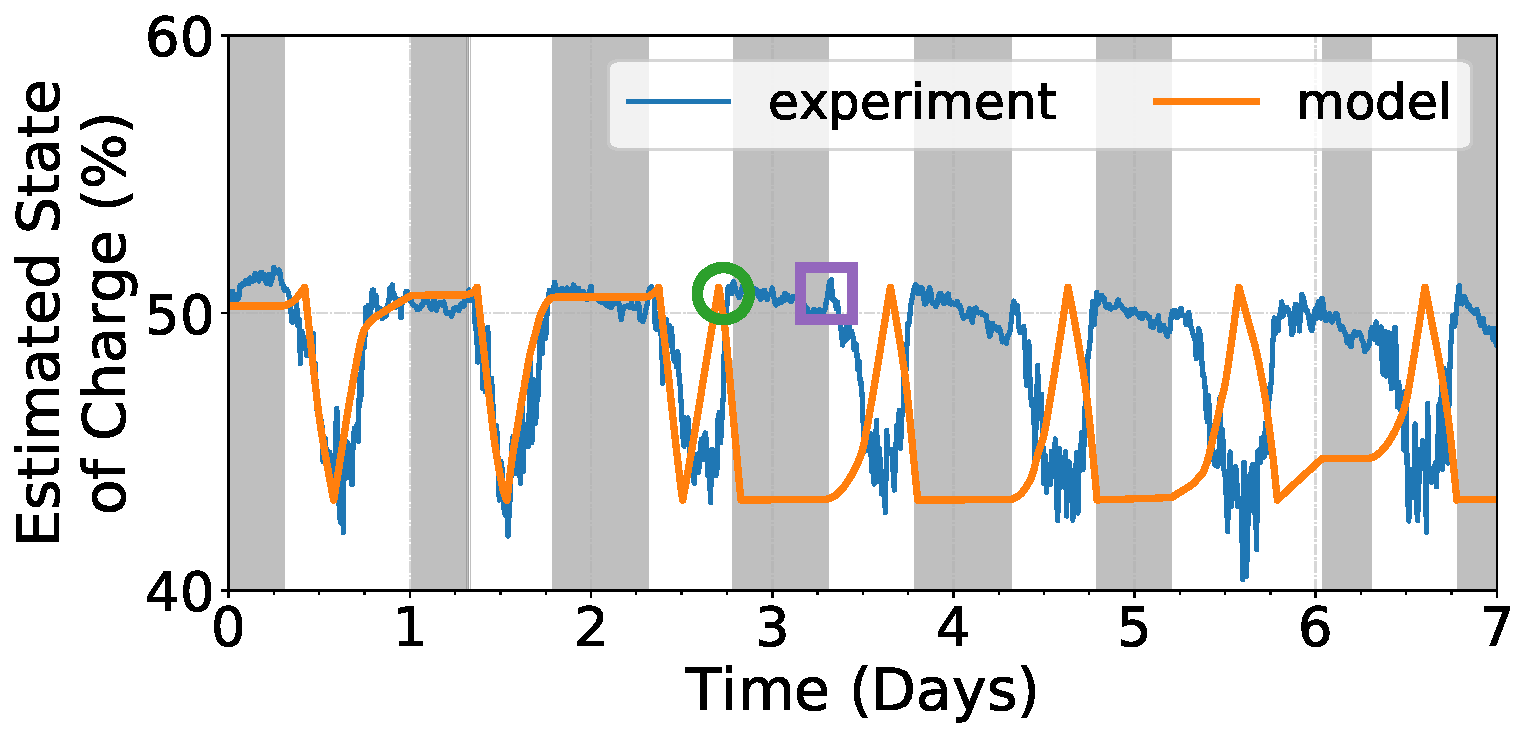
\includegraphics[width=\columnwidth]{figs/capacity/experiment_soc/exp_vs_sim_soc}
    \label{fig:eval:soc}
    \caption{The estimated state of charge of a week of a workload compared to our model's estimation.
    We use three weeks of illuminance measurements %from a month-long deployment
    to estimate irradiance and model the number of packets transmitted by an
    batteryless node. Average daily error is 15\%, with a standard deviation
    of 17\%. (b) We model and measure a \name's state of charge while running a
    ``sense and send'' workload with a 1\,s period for a week, beginning at
    midnight on the first day. Charging hysteresis
    limits of the devices are set at 51\% and 43\%. 
    Shaded regions represent periods of low harvestable potential
    (<\,15\,\textmu W/cm\textsuperscript{2}),
    i.e. nighttime. 
    For the first two days, model predictions
    closely track the experimental measurements. Errors
    in hysteresis and irradiance estimation cause the model to reach its upper
    hysteresis sooner than the experiment does, annotated by the
    \textbf{\textcolor{fig-green}{green circle}}. In actuality, the device
    exits charging hysteresis at the peak marked with the
    \textbf{\textcolor{fig-purple}{purple square}}.
    More importantly, the
    frequency and length of periods spent using harvested
    energy collected in the secondary-cell (downward slopes) are identical.
    %For the batteryless node we see our model
    %underestimate the number of transmitted packets by 10-20\% except for the
    %first day which predicts significantly more packets.  We believe this error
    %is primarily due to a piecewise linear estimation of irradiance from our
    %collected illuminance data, when in reality the relationship is complex and
    %non-linear.  For (b) we estimate the state of charge of \name
    %based on the secondary
    %cell voltage. Differences between the estimated state of charge and the
    %modeled state of charge are primarily due to inflated voltage during
    %charging and voltage droop and bounce back when \name
    %draws current from the secondary-cell.
    %Even though estimated state of
    %charge is not accurate due to this voltage swing, it is clear that the
    %timing of charge and discharge aligns between the model and the
    %experimental data.
    }
\end{definefigure}

\begin{definefigure}{fig:evalcmp}
    \centering
    \includegraphics[width=\linewidth]{figs/capacity/experiment_sys_compare/exp_packets_recv}
    \caption{
      \normalfont
        Packets received over two days.
      This figure compares the availability of an
      batteryless design and \name. \name sends a packet every second and does
      so without fail, while the batteryless system is only able to send when
      light is available.
      %This results in periods at night where the
      %batteryless device does not harvest enough energy to sustain operation.
      }
\end{definefigure}

\begin{definefigure}{fig:impl:permamote_life}
    \centering
    \includegraphics[width=\linewidth]{figs/capacity/primary/sense_and_send_life_vs_sec_size_permamote.pdf}
    \caption{
        Lifetime estimation of the \name sense and send workload given different rechargeable buffer sizes and different primary cell sizes. This figure utilizes the low irradiance Setup A environment and the 30 second sense and send workload period.
      This is a different presentation of \cref{fig:capacity:primary} that identifies the rechargeable capacity of \name with a red vertical line.
      }
    
\end{definefigure}

\begin{definetable*}{tab:related}
  \begin{threeparttable}
  \centering
  \begin{tabularx}{\columnwidth}{@{\extracolsep{\fill}} l | c c| c c| r}
      \thead[l]{Platform} & \multicolumn{2}{c}{\thead{Successful Events\,(\%)}} & \multicolumn{2}{c}{\thead{Long-Running\\Time to Completion Ratio}} & \thead[r]{Lifetime\\(yrs)}\\
                              & Periodic     & Reactive                     & Average & 95th Percentile & \\
    \hline
    Telos \cite{polastre2005telos}                      & 100   & 100   & 1     & 1     & 8.55\\
    Hamilton \cite{kim2018system}                & 100   & 100   & 1     & 1     & 6.75\\
    BLEES \cite{adkins2015michigan}                     & 100   & 100   & 1     & 1     & 1.11\\
    Gecko \cite{yervaGrafting12}                 & 39.5  & 64.9  & 387   & 981   & $\infty$\,\tnote{g} \\
    Capybara~\cite{colinReconfigurable18}\,\tnote{a}    & 46.3  & 72.8  & 37.6  & 1     & $\infty$\,\tnote{g}\\
    Capybara~\cite{colinReconfigurable18}\,\tnote{b}    & 41.1  & 67.1  & 2730  & 8900 & $\infty$\,\tnote{g}\\
    Flicker \cite{hesterFlicker17}                      & 39.3  & 64.2  & 1307  & 5670 & $\infty$\,\tnote{g}\\
    EnHANTs \cite{margolies2015energy}                  & 79.4  & 96.0  & 1     & 1     & \textemdash\,\tnote{h}\\
    DoubleDip \cite{martin2012doubledip}                & 77.9  & 66.5  & 1     & 1     & \textemdash\,\tnote{h}\\
    \cite{raisigel2010autonomous}                       & 78.4  & 66.9  & 1     & 1     & \textemdash\,\tnote{h}\\
    \textbf{\name}\,\tnote{c}                           & 81.2  & 98.3  & 1     & 1     & \textemdash\,\tnote{i}\\
    \textbf{\name}\,\tnote{d}                           & 100   & 100   & 1     & 1     &  35.8\\
    \textbf{\name}\,\tnote{e}                           & 100   & 100   & 1     & 1     &  30.2\\
    \textbf{\name}\,\tnote{f}                           & 100   & 100   & 1     & 1     &  6.27\\
  \end{tabularx}
    \begin{tablenotes}[para]
      \item[a] With capacitors: 400\,\ssi{\micro\farad} ceramic + 330\,\ssi{\micro\farad} tantalum + 67.5\,mF supercapacitor.
      \item[b] With capacitors: 300\,\ssi{\micro\farad} ceramic + 1100\,\ssi{\micro\farad} tantalum + 7.5\,mF supercapacitor.
      \item[c] No primary-cell.
      \item[d] AA primary-cells like Telos.
      \item[e] CR123A primary-cell like Hamilton.
      \item[f] CR2032 like BLEES.
      \item[g] Lifetimes are theoretically infinite for capacitor-based systems.
      \item[h] Not enough information to predict cycling failure time for theses systems.
      \item[i] Expect cycling degradation in 20-50 years, but do not attempt to estimate.
    \end{tablenotes}
  \end{threeparttable}
  \caption{
  \normalfont
      Simulated performance of energy-harvesting systems performing the same workloads.
    For each  platform considered, we model the performance of its energy storage
    architecture. Periodic workload and lifetime estimates are based on a 10\,s
    period, and the reactive workload is scaled to
    generate a maximum of 2000 events per hour (3.4\,s average daily period). 
    \name is the only energy harvesting platform that can provide 100\% availability, while also offering a lifetime of more than triple that of similar battery-only platforms.
    }
\end{definetable*}

\section{Image-based Occupancy Detection}
Besides the utilization of LED lighting and daylighting, another way to increase lighting efficiency in buildings is to automate lighting power states based on human occupancy.
Human occupancy is also a useful metric for regulating building heating and cooling.
The presence and number of people in a space directly effects the amount of heating, ventilation, and air conditioning (HVAC) a building must perform to maintain a temperature set point~\cite{wei2020deep}.
Compared to lighting, building HVAC is much more energy intensive, with cooling consisting of 10\% of the total U.S. electricity consumption in 2021~\cite{aeo2022}. 
Occupancy is measured in lighting control systems, however they often rely on a binary indication of occupancy based on simple ultrasonic or PIR motion detection~\cite{levitonDecora}.
This technique can not quantify the occupancy of a space, and it is prone to false positives and negatives.
Non-human objects that move through a space can trigger an ultrasonic sensor, while any rapid changes in surface temperatures can result in false positives for a PIR sensor.
When a person is not moving sufficiently, both ultrasonic and PIR sensors may sense a false negative.
Instead of, or in addition to these binary occupancy measurements, image sensing can be used to more accurately capture the occupancy, including person count, of a space.
Image inference, including classification and object detection, has been one of the most active areas of modern computer science and machine learning research. 
However, due to the cost and difficulty of deploying wired cameras, long-lived applications based on continuous image sensing has traditionally been untenable.
This is especially true for indoor building-centric applications, where camera density must be higher for sufficient coverage and lifetime must be sufficient to avoid frequent maintenance.

\subsection{Related Work}
Indoor wireless camera sensors have been heavily researched and commercialized over the past fifteen years, but due to the technology available at the time, as well as incompatibilities between design decisions and longevity, these platforms are typically limited to lifetimes of at most weeks to months~\cite{rowe2007firefly,rahimi2005cyclops,blinkindoor,wyzeoutdoor,josephson2019wireless}. 
Deployment of these platforms beyond small or temporary installations remain a challenge due to the cost of frequent battery replacement.
%With the confluence of new and improved COTS technology, like low power processors, radios, and image sensors, it is worth revisiting the design of wireless camera sensors. 

Modern image sensing platforms have taken advantage of technology improvements, as well as employed new techniques to reduce transmit power and increase (or abolish) lifetime. WISPCam~\cite{naderiparizi2015wispcam}, is a battery-free camera that utilizes RFID for power and backscatter communication. It can capture an image every 15 minutes when an RFID reader is 5 meters away. BackCam~\cite{josephson2019wireless} is  another camera platform that utilizes backscatter for communication, but over commodity WiFi. BackCam can stream video at 4 frames per second for a lifetime of 32 days. Similar to WISPCam, BackCam also requires a nearby wall-powered transmitter to generate excitation packets for backscatter communication. Camaroptera~\cite{nardello2019camaroptera} is another batteryless platform, focused on wide-area image sensing. 
The platform uses a long-range LoRa radio and harvests energy from solar panels. It performs local inference to detect people within captured photos and can achieve an end-to-end latency of less than 20 seconds in well-lit outdoor environments. Commercial platforms like the Blink Indoor wireless security camera~\cite{blinkindoor} and the Wyze outdoor camera~\cite{wyzeoutdoor} utilize low power motion detection to minimize energy usage. The Blink Indoor claims a 2 year lifetime consisting of 40000 seconds of recording 720p video on two AA batteries. Wyze estimates a lifetime of three to six months on its internal 5.2\,Ah battery if capturing 10 to 20 video clips per day.

While these modern platforms push the envelop for video streaming or batteryless imaging, they have drawbacks that limit their deployability in indoor spaces. Backscatter-based systems require a nearby carrier transmitter to communicate. Even with a dedicated, nearby transmitter, WISPCam can only periodically capture images every 15 minutes. Camaroptera is designed for outdoor use, and it is unclear if it can capture and send images indoors, especially as its energy harvesting system requires 197\,\uW when idle. 
The Blink camera lasts two years if it is placed in locations infrequently occupied by people. Placing the camera in a kitchen that sees an average 26\% occupancy on weekdays leads to a lifetime of only 1.78 days \cite{josephson2019wireless}. The Wyze camera faces a similar fate if placed in a frequently occupied area.

Image sensing platforms developed by industry and in research exhibit the same design disconnect that we noted in \cref{chap:background}. Commercial image sensing systems largely utilize batteries and avoid energy harvesting, while modern research systems are largely energy harvesting and batteryless.
These two different design result in a deceptive choice between reliable operation with a preallocated energy source but a limited lifetime, or an unlimited but unreliable lifetime with batteryless energy harvesting.
Neither option is satisfactory for many applications, including our indoor human occupancy detection example application that simultaneously demands a long sensor lifetime and high availability.

\subsection{The Performance of a Batteryless Image Sensor}
In this dissertation, we have argued that a batteryless approach is not appropriate for applications with QoS requirements. Designers of batteryless systems rarely evaluate their platforms and frameworks in regards to availability and reliability. However, utilizing the heuristics and simulation tools we have developed in \cref{chap:intuition,chap:capacity}, we can estimate the performance of these systems and identify alternate design decisions that may result in a more performant image sensing system.

In this section, we consider the design and performance of Camaroptera, a batteryless image sensor
~\cite{nardello2019camaroptera,desai2022camaroptera}.
We capture the design details of Camaroptera and use them to simulate the system and examine its performance.
Camaroptera is designed as a primarily outdoor system, and utilizes LoRa for communication and image backhaul.
It performs local inference to detect people in captured frames. A positive detection results in transmitting an image, and if no person is detected, it discards the captured image to preserve energy. 
It harvests solar energy with four small high-efficiency (20\%) monocrystaline solar panels (6.2\ssi{\centi\meter\squared} total area).  Camaroptera stores harvested energy in a 33\ssi{\milli\farad} supercapacitor.
Camaroptera, like many batteryless systems, operates opportunistically. 
Whenever its capacitor is charged sufficiently, it turns on and  performs its workload. 
Camaroptera's workload consists of capturing an image, performing some computations and inference on this image, compressing the image, and finally transmitting the packetized image. 
Camaroptera's energy storage is sized to support the most energy intensive operation in its workload: transmitting a single LoRa packet.
A single packet can not fit an entire compressed image, so Camaroptera relies on multiple power cycles to send between seven and eight packets to transmit an entire image.
All combined, a single image capture and transmission requires 781\ssi{\milli\joule}\footnote{Capture energy: 3.06 (capture) + 0.253 (difference) + 66 (inference) + 40 (JPEG) + 96$\times$7 (transmission) = 781\ssi{\milli\joule}~\cite{desai2022camaroptera}}.
When idle, Camaroptera's power subsystem consumes 197\ssi{\micro\watt}.
With this information, along with operation timing provided by the authors~\cite{desai2022camaroptera}, we are able to complete a simulation configuration like \cref{tab:capacity:parameters} for Camaroptera's hardware design and workload.

For energy income, we synthesize an outdoor irradiance trace based on the EnHANTs Setup D trace. 
The authors evaluated Camaroptera from 5--95\ssi{\kilo\lux}, which roughly corresponds to 4--77\ssi[per-mode=symbol]{\milli\watt\per\centi\meter\squared} for natural light\footnote{For natural sunlight: 1\ssi[per-mode=symbol]{\watt\per\meter\squared} $\approx$ 
122\ssi{\lux}~\cite{michael2020conversion}}.
We scale the mean of the synthesized outdoor trace to represent 10 and 50\ssi[per-mode=symbol]{\milli\watt\per\centi\meter\squared} for an estimate of outdoor irradiance on the same scale.
The simulation results of Camaroptera's average packet distribution under these two harvesting conditions are summarized by \cref{fig:impl:camaroptera_pkt}.
With either income, Camaroptera is able to maintain high image capture and transmit rates when light is available. 
However, as expected of a batteryless system, when light is unavailable, Camaroptera is unable to capture and send many images.
Since Camaroptera performs its workload in response to its energy storage state, it can not maintain a periodic schedule or reliably react and detect the presence of people.

\placefigure{fig:impl:camaroptera_pkt}

This limitation is primarily due to the energy capacity available to the platform. The available energy in an outdoor setting is essentially limitless to a low power embedded system like Camaroptera. 
For the two simulations we consider, our simulated Camaroptera with its capacitor energy buffer is only able to capture 48\% and 21\% of the available energy for the 10 and 50\ssi[per-mode=symbol]{\milli\watt\per\centi\meter\squared} traces, respectively. 
Due to its designed energy capacity, Camaroptera is simultaneously limited in the amount of energy it can capture and the amount of instantaneous energy available to it at any given time.
Given the design heuristics developed in \cref{chap:intuition}, we can determine an estimate for Camaroptera's average income and average workload power if we assume a fixed sensing period instead of the opportunistic operation of the actual platform.
From these averages and using the capacity sizing heuristics from \cref{sec:intuition:capacity}, we can determine an estimate for the minimum sufficient capacity to sustain this workload given our synthesized incomes.
As mentioned earlier, each Camaroptera activation requires 781\ssi{\milli\joule} over 40 seconds, assuming all images go through the entire inference pipeline. The platform's idle power is 197\ssi{\micro\watt}.
While the platform is capable of transmitting an image every 45 seconds to two minutes depending on lighting conditions, we assume a relaxed periodic rate of capturing and transmitting an image every five minutes.
This results in a 2.8\ssi{\milli\watt} average workload power\footnote{~$\frac{781\si{\milli\joule} + (197\ssi{\micro\watt} \times (300 - 40)\si{\second})}{300\si{\second}} = 2.77\si{\milli\watt}$}.

\placefigure{fig:impl:cam_sweep}
From this example workload and Camaroptera's income, we can use the huristics developed in \cref{chap:intuition} to determine the proper capacity sizing for the platform.
With Camaroptera's designed solar panel size, maximum power point voltage, and efficiency, 
it can expect between 12.3 and 61.6\ssi{\milli\watt} average income power from our two synthesized traces.
On average, this theoretical energy income should be more than sufficient to power this periodic sense and send workload, assuming the platform has enough capacity to capture it.
The lower end of this income corresponds to an income margin of over 300\%. 
Considering the sizing factor for income resembling the distribution of Setup D, determined in \cref{sec:intuition:margin}, we should expect a minimum sufficient capacity that is \num{1.4E3} times Camaroptera's workload power. 
This corresponds to an energy capacity of 3920\ssi{\milli\Wh}. 
The 33\ssi{\milli\farad} supercapacitor on Camaroptera only provides 41\ssi{\micro\Wh}. This capacity represents five orders of magnitude less than the minimum sufficient energy capacity predicted by our heuristic.
To further explore the impact of capacity sizing for Camaroptera, we simulate the platform with a sweep of different amounts of rechargeable capacity. 
We change our simulated Camaroptera's workload behavior from an opportunistic strategy to the periodic schedule discussed above.
We sweep capacity from the size of Camaroptera's original energy capacity to the amount predicted by our sizing heuristic.
The results of the simulated platform performance versus capacity are presented in \cref{fig:impl:cam_sweep}.
For each successive simulation that increases energy capacity, the periodic Camaroptera workload is able to achieve higher availability.
With an energy capacity above 100\ssi{\milli\watt\hour}, simulations with the 50\ssi[per-mode=symbol]{\milli\watt\per\centi\meter\squared} income are able to achieve near 100\% availability, while it requires at least 1000\ssi{\milli\watt\hour} for the 10\ssi[per-mode=symbol]{\milli\watt\per\centi\meter\squared} simulations to achieve similar levels of availability. 
Both of these simulation results suggest less energy capacity is required than the previously estimated 3920\ssi{\milli\Wh}.
This is for the same reason as explained in \cref{sec:impl:permamote}: the simulation begins with a partially charged energy buffer to mimic how a real system would be deployed while the heuristic analysis assumes starting from empty.
Thus, the heuristic provides a more conservative estimate that is more likely to result in energy neutral operation over longer periods of time.

Camaroptera was implemented with an energy capacity that was sized to support its most energy intensive task. This arbitrary design decision results in a minimally feasible design that is fails to fully capture and utilize the 
%more than sufficient 
available harvestable energy.
With significantly more energy capacity, Camaroptera would be able to capture more energy, persist through periods of no harvesting potential, and provide significantly higher availability. 
Based on the capacity requirements determined by this analysis, Camaroptera could be redesigned with a medium-sized rechargeable battery, on the order of 1000\ssi{\Ah}, to achieve the higher performance estimated in \cref{fig:impl:cam_sweep}.

\begin{definefigure}{fig:impl:camaroptera_pkt}
    \centering
    \includegraphics[width=\linewidth]{figs/chap6/camaroptera_performance.pdf}
    \caption{
        The distribution of simulated Camaroptera transmitted image packets per hour in a day. 
        The distribution represents an average over the length of two synthesized outdoor traces (10 and 50\ssi[per-mode=symbol]{\milli\watt\per\centi\meter\squared}) based on the EnHANTs Setup D trace. 
        Camaroptera operation is limited to times when daylight is available, regardless of the scale of average input power. The average number of packets is significantly lower between 6PM and 6AM.
     }
\end{definefigure}

\begin{definefigure}{fig:impl:cam_sweep}
    \centering
    \includegraphics[width=\linewidth]{figs/chap6/camaroptera_simulation.pdf}
    \caption{
        The availability of Camaroptera running a five minute sense and send workload, as energy capacity is increased from that offered by its original 33\ssi{\milli\farad} supercapacitor to the minimum sufficient capacity estimated by the heuristics developed in \cref{sec:intuition:capacity}.
        Capacity must be increased by five orders of magnitude in order to achieve near 100\% availability.
     }
\end{definefigure}

\subsection{The Design of an Indoor Wireless Image Sensor}
Due to Camaroptera's relatively high active and idle power requirements, it is unsuitable for use in many indoor environments. 
Designing an image sensor for indoor use will require different design decisions to achieve lower power operation.
An indoor sensor does not need to depend on higher power wide-area communications like LoRa. Instead, with  modest infrastructure investment, an indoor platform can rely on low power personal- or local-area networks.
Besides data transmission efficiency, power efficiency can be improved through the use of a more efficient and capable processor.
Idle power requirements can be reduced through the elimination of Camaroptera's hysteresis circuitry, and instead utilizing simple power gating to reduce component quiescent power. 
Using the heuristics and simulation tools developed, we can also identify the appropriate size of our energy harvesting, buffer capacity, and non-rechargeable storage to maximize energy available to our application. 
The next few sections expand on these design changes for indoor image sensor we name \namec.

\subsubsection{Indoor Wireless}
We design \namec to be untethered from wired communication and power. There are several options we consider for \namec's networking, including WiFi, and personal area networks like BLE and 802.15.4. WiFi is attractive as it supports high bandwidth, which would be appropriate for transmitting large data like images. However, many low power WiFi SoCs like the ESP32 have significant idle and startup power requirements~\cite{esp32}. 
If included on \namec, a WiFi radio or SoC must act as an external, power-gated component to reduce idle current. 
This complicates system design, and it is unclear if WiFi start up cost is worth the bandwidth advantage. 
Instead, we focus on technologies like BLE and networks built on top of 802.15.4. 
These networks are specifically designed to cater to devices that spend the majority of their lifetimes in an ultra low power sleep state. 
We trade off bandwidth and the time to send images for a simpler design and lower overall power.
 
%We utilize 6LoWPAN to enable a modern, IP-enabled design that allows direct end-to-end communication between sensors and the desired endpoint. We design a low power end-to-end image transfer architecture that makes images captured by \name{} easily accessible in high level languages and machine learning frameworks.
%To reduce the energy and time required to send images, \name{} compresses each image captured before transmission. 
%The use of IPv6 enables \name{} devices to directly send images to endpoints without any custom application layers. Received images can then be used for inference or published on a data stream.

\subsubsection{Processor Selection}
Processing and manipulating images requires significant computing and memory resources when compared to sensor data with lesser dimensionality, like periodic illuminance and color sensor data that is collected by \name.
Camaroptera's 16--bit, 16\ssi{\mega\hertz} processor requires 25 seconds of constant computation to compress a 160$\times$120 JPEG image with floating point emulation, and seven seconds to compress the same image with a fixed point algorithm.
This represents a significant amount of time for a low power device to be active and continuously computing.
The Camaroptera design is severely limited in digital signal processing by its processor selection. 
For \namec, we consider more capable, faster, processors with a 32--bit path and floating point support. 

\subsubsection{Power Supply}
Like \name, to support fully wireless operation for a long lifetime, \namec optimizes energy harvesting and storage through the use of rechargeable and non-rechargeable batteries.
As we have explored previously in our analysis of Camaroptera, vision applications require significant energy to capture images, process them, and transmit them. 
We size \namec's battery in the same manner as \name, utilizing the heuristics and simulation tool from \cref{chap:intuition,chap:capacity} to determine a sufficient capacity.
To determine this, we take benchmarks of capturing and transmitting images over an 802.15.4 network, and utilize these benchmarks to estimate an average power.
We utilize the same indoor irradiance traces that we considered previously.

Indoor energy harvesting is inconsistent and variable, and \namec will operate close to the edge of harvestable power that is reasonably available in many indoor environments.
To augment harvested energy, we include a backup nonrechargable battery on \namec. A backup battery allows continuous operation regardless of energy harvesting conditions. 
It safeguards the system from the volatile nature of energy harvesting, at the cost of a finite, but very long, lifetime.
%For intermittent sensors, this unreliability means the system can lose power at any moment, and any volatile state will be lost. These systems deal with this unreliablity in a number of ways, including techniques like checkpointing~\cite{luciaIntermittent17} and federated or reconfigurable capacitor storage~\cite{hester2017flicker,colin2018reconfigurable}.
%Intermittent capacitor-based systems utilize techniques like checkpointing \cite{luciaIntermittent17}, where the processor saves execution state before running out of power allow these platforms to continue to make forward progress on tasks.  
%However, as their operation is inherently tied on the availability of harvestable energy, they can not maintain any guarantees about reliability. 

\subsubsection{Other Considerations}
\namec includes additional sensors besides a camera to limit duty cycle and minimize idle power. A PIR sensor is used to sense motion, providing an ultra low power wake up mechanism for capturing images. Performing imaging on event detection instead of periodically can save considerable amounts of energy and extend lifetime. The platform also has a light sensor that can interrupt on large changes in light illuminance. This provides another wake up mechanism, allows \namec to detect when it is too dark to capture a useful image, and enables illuminance calibration for captured images. Both PIR and illuminance sensors require many orders of magnitude less energy than an image sensor to sense motion or illuminance.

To address the long-term relevancy of the platform, we also support an over-the-air update mechanism such that \namec can receive regular updates to improve energy management. Additionally, updates can be used to deploy new inference algorithms and models, as well as change image capture workload behavior. The platform can be configured to periodically take pictures, use the low power wake up mechanisms mentioned previously, or use some other software heuristic to only send interesting images.

\subsection{\namec Implementation}
\begin{definefigure}{fig:block}
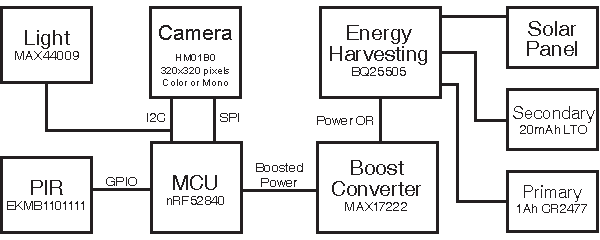
\includegraphics[width=\columnwidth]{figs/permacam/figs/block_diagram.pdf}
\caption{\name system block diagram.
The system is based on the Himax HM01B0 camera and the Nordic NRF52840 MCU. We include a light and PIR sensor to provide a low power wake up mechanism to drive image capture. A hierarchical energy harvesting system with a rechargeable and non-rechargeable battery are utilized to provide a long, reliable lifetime to the system.
}
\end{definefigure}

\begin{definefigure}{fig:arch}
\centering
\includegraphics[width=\columnwidth]{figs/permacam/figs/arch.pdf}
\caption{The \namec end-to-end image transfer architecture. \namec uses OpenThread, a 6LoWPAN network. This allows it to transmit images over the CoAP block protocol directly to any IP endpoint. We implement a CoAP server to receive and reassemble image, demosaic them, and publish them over an MQTT stream. This CoAP server can be local to the sensors if privacy is desired. User applications running on PCs or on servers can easily subscribe to incoming images.
}
\end{definefigure}

\begin{definetable}{tab:permacam:components}
    \begin{threeparttable}
        \centering
        \footnotesize
        \begin{tabularx}{\columnwidth}{@{\extracolsep{\fill}} l | l | c | c}
            Component                           & Function                     & Active Current          & Idle Current \\
            \hline
            Himax HM01B0                        & Image sensor                  & 2.0 mA                & 25.1\,\uA\,\tnote{a} \\
            \multirow{2}{*}{Nordic NRF52840}    & Processor                     & 52\,\uA/MHz           & 3.16\,\uA\,\tnote{b}  \\
                                                & Radio                         & 4.8\,mA @ 0\,dbm      & \textemdash\,\tnote{b}\\
            Ambiq AB1815-T3                     & Real time clock               & 55\,nA                & N/A\,\tnote{c}  \\
            Maxim MAX44009                      & Light sensor                  & 650\,nA               & N/A\,\tnote{c}  \\
            Panasonic EKMB11011                 & PIR Occupancy                 & 100\,\uA              & 1\,uA  \\
        \end{tabularx}
    \end{threeparttable}
    \begin{tablenotes}[para]
    \scriptsize
    \item[a] Power gated when not in use.\\
    \item[b] Sleep current for both processor and radio, full RAM retention, wake on low freq. timer.\\
    \item[c] No shutdown or idle mode.
    \end{tablenotes}
    \vspace*{1mm}
    \caption{
    \normalfont
    The components used in \namec, many of which are shared by \name. They represent some of the lowest power options currently available. Due to the extremely low idle power of all included components, \namec is able to sleep at 4.4\uA. 
    }
\end{definetable}

\begin{definefigure}{fig:demosaic}
\centering
\begin{subfigure}{0.49\columnwidth}
\includegraphics[width=\columnwidth]{figs/permacam/mosaic.jpeg}
\end{subfigure}
%
\begin{subfigure}{0.49\columnwidth}
\includegraphics[width=\columnwidth]{figs/permacam/demosaic.jpeg}
\end{subfigure}
\caption{\normalfont{An image from \namec, displayed as a mosaiced image (left) and demosaiced (right).}}
\end{definefigure}

\begin{definetable}{tab:measurements}
\centering
\begin{tabular}{l S[table-format=1.3] S[table-format=2.2]}
{Operation} & {Latency (s)} & {Energy (mJ)} \\
\hline
{Image Capture}           & 1.10  & 4.96\\
{JPEG Compression (Q=90)} & 0.203 & 1.71\\
{Image Transmission}      & 6.67  & 73.8\\
\hline
Total                   & 7.97 & 80.5
\end{tabular}
\caption {
    Latency and energy measurements for key operations on \namec{}, including image capture, compression, and image transmission. Measurements are averaged over 20 images. %An image capture actually consists of multiple frames to calibrate the exposure. We configure \name to wait four frames before capturing an image.
}
\end{definetable}

\begin{definefigure}{fig:impl:permacam_sweep}
\centering
    \includegraphics[width=\columnwidth]{figs/chap6/permacam_simulation.pdf}
    \caption{
        Lifetime estimates from \namec simulations with various rechargeable and non-rechargeable energy capacity. The addition of energy harvesting results in capturing more than double the energy provided by a non-rechargeable cell alone. The addition of a CR2477 results in over five years of lifetime for \namec.
    }
\end{definefigure}

In this section, we explore the implementation of \namec{}, including component selection, techniques to enable a low power camera interface, and architectural details about the energy harvesting and storage architecture

\placefigure{fig:block}

We implement the design of \namec{} in an \textbf{open source}
hardware\footnote{\url{https://github.com/lab11/permamote/tree/master/hardware/permacam/rev_a}}
and software\footnote{\url{https://github.com/lab11/permamote/tree/master/software/apps/permacam/camera_coap}}
implementation. The platform is built around the Himax HM01B0 ultra low power camera \cite{hm01b0}. This camera has also enabled other platforms like BackCam \cite{josephson2019wireless} and Camaroptera \cite{nardello2019camaroptera}. The Himax camera is available in two different versions: monochrome and color. 
We use the color version of the sensor to ensure the ability to capture color information of images, but the two versions are pin compatible and can be interchanged. The other key component of the design is the SoC processor. 
For a processor, we select the Nordic nRF52840 Cortex-M4F SoC as it is one of the most power efficient processors available, includes a Floating Point Unit (FPU), and is relatively fast compared to other low power microcontrollers at 64\,MHz. 
An FPU allows the platform to perform floating point dependent tasks like image compression. 
It has a multiprotocol BLE/802.15.4 radio that is well supported by OpenThread, an open source implementation of the Thread 6LoWPAN mesh network protocol~\hl{todo cite}. 
It features comparatively large amounts of flash (1\ssi{\mega\byte}) and SRAM (256\ssi{\mega\byte}), which is enough to capture images and perform some local processing. 
We include an ultra-low power real time clock (RTC) to provide accurate image timestamps. 
The platform also features an ultra low power PIR sensor and illuminance sensor to provide a low power wakeup mechanism and illuminance calibration for captured images. 
A block diagram of the major system components is displayed in \cref{fig:block}. 
Characteristics of the sensors and the MCU are summarized in \cref{tab:permacam:components}. 
In the next few sections we describe \namec{}'s implementation, including the MCU to camera interface, energy harvesting architecture, image compression methods, the end-to-end image transmission architecture, and an implementation of onboard person classification.


\subsubsection{Camera Interface}
The majority of image sensors do not support normal sensor interfaces like I2C or SPI to transfer data. Instead they rely on high frequency ($\geq$8\,MHz) serial or parallel data busses. This is because images are many kilobytes or megabytes in size, and data transfer must be at a high frequency or parallel to transfer multiple frames per second. The majority of embedded processors, the nRF52840 included, are not designed to interface with parallel camera busses. Traditionally, platforms have used intermediate hardware like dedicated processors, CPLDs or FPGAs to interface with image sensors and buffer frames \cite{rowe2007firefly,rahimi2005cyclops}. The Himax HM01B0 has two interfaces, an I2C command interface and a serial, 4x, or 8x data interface.
The Himax HM01B0 requires an input master clock (MCLK) of 3-36\,MHz to drive internal sensor timings and outputs a pixel clock (PCLKO), frame valid (FVLD), and line valid (LVLD) signals \cite{hm01b0}. It can be configured to capture full frame (320x320), QVGA (320x240), and if the mono version of the sensor, downscaled QQVGA (160x120) resolution images. In \namec{} we capture full frame images and use the color version of the sensor. 
This version produces color filter array (CFA) images. 
A CFA is an alternating "mosaic" of green-blue-green and red-green-red rows of pixels~\cite{bayer1976color}. 
Each pixel corresponds to a single color, and through post-processing known as "demosaicing", a three channel RGB image is generated from the single channel representation. 
An example of a mosaiced image and its demosaiced counterpart are displayed in \cref{fig:demosaic}.
\namec{}'s processor does not possess enough memory to locally demosaic an full image so any inference or transmission must be done with the mosaiced image. 
We power-gate the HM01B0 camera on \namec, allowing the system to completely power the camera off and enter the lowest possible power state.

\placefigure{tab:permacam:components}

Other systems that utilize the Himax HM01B0 camera including BackCam, Camaroptera, and the Sparkfun Edge have developed a bitbang protocol to emulate a parallel interface \cite{josephson2019wireless, nardello2019camaroptera, sparkfunedge}. This is possible because their processors support GPIO direct memory access (DMA). This allows the GPIO peripheral to directly write to memory, avoiding costly processor cycles to load GPIO state into registers and then write it to memory. This optimization allows a bitbang protocol on these platforms to operate faster than the HM01B0's minimum operating frequency. However, a bitbang protocol is undesirable because it requires the processor to be on during an image transfer, consuming additional energy. The nRF52840 does not support GPIO DMA. 
Because of this, developing a bitbang protocol that adheres to the required camera timing is infeasible. 
Instead, we note that the camera serial protocol closely resembles SPI, and the nRF52840 implements an 8\,MHz SPI peripheral with DMA support. 
The camera PCLKO signal is identical to SCLK, and can be gated by the LVLD signal. 
The LVLD signal from the camera indicates when a line of the image is being transmitted, and is analogous to a SPI chip select line. However, this line is active high, and most SPI implementations, including the hardware on the nRF52840, expect active low. Inserting a low latency inverter in between the LVLD output of the camera and the MCU allows the nRF52840 SPI peripheral to interface with the camera. 
This has the added benefit of reducing power required to read in images as the processor can sleep while the SPI peripheral directly writes images to memory.

\placefigure{fig:demosaic}

\subsubsection{Image Compression}
To reduce energy and time required to transmit images, we employ JPEG compression on images prior to transmission. We use the Moodstocks JPEC encoder, a simple and portable monochrome JPEG encoder written in C \cite{moodstocks}. JPEG compression, like most DSP algorithms, relies heavily on floating point arithmetic. Due to its integrated FPU, \namec{}'s processor is able to compress full resolution 320x320 images in 210\,ms.
This encoder is also used in Camaroptera \cite{nardello2019camaroptera}, although this platform is based on the MSP430, which lacks an FPU. It requires 25 s to compress an downsampled 160x120 image using floating point emulation, and 7s when JPEC is adapted to fixed point math. This fixed point adaptation also reduces image quality slightly. It is clear that a camera platform like \namec{} benefits greatly from the inclusion of a faster, more capable processor.
JPEG is not designed to compress mosaiced images. However, we find that monochrome compression with a high quality setting does not overly degrade image fidelity or color representation. We explore the effects of monochrome compression on \namec's captured images further in \cref{eval:compression}.

\placefigure{tab:measurements}

\subsubsection{Energy Harvesting and Storage}
The energy storage architecture for \namec{} is built around the TI BQ25505~\cite{bq25505} maximum power point tracking boost converter, like \name. 
The output of the BQ25505's power OR is boosted to the system voltage by a MAX17222 regulator to power all components under a single voltage domain.
We use a 10.9\ssi{\centi\meter\squared} amorpohous photovoltaic to charge a rechargeable LTO battery.
We size this LTO battery according to the capacity heuristic from \cref{sec:intuition:capacity}.
The \namec workload consists of an image capture, JPEG compression, and image transfer. These operations are benchmarked on the nRF52840 SoC and HM01B0 image sensor and summarized in \cref{tab:measurements}.
If we assume a periodic workload, capturing, compressing (at JPEG quality 90), and transmitting an image very ten minutes, \namec will require 148\ssi{\micro\watt} on average\footnote{~$\frac{80.5\ssi{\milli\joule} + 14.5\ssi{\micro\watt}\times(600-7.97)}{600}$}.
This workload for \namec is pushing the bound on the energy that is harvestable within an indoor environment. 
If we consider there is no harvesting margin, this suggests a minimum sufficient capacity on the order of \ssi{\milli\Wh}. 
This capacity corresponds closely to a 125\ssi{\milli\Ah} LTO battery with a nominal 2.4\ssi{\volt}, which is the closest size available for purchase.
We simulate \namec's workload under the conditions of EnHANTs Setups A and D, while sweeping capacity and considering several different sizes of backup batteries.
From the results, presented in \cref{fig:impl:permacam_sweep}, we can determine an appropriate backup battery size to achieve an acceptable lifetime.
We select a lithium 3\ssi{\volt}, 1\ssi{\Ah} CR2477 coin cell battery. This amount of backup energy results in a design that can persist more than five years while capturing an image every ten minutes.
\placefigure{fig:impl:permacam_sweep}


\subsubsection{End-to-end Image Pipeline}
To support transmitting full images, we implement a full application stack based on standard IP-based protocols. This end-to-end image architecture is depicted in \cref{fig:arch}.
We choose to use OpenThread, an open source implementation of the Thread network protocol for \namec devices. Thread is a 6LoWPAN mesh network, and allows packets to be sent end-to-end over a standard IP network. OpenThread also provides implementations of useful protocols like CoAP, SNTP, and DNS. 
CoAP is a lightweight restful protocol similar to HTTP, but over UDP \cite{shelby2014constrained}. 
On top of OpenThread's CoAP API, we implement the CoAP Block add-on feature. This allows us to fragment large data like an image across multiple CoAP payloads \cite{bormann2016block}. 
The choice to use CoAP block is a reluctant one however, and was based on the available implementations of reliable transfer protocols for low power networks.
\namec image transmission is a perfect application for TCP, although TCP is rarely implemented for low power networks. TCP has been shown to be provide a 40\% higher throughput compared to CoAP block over an OpenThread network~\cite{kumar2020performant} over an OpenThread network. However, TCP was not implemented in the version of OpenThread used during the implementation of \namec, limiting us to CoAP block.

\placefigure{fig:arch}

\namec captures an image, compresses it using JPEG, and transmits the image using a CoAP blockwise transfer. The CoAP block messages are sent to an endpoint that reassembles them, parses their contents, and publishes a JSON message over an MQTT broker. An application running on the endpoint listens for the transmitted mosaiced images, demosaics them, and republishes the color image for application use. High level applications wishing to interface with images captured by \namec devices simply must subscribe to the relevant device topics to receive images. From there, the images can be easily processed in frameworks like OpenCV, Tensorflow, or Pytorch~\cite{tensorflow2015-whitepaper, pytorch,itseez2015opencv}.

In addition to our data backhaul pipeline, we implement an independent update server. \namec devices arbitrarily poll the update server every 24 hours for a new application image. If a newer image exists, it downloads it over a CoAP blockwise transfer and applies it. This allows users to deploy new applications quickly across an entire deployment with minimal intervention.

\subsubsection{Local Image Classification}
In addition to transmitting images, we also demonstrate the ability of the platform to perform local inference.
While performing local object detection is not feasible with the memory and compute constraints of \namec,image classification (with a limited number of classes) is not. 
To explore the capabilities of machine learning inference on \namec,
we modify and train our own MobileNets v1 network to perform person classification. We then deploy it to \namec's processor using TensorFlow Lite for Microcontrollers. 

The parameter flexibility of MobileNets v1 allows us to reduce the size of the model so it can fit on a microcontroller. We reduce the size of the network by reducing the depth of each convolutional layer by 75\% ($\alpha$ = .25).  
%\hl{cut some of model details if space needed: }
The model consists of a regular convolution with batch normalization followed by multiple depthwise separable convolutions~\cite{howard2017mobilenets}. 
%The result of the convolutions is passed through an average pooling layer and a dense layer of 2 units, resulting in a person and no person score. A kernel size of 3 is throughout all convolutions.
There is insufficient memory to perform the forward pass on full sized 320x320 images, so images need to be downscaled. We configure this network for different input image dimensions including 48, 72, 96, and 120.
We train this model for 80 epochs on the Visual Wake Word dataset~\cite{chowdhery2019visual} to achieve a validation accuracy of 78\%, compared to a 90\% accuracy with an unmodified MobileNet. The model weights require 230\.kB after post-training quantization and achieve an accuracy of 76\% for input images of size 120x120 when using TensorFlow in Python. We deploy this model on \namec and evaluate its performance in \cref{eval:localinf}.

\subsection{\namec Evaluation}
\hl{TODO: need to go through this section and edit + fix figures}



\begin{definefigure}{fig:compression}
\captionsetup[subfigure]{labelformat=empty}
\centering
\begin{subfigure}{0.4\columnwidth}
\includegraphics[width=\linewidth]{figs/permacam/30.jpeg}
\vspace{-1.5\baselineskip}
\caption{30}
\label{fig:30}
\end{subfigure}
%
\begin{subfigure}{0.4\columnwidth}
\includegraphics[width=\linewidth]{figs/permacam/70.jpeg}
\vspace{-1.5\baselineskip}
\caption{70}
\label{fig:70}
\end{subfigure}
\par\medskip
\begin{subfigure}{0.4\columnwidth}
\includegraphics[width=\linewidth]{figs/permacam/93.jpeg}
\vspace{-1.5\baselineskip}
\caption{93}
\label{fig:93}
\end{subfigure}
%
\begin{subfigure}{0.4\columnwidth}
\includegraphics[width=\linewidth]{figs/permacam/raw.jpeg}
\vspace{-1.5\baselineskip}
\caption{raw}
\label{fig:raw}
\end{subfigure}
\caption{An image compressed with different quality factors. \normalfont{In this scene, we set smart lights to bright, intense colors to elucidate the effects of compression on color representation. Compression is performed on the mosaiced version of the image, which after transmission is demosaiced into the color representations displayed. Due to this, an image compressed with a low quality factor loses significant color information compared to the raw image. Luckily, high quality factors produce a near-indistinguishable representation of the raw image. We explore a more quantitative view of image similarity in \cref{fig:ssim}.}}
\end{definefigure}

\begin{definefigure}{fig:size-time-energy}
    \centering
    \includegraphics[width=\columnwidth]{figs/permacam/permacam_processing/size_time_energy.pdf}
    \caption{Effects of JPEG compression on image size, time to send, and energy to send.
        \normalfont{
            Compression provides exponential decrease in image size, which directly relates to decreases in the time and energy required to send images. Using a low quality factor results in images that are 8.2\% the size of the original raw image. The amount of time and energy required to send images exhibit more variance than image size. This is the result of occasional packet loss and backoff during image transmission. Larger images require more packets and thus exhibit a higher probability of this occurring.
        }}
\end{definefigure}

\begin{definefigure}{fig:ssim}
    \centering
    \includegraphics[width=\columnwidth]{figs/permacam/figs/jpeg_ssim.pdf}
    \caption{\normalfont{The image structural similarity index (SSIM) of images compressed at various JPEG quality factors.
        A higher SSIM indicates that an image is a closer representation to the original raw image.
        While a low quality factor results in smaller compressed images, it results in a significant loss in image structural similarity. Quality factors 90 and 93 provide a >90 SSIM, suggesting that they are near identical representations of the original image.
    }}
\end{definefigure}

\begin{definefigure*}{fig:lifetime}
\centering
\begin{subfigure}{0.445\textwidth}
\includegraphics[width=\linewidth]{figs/permacam/figs/lifetime_periodic.pdf}
\label{fig:lifetime_periodic}
\vspace{-1.5\baselineskip}
\caption{Periodic}
\end{subfigure}
%
\begin{subfigure}{0.545\textwidth}
\includegraphics[width=\linewidth]{figs/permacam/figs/lifetime_event_60.pdf}
\label{fig:lifetime_event}
\vspace{-1.5\baselineskip}
\caption{Reactive}
\end{subfigure}
\vspace{-1\baselineskip}
\caption{\normalfont{
    Estimated lifetime from a numerical model. Two workloads are simulated: periodic and reactive. A periodic workload takes a picture at a fixed interval, while the reactive workload models motion events captured by a PIR sensor. We vary the quality factor of images sent, which has a direct impact on the lifetime of the workloads. Each colored line represents a different period of the periodic workload, or the duration of the back off after an event for the reactive workload. As expected, the reactive workload results in a longer lifetime as it captures and transmits fewer images in times of less activity like nighttime. For both workloads, \name is able to transmit images compressed at quality 90 and still achieve a one to five year lifetime based on period or back off duration.
}}
\end{definefigure*}

\begin{definefigure}{fig:multiple}
    \centering
    \includegraphics[width=\columnwidth]{figs/permacam/figs/multiple_cameras.pdf}
    \vspace{-2\baselineskip}
    \caption{\normalfont{An image's time to send as number of \namecs on the network increases. All sensors are within one meter radius of each other, and configured to capture and transmit images on motion events to generate the worst case collision condition. Images are compressed with quality 90.
    }}
\end{definefigure}

\begin{definefigure}{fig:map}
    \centering
    \includegraphics[width=\columnwidth]{figs/permacam/figs/jpeg_mAP.pdf}
    \vspace{-2\baselineskip}
    \caption{\normalfont{Mean Average Precision (mAP) of YOLOv3 person detection on compressed images compared to original raw versions. An IoU of 0.5 is used. Based on the qualitative and quantitative results of image similarity from \cref{fig:compression} and \cref{fig:ssim} it is surprising that mAP degrades so quickly as the compression quality factor decreases. A quality factor of 90 or higher is necessary to achieve the near the same detection performance as a raw image}}
\end{definefigure}

\begin{definefigure}{fig:distance}
    \centering
    \includegraphics[width=\columnwidth]{figs/permacam/figs/distance_detection.pdf}
    \caption{\normalfont{
        Detection confidence as distance from camera to person is increased. Compared to a modern smartphone camera, the camera on \name can not compete due to limited resolution. However, images captured by \name still enable person detection at a distance of 15-20 meters. This distance is generally sufficient for most indoor spaces.
    }}
\end{definefigure}

\begin{definetable}{tab:local-inference}
\begin{tabularx}{\columnwidth}{l c c c c c}
Dimension (pixels) & Latency (s) & MOPs & Energy (mJ) & Memory (kB) & Accuracy (\%) \\
\hline
48 & 1.72 & 0.450 & 17.2 & 73.7 & 68.6 \\
72 & 2.71 & 1.01 & 27.0 & 91.0 & 69.2 \\
96 & 3.64 & 1.80 & 36.4 & 115. & 72.4 \\
120 & 5.10 & 2.81 & 50.9 & 146. & 74.7 \\
\end{tabularx}
\caption {
    Latency, millions of operations, energy, peak memory, and accuracy 
    of local person classification. Images must be downscaled from full resolution, as inference on a 320x320 image requires too much runtime memory. The quantized version of model weights are used to measure accuracy of the validation set. The highest accuracy achieved is only 74.7\%, and requires 5.1 seconds of continuous computation.
}
\end{definetable}

\begin{definetable}{tab:end-to-end}
\setlength\tymin{1cm}
\small
\begin{tabulary}{\columnwidth}{l c c c}
Compression\newline Quality & Size\newline(kB) & Latency\newline(s) & Energy\newline(mJ) \\
\hline
30  & 1.98 & 0.513 & 4.23\\
50  & 3.25 & 0.764 & 6.95\\
70  & 4.82 & 1.12 & 10.3\\
80  & 6.19 & 1.31 & 13.2\\
90  & 9.12 & 1.86 & 19.5\\
93  & 10.6 & 2.13 & 22.7\\
raw & 25.6 & 4.91 & 54.7\\
\end{tabulary}
\caption {\normalfont{Time and energy required to send 160x160 images end-to-end. Images are compressed with varying JPEG qualities. Sending compressed images requires less time and energy than performing person classification on lower resolution images.}}
\end{definetable}

\begin{definefigure}{fig:cycle-per-byte}
    \centering
    \includegraphics[width=\columnwidth]{figs/permacam/figs/cycles_per_byte.pdf}
    \caption{The required energy per byte of image data to run different algorithms on the processor used by \name{}.
        \normalfont{
            The slope of the solid line represents the energy per cycle of the processor. The dashed line represents the energy per byte of a compressed transmission of an image. Three algorithms are plotted here: JPEG compression with quality factor 90, our custom MobileNets v1 person classifier, YOLOv3-tiny object detection. We estimate the cycles and energy required of YOLOv3, as it requires more memory than available on our microcontroller.
        }}
\end{definefigure} 

We evaluate \name{} on our goals of deployability and capability through a number of experiments. We begin with an analysis of the effects of JPEG compression on image size, time to send, and energy. From this analysis, we use these measured metrics to estimate platform lifetime using different representative workloads. 
%We estimate platform lifetime using different configurations of workloads and image compression. 
We explore the capability of the platform by writing an object detection application on top of the \name{} end-to-end image transfer architecture. We evaluate the ability to detect objects in images captured by \name{} at varying qualities of compression and distance from the camera. We also implement local image inference in the form of person classification. We evaluate the performance of local classification, and compare it to image transmission.
%into the options for reducing energy spent transmitting images, including image compression and downsampling. We analyze the effects of these techniques have on resulting image quality. Based on the efficacy of image compression, we estimate lifetime using a simulation of \name{} to evaluate the longevity of the platform. We evaluate the capability of the platform by performing object detection tasks on the images that it captures. We measure the effects of design decisions on the accuracy of detections.  

\placefigure{fig:size-time-energy}

\subsubsection{Image Compression}
\label{eval:compression}
A raw, full frame image from \name{}'s camera is over 100\,kB in size. Sending these raw images requires a significant amount of time and energy. We employ JPEG compression to significantly reduce image size. This decrease in size comes at the cost of reduced image fidelity and color representation.

We use the Moodstocks JPEC encoder to compress captured images in JPEG format. JPEC is a monochrome JPEG encoder, and we have configured \name{} to use the color version of the HM01B0 image sensor. The images captured are a "mosaiced" color filter array, and performing monochrome JPEG compression on a mosaiced image reduces color representation in addition to image fidelity. JPEG can be configured with different quality factors from 1 to 100. A lower quality factor results in a less accurate representation and smaller compressed size. Image size relates linearly to the time and energy required to send images. 
We configure \name to capture images, compress them with 6 different JPEG quality factors and transmit them. We collect 60 images, each with 6 compressed versions, and analyze the effect of compression on image size, time to send, and energy to send.
The results are displayed in \cref{fig:size-time-energy}. 

\placefigure{fig:compression}

JPEG image compression allows an exponential decrease in image size with respect to the quality factor.
Compressing images at a high quality factor (JPEC's default 93) results in greater than a 2x reduction in image size, time to send, and energy required. There are diminishing gains after the knee of the curve at quality 90, but an image compressed with quality 30 is only 8\% the size of a raw image, on average. Image compression on mosaiced images from \name also does not appear to degrade the perceived quality of the image. We display four compressed and raw versions of the same image in \cref{fig:compression}. Qualitatively, and from a distance, these images appear nearly identical. However, closer inspection reveals artifacts and a significant loss in color fidelity with lower compression quality factors. Quality 93 and a raw image are nearly identical, while quality 30 is more obviously a lower quality compression. However, the important details in the image are preserved and still visible to the human eye.

\placefigure{fig:ssim}

To more quantitatively analyze the effects of compression on mosaiced images, we measure the Structural Similarity Index (SSIM)~\cite{wang2004image} of all 360 compressed images compared to their raw counterparts. SSIM is often used to measure the quality degradation of images due to compression or transmission. The results are summarized in \cref{fig:ssim}. A higher SSIM indicates that an image is a closer representation to the original raw image.
Even with a low quality factor of 30 or 50, the SSIM for images average above 0.75. With an image compressed with a high quality factor, the perceived similarity is above 0.9 and, as seen in \cref{fig:compression}, is almost indistinguishable from the raw image. These results suggest that using a quality factor of 90 or above on to compress images on \name is advantageous if we can afford the energy to send them.

\subsubsection{Camera Density}
While our numerical model can provide an accurate estimate of lifetime, it makes an important assumption. In our modelling, we assume that every image transfer requires the same amount of time and energy. The reality is that wireless environments can have interference, especially for low bandwidth networks like 802.15.4. The result of interference from other networks, devices, or other \namecs, means that packets will be dropped and retransmissions are necessary. This extends the length of image transmission and the increases required energy. 
We explore the scalability and effects of interference when multiple \namecs on the same network. We place all cameras within a meter radius of each other facing the same direction. The network consists of only one Thread router. Each \name is configured to simultaneously capture on a motion event to generate a worst-case collision scenario. Each camera is sending images compressed with quality factor 90.
%In real deployments, cameras are likely to be sparser and multiple Thread routers will be deployed for greater coverage. 
The \namecs are configured with a 2 minute backoff period after a motion event and camera capture. At the start of the experiment, a person walks into view of all the cameras, triggering them simultaneously. The person then remains in view of the cameras for half an hour. We vary the number of cameras active and measure the average time to send images over the duration of the experiment. The results are displayed in \cref{fig:multiple}.

\placefigure{fig:multiple}

We do not currently implement any application layer collision avoidance and we use the default 802.11.4 CSMA MAC protocol specified by Thread. Based on our naive implementation, having more than three \name sensors connected to a single router and on the same network leads to a dramatic increase in time to send images. Implementing an actual coordination protocol between \namecs would dramatically reduce collisions. Additionally, the use of  TCP instead of CoAP block would significantly reduce transmission latency and possible overlap.
%Luckily, during a CoAP backoff period after a missed packet, \name can return to a low power sleep mode, waiting for the back off to expire. 
Irregardless of these improvements, we expect most deployments of \name will be aware of the limitations and will only require one to two cameras per room.

%\subsubsection{Image downscaling}
%\hl{I only downscaled to 160x160 for comparison with local inference, is it worth it to mention here? Could just plot on same figures as above section}

\subsubsection{Object Detection Performance}
To illustrate the capability of the platform and end-to-end image transfer system, we evaluate the ability to perform object detection with \name. The images produced by \name are published over an MQTT stream, which feeds into a script that performs object detection using the pre-trained YOLOv3 network included in the Python ImageAI package \cite{ImageAI}. We do not wish to measure the accuracy and performance of the ImageAI YOLOv3 model, but instead isolate the ability to perform detections on images captured by \name's camera and the effects of different compression quality factors on detection performance.

\placefigure[t]{fig:map}

\subsubsection{Compressed detection accuracy}
While we measure the structural similarity of compressed images using SSIM, this does not directly relate to the performance of object detection on compressed images. To evaluate the effect of image compression on detection accuracy, we use the same 360 images used previously to measure the effects of JPEG compression. These images feature various representative objects of the classes supported by the YOLOv3 model in ImageAI. To quantify the effects of compression, we calculate the mean average precision (mAP) using an intersection overlap union (IOU) of 50\% of the detections compared to a raw image from \name. 
The metrics mAP and IoU=0.5 are both common metrics used to evaluate object detection algorithms. We refer readers unfamiliar with this metric to the Pascal VOC challenge paper~\cite{everingham2010pascal}.

%For a given detection, a bounding box is created. The IoU of this bounding box compared to ground truth is the ratio of the area of overlap to the area of the union between both bounding boxes. Currently, it is common to consider an IoU above 0.5 to be a true positive detection. Average precision (AP) is calculated by integrating the precision/recall curve of the detection results for a class. The mean AP (mAP) is the mean of all calculated AP
In \cref{fig:map}, we display the mAP for different JPEG quality factors. Surprisingly, images compressed with a lower quality factor perform much worse than their SSIM suggests. Images compressed with quality factor 30 and 50 achieve less than 40\% mAP, while factors above 90 achieve near identical detections to their raw counterparts.

\subsubsection{Limitations of resolution}
\name{}'s camera is limited in resolution and color representation compared to most image sensors in modern cameras and cell phones. For example, the Google Pixel 3 features a 12.2 megapixel image sensor, which offers two orders of magnitude more resolution than the HM01B0's 0.1 megapixel. A lower resolution places a limit on the size of objects and the distance at which they can be detected. If an object is only represented by a few pixels, there is unlikely to be enough information to successfully detect it. To evaluate the capability to perform object detection with images captured by \name{}, we compare detection accuracy to images captured by a modern cell phone camera. We successively capture images of a person at varying distances and measure the resultant detection accuracy, if any. The results are summarized in \cref{fig:distance}.

A person is successfully detected at a distance of 20 meters with images from \name{}, though confidence is only 16\%. Unsurprisingly, a person is easily detected at all distances tested with images taken by a Pixel 3. While images captured by \name{} can not compete with the resolution of those captured by cell phones, they are sufficient for detection at reasonable distances. Many indoor spaces do not have sight lines longer than 20 meters, and if they do, additional camera coverage can help mitigate the lack of resolution of a single camera. The ability to clearly depict objects in the distance is partially dependent on the lens configuration of a camera. During this experiment, \name{} was configured with a 200\textdegree\xspace wide angle lens. Better performance could be achieved with a lens with a narrower field of view and more magnification, at the cost of less coverage. We envision most applications will prioritize field of view to cover large areas instead of additional magnification.

\placefigure[t]{fig:distance}

\subsubsection{Local Inference}
\label{eval:localinf}
In addition to end-to-end image transmission, \name is also capable of local image inference. We implement and train a modified MobileNets v1 network using TensorFlow in Python~\cite{tensorflow2015-whitepaper} and the Visual Wake Word dataset~\cite{chowdhery2019visual}. Using TensorFlow Lite for Microcontrollers, we quantize and deploy the model to \name's processor.

We upload 20 images from the validation set to \name, and measure inference latency and energy. We measure inference accuracy across our validation set of 8059 images, using quantized weights in TensorFlow.
%perform inference on images and measure the latency, energy, and accuracy of predictions.  
The results are summarized in \cref{tab:local-inference}. Inference on the largest image dimension (120) requires just over 5 seconds of continuous computation and has a peak memory usage of 146\.kB to achieve a 75.1\% accuracy. This accuracy pales in comparison to what can be achieved with a full sized model running on more powerful hardware. Can local inference provide benefits to energy or latency to make up for its lackluster accuracy?

To answer this question, we also perform end-to-end image transmissions on \name to compare. Images are downsampled from 320x320 to 160x160 to compare with the downsampled images used for inference. They are 1.77x as large as the 120x120 images used for classification. Images are compressed using JPEG at varying qualities. We measure time and energy required to send images. The results of this experiment are summarized in \cref{tab:end-to-end}. Surprisingly, the average energy required to transmit images of this size is generally less than performing inference on them. 
%Generally, performing local person classification on images requires more time and energy than transmitting a compressed version of the image.
For example, we are able to transmit a 160x160 image compressed at quality 93 for under half the energy needed to perform inference on a smaller 120x120 image.
Considering the effort to deploy machine learning inference to a microcontroller, the marginal accuracy of shrunken models, and the demanding energy requirements, a simpler and more beneficial solution is to just transmit images to more capable endpoints.

\placefigure{tab:local-inference}

\subsection{To send or not to send}
This conclusion is unique to the design choices made for \name{} and its envisioned indoor application space. For example, outdoor applications have access to significantly more harvestable energy, but also have different, often higher power, options for wireless communication. Therefore, we seek to provide a generalizable guiding methodology for determining if a device should perform local computation or just send data in entirety based on the kind of applications that designers want to enable. This determination depends on several data points, including processor and radio power, data size, and desired algorithms to run on sensed data.
Most of these parameters are fixed based on component selection and power requirements. Component selection of processor, radio and camera define the \uA/MHz of the processor (52\,\uA/MHz), radio TX current (4.7\,mA), and data size (320x320, 102.4\,kB raw or \textasciitilde35\,kB compressed at quality 90) for \name. We are interested in applying several algorithms on collected image data, including image compression, classification, and detection. We present a metric, cycles per byte, that represent how many processor cycles per byte of data are required for different algorithms. This metric must be measured from microbenchmarks of the algorithm on the desired processor, or estimated from required (FL)OPs of the algorithm and the ISA of the processor.

In \cref{fig:cycle-per-byte}, we plot the energy required for algorithms based on their cycle per byte metric. We plot horizontal lines that represent the amount of energy required to compress and send images. We also display a linear trendline that represents the increasing energy cost per byte of data as more cycles of \name's processor are required. This trendline gives us the inflection point where transmitting data requires the same amount of energy as performing an algorithm of a given cycles per byte of image data. We also plot points for specific algorithms, including image compression, classification, and detection. Note that this figure is plotted on a log-log scale due to the disparity of algorithm complexity.
From this figure, it is clear that our desired inference algorithms require more energy than simply transmitting an image. Beyond just energy, transmitting these images allows us to use full sized and high accuracy versions of models. Additionally, deploying these models to microcontrollers requires significantly more effort than using high level APIs exposed by popular machine learning frameworks like TensorFlow and Pytorch~\cite{8675201}.

\placefigure{tab:end-to-end}

\subsection{Summary}
\hl{TODO: make this more of a summary of the entire permacam section...}
Through many experiments, we evaluate \name's deployability and capability. For deployability, we demonstrate the effectiveness of image compression on image size and resulting time and energy to transmit images. We find that with high compression quality factors, images sent by \name are nearly indistinguishable from raw images, and are half the size. We use these results to inform a numerical model which we use to estimate lifetime of the the \name platform under periodic and reactive workloads. Our model produces an estimated lifetime of 5 to 10 years with compression using quality factor 90, and a period of 10-15 minutes, or a back off of 5-10 minute. We also evaluate the effect of compression on the resulting usefulness of images for object detection. We find that high quality compressed images produce near identical detection results to raw images, and also find that \name is able to produce images that allow a person to be detected at 20 meters, despite the low resolution of its image sensor.

In addition to end-to-end image transmission, we also evaluate \name on its capability of performing local image classification. We find that it is possible to deploy a neural network for person detection on \name. However, the resulting accuracy is only 74.7\% and the required energy to perform this inference is more than double what is required to simply transmit an image. We conclude our evaluation with a generalizable framework and metric, "cycles-per-byte". This framework helps ground decisions about when to process data locally, or send elsewhere for remote processing.

%Recent improvements in microcontrollers go beyond lower power improvements\cite{kim2018system}. Many embedded processors now include hardware floating point, single cycle multiplies, and data-parallel instruction (SIMD) support. The promise of new dedicated accelerators provides the potential of significant improvements in inference performance on low power systems~\cite{armm55,himaxwiseeye}. This has led to renewed interest in performing complex local inference on a battery budget, especially as transmitting large data like images is traditionally very expensive. However, radios have also become far more power efficient, which again muddies the conventional wisdom. Indeed, it is now much cheaper to transmit large data to a more capable system. Desktop or server class machines handily outclass their low power microcontroller and accelerator brethren on performance, providing the ability to perform more complex and accurate inference, if only data can be efficiently delivered to them.
%%Regardless of recent improvements, microcontroller and accelerator performance will continue to pale in comparison to desktop and server class computing systems. 
%This is especially true as memory has not scaled at the same pace as processing.
%This rapidly changing design space points to a requirement for a flexible architecture and framework for thinking about what applications are most suited for local processing versus cloud offload.
%% or data transmission.
%
%In this section, we present \name, the first wireless, energy-harvesting camera platform capable of capturing and transmitting an image every ten minutes for half a decade in indoor environments.
%\name represents a culmination of recent work on low power camera sensors~\cite{josephson2019wireless,nardello2019camaroptera,naderiparizi2015wispcam} and energy harvesting sensor platforms~\cite{jackson2019capacity}. \name features a hierarchical energy harvesting system that couples a small rechargeable battery with a backup non-rechargeable battery. This combination provides the system with a long and reliable lifetime. The longevity and reliability of the platform make it suitable for long-term, low-maintenance deployments. Images captured by \name are capable of driving applications like people detection and counting. 
%With default, pretrained weights, an object detection model is able to detect a person in \name images from 20 meters away.
%
%\name is capable of performing both local inference and transmitting full images end-to-end to more powerful systems. Local inference potentially requires less energy than image transmission, and also provides significantly better privacy guarantees. In cases where privacy is not as much of a concern, image transmission to a more capable endpoint increases the flexibility and performance of inference run on images. Privacy can still be guaranteed if images are transmitted only within a local network.
%We examine the implications of both architectural choices with respect to capability, energy, and latency.
%
%Our results show that on modern SoCs, transmitting images surprisingly enables longer lifetimes and improved inference. While this conclusion is unique to indoor wireless camera sensors 
%whose footprints are not dominated by their energy harvester or storage, its general methodology can be applied to other application spaces as well.
%%
%Through this conclusion, we develop an end-to-end architecture that makes images captured by \name accessible to data collectors and application builders. \name provides a scalable and easily deployable method to quickly gather visual data for machine learning training or datasets. Images collected by \name are easily integrated into popular computer vision and machine learning frameworks like OpenCV, TensorFlow, and PyTorch. Using these tools, high level applications can be built to drive visual applications like building occupancy counting for more efficient energy management and critical infrastructure monitoring atop a long-lived deployment of wireless \name devices.

\section{Summary}

\hl{TODO}
%\include{7_capability}
\chapter{Conclusion}
\label{chap:conc}

In this dissertation, we have developed an application-focused framework for the design of energy harvesting wireless sensor system power supplies.
We have identified common application requirements, and common power supply design archetypes, and identified which requirements are met by different archetypes.
In particular, we find that batteryless energy harvesting systems fail to address many common and critical application requirements, including reliable and consistent operation.
We examine the efficacy of energy harvesting in general when compared to non-rechargeable batteries, and determine that energy harvesting is a worthwhile investment \textit{if} there is enough harvestable energy \textit{and} the system has enough rechargeable capacity to capture the energy.
We identify that a hybrid power supply architecture that combines energy harvesting and non-rechargeable batteries results in a system that can achieve consistent operation coupled with a long lifetime.

A main contribution of this work is the development of a reasoned approach to system-level rechargeable capacity sizing for energy harvesting sensor applications.
Previous platforms in the literature have sized rechargeable capacity using ill-conceived heuristics or via arbitrary means.
We develop a more reasoned heuristic for capacity sizing that is based on the relationship between minimum sufficient capacity, energy harvesting income, and average workload power. 
This novel heuristic allows system designers to select a rechargeable capacity based on their intended workload, expected income distribution, and a safety margin between the average income and workload power.

We expand upon this heuristic by developing an energy simulation of wireless sensor systems.
We use this simulation tool in tandem with our heuristic to determine appropriate rechargeable capacity sizing to meet the requirements of a desired application. 
This simulation tool also aids in determining the appropriate non-rechargeable backup capacity to achieve high availability, reliability, and lifetime should an application require it.

Finally, we utilize this new heuristic and simulation tool to design and implement two new wireless sensor systems to address real indoor sensing applications that require high sensing availability and long sensor lifetimes.
%Platforms that utilize exclusively non-rechargeable batteries or batteryless energy harvesting are poorly suited to address these requirements.
%Instead, we combine energy harvesting with a non-rechargeable backup and utilize our design framework to properly select and size our energy harvesting element, and rechargeable and non-rechargeable energy storage to achieve our application goals.
The result is two indoor energy harvesting sensors that utilize energy harvesting paired with non-rechargeable backup energy. 
These systems simultaneously provide high sensing availability and five to ten year lifetimes under conservative energy harvesting conditions.

Essentially, the results of this work allows system designers to build energy harvesting sensors that can capture and utilize a greater amount of available energy. 
%As we have shown, this additional energy allows a system to perform a workload more consistently and can be used to extend the lifetime of a system with a backup battery. 
%This energy can alternatively be used for previously infeasible energy and power intensive tasks, such as more complex local data processing and inference, or the inclusion of a more technologically advanced and power hungry sensor.
Beyond the design changes mentioned in this work, future sensors will require additional primitives, architectures, and more sophisticated embedded processing to capitalize on this additional energy. 

%\section{The Local Compute versus Transmit Trade-Off}
%
%For Camaroptera, the decision to include local inference to filter out non-interesting images was worth it due to cost of transmitting images. This is not necessarily the case with Permacam, where the costs of doing the inference and transmitting images is about equal.
%Embedded computing is improving in power efficiency at higher rate than active radios.
%
%
%\subsection{Power Trends}
%
%Figure: Energy per bit vs \ssi[per-mode=symbol]{\micro\ampere\per\mega\hertz} for radio/processor over time.
%
%\subsection{Computing Trends}
%Introduction and improvement of low power embedded accelerators for DSP and neural net inference. What are the trends? How to compare with conventional Cortex M cores and each other?
%
%\subsection{The Constant Need for More Energy}
%As computing efficiency increases, sensor data processing complexity will continue to increase, resulting in sensors that do more for the same amount of power. These sensors will require all the energy they can get. 
%
%\section{What Primitives will Future Energy Harvesting Sensors Need?}
%
%A wish list for future sensor design primitives.
%
%\begin{enumerate}
%    \item Coulomb counting for energy income and used energy
%    \item Separate power domains for state preservation and active operation
%    \item More memory and memory protection (virtual memory?) for more sophisticated programs and usability
%    \item Parallel interfaces on low power SoCs
%\end{enumerate}
%
%\section{Conclusion}

\section{Design Directions for Energy Harvesting Sensors}
With more energy, future sensors will be capable of longer lifetimes, more reliable operation, and more capable local processing. To take full advantage of this energy and to maximize their lifetime, future sensors will need methods for dynamically reducing or increasing their quality of service to match that of available harvestable and stored energy.
For applications suitable for batteryless designs, state retention can be greatly simplified with new SoC power domain architectures, resulting in more consistent and less wasteful operation. Future sensors will also require more processing and more memory to tackle increased computational complexity of new sensing modalities and inference methods.

\subsection{Measuring Energy for Dynamic Adaptation}
With greater capacity compared to what is usually allocated on batteryless sensors, embedded programmers do not need to optimize and develop intermittent software that reacts to energy state that changes on time scales of milliseconds or seconds. With greater capacity, programmers can instead develop software that reacts over days, weeks, months, or seasons~\cite{ahmed2019optimal}.
These long-term adaptation strategies are accurate and effective, but would improve greatly with a new primitive: an accurate measure of the state of charge of a battery and the rate of energy entering or leaving it.
Estimating the state of charge of a battery via its voltage potential alone is difficult. 
This is due to the relatively flat voltage charge and discharge curve of many battery technologies, compared to the linear curve of capacitors.
Many commercially-available integrated circuits exist to estimate the state of charge of batteries via the battery's voltage and coulomb counting of the charge entering and exiting the battery.
However, they are generally power prohibitive for many ultra low power applications. 
For example, the MAX17260, an "ultralow" power battery fuel gauge IC requires nearly 20\ssi{\micro\watt} to estimate battery state of charge~\cite{max17260}.
The inclusion of this fuel gauge would increase \name{}'s idle power from 3\ssi{\micro\watt} to 23\ssi{\micro\watt}.
While acceptable for consumer devices like wearables or smartwatches that are frequently recharged, this increase in idle power is inappropriate for long-lived energy harvesting sensors in adverse harvesting environments. 
These fuel gauges generally utilize periodic coulomb counting with a sense resistor and an ADC. 

An alternate method for coulomb counting proposes counting the switching cycles of a DC-DC regulator~\cite{duttaEnergy08} In the iCount approach, each cycle represents a fixed quanta of energy, and the switching frequency of regulators increases linearly with current supplied to a load.
This measurement has the potential to be low power in comparison to other approaches.
For the initial implementation of iCount, a counter peripheral on an MCU was used and only required an extra 90\ssi{\nano\ampere} quiescent current to implement. This current draw could be improved further with dedicated hardware and the benefits of newer technology.
The iCount technique has been included and improved upon in commercial products like the LTC3335, a buck-boost DC-DC regulator with an integrated coulomb counter. 
The LTC3335 only requires a little over 2\ssi{\micro\watt} quiescent power for simultaneous regulation and coulomb counting.
Integrated circuits like the LTC3335 provide a solution for measuring energy expended from a rechargeable battery, but there is currently no commercially available counterpart for measuring the energy being captured and stored in the battery.
It is slightly more difficult to implement iCount on an energy harvesting DC-DC regulator, as the voltage of the harvester can vary significantly compared to that of a battery.
Having an accurate measure of voltage is important for the iCount approach as the switching frequency of a DC-DC regulator is dependent on both the difference in voltage between the input and output as well as the current draw on the output.
Implementing a iCount-based coulomb counter for a 
energy harvesting front end regulator would solve this problem and provide system designers the low power tools to accurately measure energy entering and leaving the system and write algorithms to adjust workload dynamically to detect and mitigate energy failure. 

\subsection{Alternate Power Domain Architectures}
Beyond measuring the energy entering and leaving an energy harvesting sensor system, there also exists opportunities for exploring the utility of new power domain architectures for embedded processors.
In particular, it would be useful to separate the power domains for an embedded processor's idle state retention and when it is active.
With separate power domains for idle and active states, it would be easier to dedicate different energy storage options for either purpose.
As we discussed in \cref{chap:background}, one of the most challenging problems that batteryless researchers have attempted to address is maintaining forward progress over system power outages.
They have developed state retention strategies that save volatile state to non-volatile flash or other memory.
All of these strategies assume that the entire system will lose power at some point, and some state will be lost and must be recomputed the next time energy is available.

With a different power domain architecture that isolates active and idle operation, it would be possible to dedicate a small amount of non-rechargeable backup energy to greatly simplify and improve state retention for batteryless systems.
This backup energy store would exist solely to retain state when the system runs out of harvested energy.
For example, the Nordic nRF52840 utilizes 256\ssi{\kilo\byte} of volatile SRAM and requires 2.35\ssi{\micro\watt} for full register and RAM retention~\cite{nrf52840}. 
A small CR2032 coin cell battery, with 240\ssi{\milli\Ah} capacity, could preserve the state of registers and RAM for over a decade.
New processors that utilize non-volatile memory like FRAM or MRAM would allow for even longer idle lifetimes, as they would only require energy to finish storing data on power outages or load data on restoration. 
Separate power domains would provide a simple and long-lasting method for state retention that is incorporated into the processor power management architecture, making it easy for designers to use compared to current software-based approaches. 

\subsection{Sensing Dimensionality Requires Interfaces and Memory}
In addition to new power architectures, low power embedded processors and sensors would also benefit from the inclusion of standard, high-speed, parallel interfaces for fast data transfer, and additional memory to hold and manipulate that data.
Sensing modalities will continue to increase in power efficiency and the data they produce will increase in size and dimensionality.

This increase in data will require high speed and high bandwidth interfaces that are not commonly built into existing off-the-shelf embedded processors.
For this reason, many recent research systems built to interface with image sensors have resorted to developing slow and inefficient bit-bang protocols, or in \namec{}'s case, shoehorning existing interfaces to interface with image sensors~\cite{josephson2019wireless, desai2022camaroptera}. 
The lack of appropriate interfaces for image sensors is not ideal, and future commercial embedded processors should consider the addition of a standard high speed data streaming interface. 

Even with an appropriate interface, the increase in sensor data dimensionality requires significant memory to store it, manipulate it, or infer meaning from it.
While the memory built into embedded processors has steadily increased in size, the ratio of memory size to processor performance is outpaced by other classes of computing.
For example, a desktop personal computer may have 
16\ssi{\giga\byte} of RAM and a processor clocked at 3\ssi{\giga\hertz}. 
This represents a ratio of 5.3\ssi[per-mode=symbol]{\byte\per\hertz}.
Likewise, an iPhone 14 has 6\ssi{\giga\byte} and a processor speed of 3.24\ssi{\giga\hertz}~\cite{iphone14}, with a ratio of 1.9\ssi[per-mode=symbol]{\byte\per\hertz}.
Conversely, the nRF52840 
has 256\ssi{\kilo\byte} of SRAM and  
is clocked at 64\ssi{\mega\hertz}. This represents a ratio of only \num{0.004}\ssi[per-mode=symbol]{\byte\per\hertz}.
Compared to user-oriented devices, embedded SoCs provide significantly less memory when normalized for processor clock.
While the multi-core CISC processors in desktop personal computers and smartphones are not necessarily comparable to single-core RISC embedded processors, the multiple orders of magnitude disparity in memory is notable.
Partially, this is due to the workloads commonly performed on desktops and phones, which are usually graphics intensive and require fast reaction to user input.
If embedded sensors are to collect and manipulate image data, or other sensor data with higher dimensionality, they will require more memory.
\namec had enough memory to capture a single raw image frame, but did not have enough to demosaic the image locally.
The nRF52840 used on \namec was capable of performing fast JPEG compression as well as other simple image manipulation like downsampling, but was limited by the amount of memory available to it.
Similarly, the neural network models for image inference were limited by the memory on the system, resulting in models that sacrificed substantial accuracy just so they could feasibly fit and run within the memory constraints.
Future embedded SoCs will require greatly increased memory to match the increased complexity and data dimensionality of new sensing modalities and the inference to make sense of it.

\section{Implications for Future Sensing}
This dissertation has developed and presented a novel design framework for building energy harvesting wireless sensors that can achieve application goals. 
This design framework provides a novel heuristic for sizing capacity to better capture harvestable energy for a given application, and identifies a hybrid architecture that combines harvesting with non-rechargeable backup energy as a design point that provides longevity and reliability.

At its core, this work enables wireless system designers to combine the reliability of traditional battery powered sensors with the longevity of energy harvesting technology.
Designers are now able to determine correct capacity sizing, increasing their sensor energy budget.
This increased budget not only enables longer-lived sensor deployments, but also permits the development of new and more complex sensing systems.
Applications like image-based person detection and counting are now possible in indoor environments with off-the-shelf components. 
We believe that the tools developed and presented in this dissertation will allow future sensor designers to not only utilize more complex and power intensive sensors but also create systems that utilize sophisticated local inference and data processing than is currently practical.
This will enable future sensors to better utilize improvements in machine learning to detect complex phenomena and to do so locally, preserving privacy and reducing costly network communication.
Regardless of what direction future wireless sensors take, one thing has always proven true: sensor designers will always find a way to better utilize any available energy, and this work will enable them to capture as much as they need. 

%Energy harvesting sensors that can capture and utilize more energy are able to sense more consistently and reliably, perform more interesting and complex sensing, and persist longer with a non-rechargeable backup.
%With the architectural and technology improvements mentioned previously, energy harvesting sensors will become more autonomous and capable.
%The ability to accurately measure incoming and expended energy as well as reliably maintain volatile state 
%will result in sensors that can dynamically adjust their behavior to avoid energy failure and state loss.
%Future sensors that increase computing power along with increased memory will 
%be capable of sophisticated local inference and processing. 
%This will help preserve privacy, reduce costly communication,  and enable the experimentation of new models and algorithms on a vast dataset provided by distributed sensors.
%Regardless of the improvements of future energy harvesting wireless sensors, they will always need as much energy as they can capture. This dissertation provides a design framework to enable this.



% \appendix
% \chapter{More Monticello Candidates}

\printbibliography
\end{document}
